%% =====================================================================
%% main-llmxive.tex — content-extracted llmXive wrapper
%% =====================================================================
%% Generated by scripts/extract_paper_content.py. The original paper
%% body is preserved; the venue-specific preamble (class, bundled .cls
%% files, custom packages) is DISCARDED and replaced with the llmxive
%% house style + a shim block that no-ops any venue-specific macros the
%% body still references.
%% =====================================================================
\documentclass{llmxive}


%% ── Packages forwarded from original preamble ─────────────────
\usepackage{amsmath}
\usepackage{mathtools}
\usepackage{tabularx}
\usepackage{multirow}
\usepackage{makecell}
\usepackage{siunitx}
\usepackage{colortbl}
\usepackage{arydshln}
\usepackage{wrapfig}
\usepackage{graphicx}
\usepackage{float}
\usepackage{placeins}
\usepackage{tcolorbox}
\usepackage{enumitem}
\usepackage{soul}
\usepackage{pifont}
\usepackage{amsfonts}
\usepackage{url}
\usepackage[capitalize]{cleveref}
\usepackage{natbib}

%% ── Shim layer (venue macros made into no-ops) ────────────────
\makeatletter
\providecommand{\TODO}[1]{}
\providecommand{\abscontent}{}
\providecommand{\absfont}{}
\providecommand{\acknowledgments}{\section*{Acknowledgments}}
\providecommand{\address}[1]{}
\providecommand{\affiliation}[1]{}
\providecommand{\aistatsfinalcopy}{}
\providecommand{\animategraphics}[5][]{\includegraphics[#1]{#3#4}}
\providecommand{\argmax}{\mathop{\mathrm{arg\,max}}}
\providecommand{\argmin}{\mathop{\mathrm{arg\,min}}}
\providecommand{\authornote}[1]{}
\providecommand{\authornotemark}[1][]{}
\providecommand{\authorrunning}[1]{}
\providecommand{\blfootnote}[1]{\footnote{#1}}
\providecommand{\bm}[1]{\boldsymbol{#1}}
\providecommand{\corresponding}{}
\providecommand{\correspondingauthor}[1]{}
\providecommand{\eg}{e.g.,\xspace}
\providecommand{\email}[1]{\href{mailto:#1}{#1}}
\providecommand{\equalcontribution}{}
\providecommand{\etal}{et al.\xspace}
\providecommand{\etc}{etc.\xspace}
\providecommand{\iclrfinalcopy}{}
\providecommand{\icmlfinalcopy}{}
\providecommand{\ie}{i.e.,\xspace}
\providecommand{\iid}{i.i.d.\xspace}
\providecommand{\institute}[1]{}
\providecommand{\keywords}[1]{\par\noindent\textbf{Keywords:} #1}
\providecommand{\neuripsfinalcopy}{}
\providecommand{\orcid}[1]{}
\providecommand{\tablecite}[1]{\cite{#1}}
\providecommand{\theabstract}{}
\providecommand{\titlerunning}[1]{}
\providecommand{\todo}[1]{}
\providecommand{\wrt}{w.r.t.\xspace}
\AtBeginDocument{\renewcommand{\and}{ \textperiodcentered\ }}
\makeatother

%% ── User-defined macros forwarded from original preamble ─────
\makeatletter
\providecommand{\figleft}{{\em (Left)}}
\providecommand{\figcenter}{{\em (Center)}}
\providecommand{\figright}{{\em (Right)}}
\providecommand{\figtop}{{\em (Top)}}
\providecommand{\figbottom}{{\em (Bottom)}}
\providecommand{\captiona}{{\em (a)}}
\providecommand{\captionb}{{\em (b)}}
\providecommand{\captionc}{{\em (c)}}
\providecommand{\captiond}{{\em (d)}}
\providecommand{\newterm}[1]{{\bf #1}}
\providecommand{\train}{\mathcal{D}}
\providecommand{\valid}{\mathcal{D_{\mathrm{valid}}}}
\providecommand{\test}{\mathcal{D_{\mathrm{test}}}}
\providecommand{\tens}[1]{\bm{\mathsfit{#1}}}
\providecommand{\etens}[1]{\mathsfit{#1}}
\providecommand{\pdata}{p_{\rm{data}}}
\providecommand{\ptrain}{\hat{p}_{\rm{data}}}
\providecommand{\Ptrain}{\hat{P}_{\rm{data}}}
\providecommand{\pmodel}{p_{\rm{model}}}
\providecommand{\Pmodel}{P_{\rm{model}}}
\providecommand{\ptildemodel}{\tilde{p}_{\rm{model}}}
\providecommand{\pencode}{p_{\rm{encoder}}}
\providecommand{\pdecode}{p_{\rm{decoder}}}
\providecommand{\precons}{p_{\rm{reconstruct}}}
\providecommand{\laplace}{\mathrm{Laplace}}
\providecommand{\E}{\mathbb{E}}
\providecommand{\Ls}{\mathcal{L}}
\providecommand{\R}{\mathbb{R}}
\providecommand{\emp}{\tilde{p}}
\providecommand{\lr}{\alpha}
\providecommand{\reg}{\lambda}
\providecommand{\rect}{\mathrm{rectifier}}
\providecommand{\softmax}{\mathrm{softmax}}
\providecommand{\sigmoid}{\sigma}
\providecommand{\softplus}{\zeta}
\providecommand{\KL}{D_{\mathrm{KL}}}
\providecommand{\Var}{\mathrm{Var}}
\providecommand{\standarderror}{\mathrm{SE}}
\providecommand{\Cov}{\mathrm{Cov}}
\providecommand{\normlzero}{L^0}
\providecommand{\normlone}{L^1}
\providecommand{\normltwo}{L^2}
\providecommand{\normlp}{L^p}
\providecommand{\normmax}{L^\infty}
\providecommand{\parents}{Pa}
\providecommand{\algname}{\textsc{SoCRATES}}
\providecommand{\cmark}{\ding{51}}
\providecommand{\xmark}{\ding{55}}
\providecommand{\pmark}{\ding{115}}
\providecommand{\customabstractpage}{
\begin{tcolorbox}[
    enhanced,
    colback=absgray,
    colframe=absgray,
    boxrule=0pt,
    arc=8pt,
    left=3mm,
    right=3mm,
    top=3mm,
    bottom=3mm
]

\newcommand{\titlelogo}{\raisebox{-0.25\height}{
\includegraphics[height=1.5em]{fiqure/logo_2.png}}}

{\Large\bfseries
\titlelogo \algname{}: Towards Reliable Automated Evaluation of Proactive LLM Mediation across Domains and Socio-cognitive Variations
\par}



\author{Taewon Yun, Hyeonseong Park, Jeonghwan Choi, Hayoon Park, Yeeun Choi, Hwanjun Song\thanks{Corresponding Author.}\\
Korea Advanced Institute of Science and Technology\\
\texttt{\{ytaewon0415, songhwanjun\}@kaist.ac.kr}}


\vspace{3mm}

Taewon Yun$^{1}$, Hyeonseong Park$^{1}$, Jeonghwan Choi$^{1}$, Hayoon Park$^{1}$, Yeeun Choi$^{2}$, \\
Hwanjun Song$^{1}$\par

\vspace{1mm}

$^{1}$KAIST, $^{2}$Chungnam National University\par

\vspace{4mm}

\noindent
Evaluating LLM mediators remains challenging, as mediation unfolds as a real-time trajectory shaped by disputants' shifting emotions, intentions, and context. Existing testbeds rely on a few expert-authored domains, vary mainly strategic posture, and score every turn against every topic, introducing off-topic noise. We introduce \algname{}, a benchmark for evaluating proactive LLM mediators in realistic, multi-domain testbeds. It constructs scenarios from real conflicts through an agentic pipeline across eight domains, probes five socio-cognitive adaptation axes (strategic posture, party composition, history length, emotional reactivity, and cultural identity), and scores each topic only on the turns that advance it via a topic-localized evaluator. The evaluator reaches 0.82 alignment with human experts, more than doubling a per-turn baseline. Benchmarking eight frontier LLMs, we find that even the strongest mediator closes only about a third of the unmediated consensus gap under diverse and realistic testbeds, with performance varying sharply by socio-cognitive axis, highlighting that progress lies in social adaptation to diverse conditions.
\vspace{4mm}



\noindent
\begin{minipage}[t]{0.65\textwidth}
{\small
\textbf{Date:} June 3, 2026 \par
\textbf{Correspondence:} Hwanjun Song at {\href{mailto:songhwanjun@kaist.ac.kr}{songhwanjun@kaist.ac.kr}} \par
\textbf{First Author:} Taewon Yun at {\href{mailto:ytaewon0415@kaist.ac.kr}{ytaewon0415@kaist.ac.kr}} \par
\textbf{Project Page:}{ \url{https://disl-lab.github.io/SoCRATES}}
}
\end{minipage}
\hfill
\begin{minipage}[t]{0.27\textwidth}
\vspace*{-0.1cm}
\raggedleft

\includegraphics[width=1.0\linewidth]{fiqure/dislab-icon-Photoroom.png}
\end{minipage}

\end{tcolorbox}
}
\providecommand{\arraystretch}{1.1}
\providecommand{\figref}[1]{figure~\ref{#1}}
\providecommand{\Figref}[1]{Figure~\ref{#1}}
\providecommand{\twofigref}[2]{figures \ref{#1} and \ref{#2}}
\providecommand{\quadfigref}[4]{figures \ref{#1}, \ref{#2}, \ref{#3} and \ref{#4}}
\providecommand{\secref}[1]{section~\ref{#1}}
\providecommand{\Secref}[1]{Section~\ref{#1}}
\providecommand{\twosecrefs}[2]{sections \ref{#1} and \ref{#2}}
\providecommand{\secrefs}[3]{sections \ref{#1}, \ref{#2} and \ref{#3}}
\providecommand{\eqref}[1]{equation~\ref{#1}}
\providecommand{\Eqref}[1]{Equation~\ref{#1}}
\providecommand{\plaineqref}[1]{\ref{#1}}
\providecommand{\chapref}[1]{chapter~\ref{#1}}
\providecommand{\Chapref}[1]{Chapter~\ref{#1}}
\providecommand{\rangechapref}[2]{chapters\ref{#1}--\ref{#2}}
\providecommand{\algref}[1]{algorithm~\ref{#1}}
\providecommand{\Algref}[1]{Algorithm~\ref{#1}}
\providecommand{\twoalgref}[2]{algorithms \ref{#1} and \ref{#2}}
\providecommand{\Twoalgref}[2]{Algorithms \ref{#1} and \ref{#2}}
\providecommand{\partref}[1]{part~\ref{#1}}
\providecommand{\Partref}[1]{Part~\ref{#1}}
\providecommand{\twopartref}[2]{parts \ref{#1} and \ref{#2}}
\providecommand{\ceil}[1]{\lceil #1 \rceil}
\providecommand{\floor}[1]{\lfloor #1 \rfloor}
\providecommand{\eps}{{\epsilon}}
\providecommand{\reta}{{\textnormal{$\eta$}}}
\providecommand{\ra}{{\textnormal{a}}}
\providecommand{\rb}{{\textnormal{b}}}
\providecommand{\rc}{{\textnormal{c}}}
\providecommand{\rd}{{\textnormal{d}}}
\providecommand{\re}{{\textnormal{e}}}
\providecommand{\rf}{{\textnormal{f}}}
\providecommand{\rg}{{\textnormal{g}}}
\providecommand{\rh}{{\textnormal{h}}}
\providecommand{\ri}{{\textnormal{i}}}
\providecommand{\rj}{{\textnormal{j}}}
\providecommand{\rk}{{\textnormal{k}}}
\providecommand{\rl}{{\textnormal{l}}}
\providecommand{\rn}{{\textnormal{n}}}
\providecommand{\ro}{{\textnormal{o}}}
\providecommand{\rp}{{\textnormal{p}}}
\providecommand{\rq}{{\textnormal{q}}}
\providecommand{\rr}{{\textnormal{r}}}
\providecommand{\rs}{{\textnormal{s}}}
\providecommand{\rt}{{\textnormal{t}}}
\providecommand{\ru}{{\textnormal{u}}}
\providecommand{\rv}{{\textnormal{v}}}
\providecommand{\rw}{{\textnormal{w}}}
\providecommand{\rx}{{\textnormal{x}}}
\providecommand{\ry}{{\textnormal{y}}}
\providecommand{\rz}{{\textnormal{z}}}
\providecommand{\rvepsilon}{{\mathbf{\epsilon}}}
\providecommand{\rvtheta}{{\mathbf{\theta}}}
\providecommand{\rva}{{\mathbf{a}}}
\providecommand{\rvb}{{\mathbf{b}}}
\providecommand{\rvc}{{\mathbf{c}}}
\providecommand{\rvd}{{\mathbf{d}}}
\providecommand{\rve}{{\mathbf{e}}}
\providecommand{\rvf}{{\mathbf{f}}}
\providecommand{\rvg}{{\mathbf{g}}}
\providecommand{\rvh}{{\mathbf{h}}}
\providecommand{\rvu}{{\mathbf{i}}}
\providecommand{\rvj}{{\mathbf{j}}}
\providecommand{\rvk}{{\mathbf{k}}}
\providecommand{\rvl}{{\mathbf{l}}}
\providecommand{\rvm}{{\mathbf{m}}}
\providecommand{\rvn}{{\mathbf{n}}}
\providecommand{\rvo}{{\mathbf{o}}}
\providecommand{\rvp}{{\mathbf{p}}}
\providecommand{\rvq}{{\mathbf{q}}}
\providecommand{\rvr}{{\mathbf{r}}}
\providecommand{\rvs}{{\mathbf{s}}}
\providecommand{\rvt}{{\mathbf{t}}}
\providecommand{\rvv}{{\mathbf{v}}}
\providecommand{\rvw}{{\mathbf{w}}}
\providecommand{\rvx}{{\mathbf{x}}}
\providecommand{\rvy}{{\mathbf{y}}}
\providecommand{\rvz}{{\mathbf{z}}}
\providecommand{\erva}{{\textnormal{a}}}
\providecommand{\ervb}{{\textnormal{b}}}
\providecommand{\ervc}{{\textnormal{c}}}
\providecommand{\ervd}{{\textnormal{d}}}
\providecommand{\erve}{{\textnormal{e}}}
\providecommand{\ervf}{{\textnormal{f}}}
\providecommand{\ervg}{{\textnormal{g}}}
\providecommand{\ervh}{{\textnormal{h}}}
\providecommand{\ervi}{{\textnormal{i}}}
\providecommand{\ervj}{{\textnormal{j}}}
\providecommand{\ervk}{{\textnormal{k}}}
\providecommand{\ervl}{{\textnormal{l}}}
\providecommand{\ervm}{{\textnormal{m}}}
\providecommand{\ervn}{{\textnormal{n}}}
\providecommand{\ervo}{{\textnormal{o}}}
\providecommand{\ervp}{{\textnormal{p}}}
\providecommand{\ervq}{{\textnormal{q}}}
\providecommand{\ervr}{{\textnormal{r}}}
\providecommand{\ervs}{{\textnormal{s}}}
\providecommand{\ervt}{{\textnormal{t}}}
\providecommand{\ervu}{{\textnormal{u}}}
\providecommand{\ervv}{{\textnormal{v}}}
\providecommand{\ervw}{{\textnormal{w}}}
\providecommand{\ervx}{{\textnormal{x}}}
\providecommand{\ervy}{{\textnormal{y}}}
\providecommand{\ervz}{{\textnormal{z}}}
\providecommand{\rmA}{{\mathbf{A}}}
\providecommand{\rmB}{{\mathbf{B}}}
\providecommand{\rmC}{{\mathbf{C}}}
\providecommand{\rmD}{{\mathbf{D}}}
\providecommand{\rmE}{{\mathbf{E}}}
\providecommand{\rmF}{{\mathbf{F}}}
\providecommand{\rmG}{{\mathbf{G}}}
\providecommand{\rmH}{{\mathbf{H}}}
\providecommand{\rmI}{{\mathbf{I}}}
\providecommand{\rmJ}{{\mathbf{J}}}
\providecommand{\rmK}{{\mathbf{K}}}
\providecommand{\rmL}{{\mathbf{L}}}
\providecommand{\rmM}{{\mathbf{M}}}
\providecommand{\rmN}{{\mathbf{N}}}
\providecommand{\rmO}{{\mathbf{O}}}
\providecommand{\rmP}{{\mathbf{P}}}
\providecommand{\rmQ}{{\mathbf{Q}}}
\providecommand{\rmR}{{\mathbf{R}}}
\providecommand{\rmS}{{\mathbf{S}}}
\providecommand{\rmT}{{\mathbf{T}}}
\providecommand{\rmU}{{\mathbf{U}}}
\providecommand{\rmV}{{\mathbf{V}}}
\providecommand{\rmW}{{\mathbf{W}}}
\providecommand{\rmX}{{\mathbf{X}}}
\providecommand{\rmY}{{\mathbf{Y}}}
\providecommand{\rmZ}{{\mathbf{Z}}}
\providecommand{\ermA}{{\textnormal{A}}}
\providecommand{\ermB}{{\textnormal{B}}}
\providecommand{\ermC}{{\textnormal{C}}}
\providecommand{\ermD}{{\textnormal{D}}}
\providecommand{\ermE}{{\textnormal{E}}}
\providecommand{\ermF}{{\textnormal{F}}}
\providecommand{\ermG}{{\textnormal{G}}}
\providecommand{\ermH}{{\textnormal{H}}}
\providecommand{\ermI}{{\textnormal{I}}}
\providecommand{\ermJ}{{\textnormal{J}}}
\providecommand{\ermK}{{\textnormal{K}}}
\providecommand{\ermL}{{\textnormal{L}}}
\providecommand{\ermM}{{\textnormal{M}}}
\providecommand{\ermN}{{\textnormal{N}}}
\providecommand{\ermO}{{\textnormal{O}}}
\providecommand{\ermP}{{\textnormal{P}}}
\providecommand{\ermQ}{{\textnormal{Q}}}
\providecommand{\ermR}{{\textnormal{R}}}
\providecommand{\ermS}{{\textnormal{S}}}
\providecommand{\ermT}{{\textnormal{T}}}
\providecommand{\ermU}{{\textnormal{U}}}
\providecommand{\ermV}{{\textnormal{V}}}
\providecommand{\ermW}{{\textnormal{W}}}
\providecommand{\ermX}{{\textnormal{X}}}
\providecommand{\ermY}{{\textnormal{Y}}}
\providecommand{\ermZ}{{\textnormal{Z}}}
\providecommand{\vzero}{{\bm{0}}}
\providecommand{\vone}{{\bm{1}}}
\providecommand{\vmu}{{\bm{\mu}}}
\providecommand{\vtheta}{{\bm{\theta}}}
\providecommand{\va}{{\bm{a}}}
\providecommand{\vb}{{\bm{b}}}
\providecommand{\vc}{{\bm{c}}}
\providecommand{\vd}{{\bm{d}}}
\providecommand{\ve}{{\bm{e}}}
\providecommand{\vf}{{\bm{f}}}
\providecommand{\vg}{{\bm{g}}}
\providecommand{\vh}{{\bm{h}}}
\providecommand{\vi}{{\bm{i}}}
\providecommand{\vj}{{\bm{j}}}
\providecommand{\vk}{{\bm{k}}}
\providecommand{\vl}{{\bm{l}}}
\providecommand{\vm}{{\bm{m}}}
\providecommand{\vn}{{\bm{n}}}
\providecommand{\vo}{{\bm{o}}}
\providecommand{\vp}{{\bm{p}}}
\providecommand{\vq}{{\bm{q}}}
\providecommand{\vr}{{\bm{r}}}
\providecommand{\vs}{{\bm{s}}}
\providecommand{\vt}{{\bm{t}}}
\providecommand{\vu}{{\bm{u}}}
\providecommand{\vv}{{\bm{v}}}
\providecommand{\vw}{{\bm{w}}}
\providecommand{\vx}{{\bm{x}}}
\providecommand{\vy}{{\bm{y}}}
\providecommand{\vz}{{\bm{z}}}
\providecommand{\evalpha}{{\alpha}}
\providecommand{\evbeta}{{\beta}}
\providecommand{\evepsilon}{{\epsilon}}
\providecommand{\evlambda}{{\lambda}}
\providecommand{\evomega}{{\omega}}
\providecommand{\evmu}{{\mu}}
\providecommand{\evpsi}{{\psi}}
\providecommand{\evsigma}{{\sigma}}
\providecommand{\evtheta}{{\theta}}
\providecommand{\eva}{{a}}
\providecommand{\evb}{{b}}
\providecommand{\evc}{{c}}
\providecommand{\evd}{{d}}
\providecommand{\eve}{{e}}
\providecommand{\evf}{{f}}
\providecommand{\evg}{{g}}
\providecommand{\evh}{{h}}
\providecommand{\evi}{{i}}
\providecommand{\evj}{{j}}
\providecommand{\evk}{{k}}
\providecommand{\evl}{{l}}
\providecommand{\evm}{{m}}
\providecommand{\evn}{{n}}
\providecommand{\evo}{{o}}
\providecommand{\evp}{{p}}
\providecommand{\evq}{{q}}
\providecommand{\evr}{{r}}
\providecommand{\evs}{{s}}
\providecommand{\evt}{{t}}
\providecommand{\evu}{{u}}
\providecommand{\evv}{{v}}
\providecommand{\evw}{{w}}
\providecommand{\evx}{{x}}
\providecommand{\evy}{{y}}
\providecommand{\evz}{{z}}
\providecommand{\mA}{{\bm{A}}}
\providecommand{\mB}{{\bm{B}}}
\providecommand{\mC}{{\bm{C}}}
\providecommand{\mD}{{\bm{D}}}
\providecommand{\mE}{{\bm{E}}}
\providecommand{\mF}{{\bm{F}}}
\providecommand{\mG}{{\bm{G}}}
\providecommand{\mH}{{\bm{H}}}
\providecommand{\mI}{{\bm{I}}}
\providecommand{\mJ}{{\bm{J}}}
\providecommand{\mK}{{\bm{K}}}
\providecommand{\mL}{{\bm{L}}}
\providecommand{\mM}{{\bm{M}}}
\providecommand{\mN}{{\bm{N}}}
\providecommand{\mO}{{\bm{O}}}
\providecommand{\mP}{{\bm{P}}}
\providecommand{\mQ}{{\bm{Q}}}
\providecommand{\mR}{{\bm{R}}}
\providecommand{\mS}{{\bm{S}}}
\providecommand{\mT}{{\bm{T}}}
\providecommand{\mU}{{\bm{U}}}
\providecommand{\mV}{{\bm{V}}}
\providecommand{\mW}{{\bm{W}}}
\providecommand{\mX}{{\bm{X}}}
\providecommand{\mY}{{\bm{Y}}}
\providecommand{\mZ}{{\bm{Z}}}
\providecommand{\mBeta}{{\bm{\beta}}}
\providecommand{\mPhi}{{\bm{\Phi}}}
\providecommand{\mLambda}{{\bm{\Lambda}}}
\providecommand{\mSigma}{{\bm{\Sigma}}}
\providecommand{\tA}{{\tens{A}}}
\providecommand{\tB}{{\tens{B}}}
\providecommand{\tC}{{\tens{C}}}
\providecommand{\tD}{{\tens{D}}}
\providecommand{\tE}{{\tens{E}}}
\providecommand{\tF}{{\tens{F}}}
\providecommand{\tG}{{\tens{G}}}
\providecommand{\tH}{{\tens{H}}}
\providecommand{\tI}{{\tens{I}}}
\providecommand{\tJ}{{\tens{J}}}
\providecommand{\tK}{{\tens{K}}}
\providecommand{\tL}{{\tens{L}}}
\providecommand{\tM}{{\tens{M}}}
\providecommand{\tN}{{\tens{N}}}
\providecommand{\tO}{{\tens{O}}}
\providecommand{\tP}{{\tens{P}}}
\providecommand{\tQ}{{\tens{Q}}}
\providecommand{\tR}{{\tens{R}}}
\providecommand{\tS}{{\tens{S}}}
\providecommand{\tT}{{\tens{T}}}
\providecommand{\tU}{{\tens{U}}}
\providecommand{\tV}{{\tens{V}}}
\providecommand{\tW}{{\tens{W}}}
\providecommand{\tX}{{\tens{X}}}
\providecommand{\tY}{{\tens{Y}}}
\providecommand{\tZ}{{\tens{Z}}}
\providecommand{\gA}{{\mathcal{A}}}
\providecommand{\gB}{{\mathcal{B}}}
\providecommand{\gC}{{\mathcal{C}}}
\providecommand{\gD}{{\mathcal{D}}}
\providecommand{\gE}{{\mathcal{E}}}
\providecommand{\gF}{{\mathcal{F}}}
\providecommand{\gG}{{\mathcal{G}}}
\providecommand{\gH}{{\mathcal{H}}}
\providecommand{\gI}{{\mathcal{I}}}
\providecommand{\gJ}{{\mathcal{J}}}
\providecommand{\gK}{{\mathcal{K}}}
\providecommand{\gL}{{\mathcal{L}}}
\providecommand{\gM}{{\mathcal{M}}}
\providecommand{\gN}{{\mathcal{N}}}
\providecommand{\gO}{{\mathcal{O}}}
\providecommand{\gP}{{\mathcal{P}}}
\providecommand{\gQ}{{\mathcal{Q}}}
\providecommand{\gR}{{\mathcal{R}}}
\providecommand{\gS}{{\mathcal{S}}}
\providecommand{\gT}{{\mathcal{T}}}
\providecommand{\gU}{{\mathcal{U}}}
\providecommand{\gV}{{\mathcal{V}}}
\providecommand{\gW}{{\mathcal{W}}}
\providecommand{\gX}{{\mathcal{X}}}
\providecommand{\gY}{{\mathcal{Y}}}
\providecommand{\gZ}{{\mathcal{Z}}}
\providecommand{\sA}{{\mathbb{A}}}
\providecommand{\sB}{{\mathbb{B}}}
\providecommand{\sC}{{\mathbb{C}}}
\providecommand{\sD}{{\mathbb{D}}}
\providecommand{\sF}{{\mathbb{F}}}
\providecommand{\sG}{{\mathbb{G}}}
\providecommand{\sH}{{\mathbb{H}}}
\providecommand{\sI}{{\mathbb{I}}}
\providecommand{\sJ}{{\mathbb{J}}}
\providecommand{\sK}{{\mathbb{K}}}
\providecommand{\sL}{{\mathbb{L}}}
\providecommand{\sM}{{\mathbb{M}}}
\providecommand{\sN}{{\mathbb{N}}}
\providecommand{\sO}{{\mathbb{O}}}
\providecommand{\sP}{{\mathbb{P}}}
\providecommand{\sQ}{{\mathbb{Q}}}
\providecommand{\sR}{{\mathbb{R}}}
\providecommand{\sS}{{\mathbb{S}}}
\providecommand{\sT}{{\mathbb{T}}}
\providecommand{\sU}{{\mathbb{U}}}
\providecommand{\sV}{{\mathbb{V}}}
\providecommand{\sW}{{\mathbb{W}}}
\providecommand{\sX}{{\mathbb{X}}}
\providecommand{\sY}{{\mathbb{Y}}}
\providecommand{\sZ}{{\mathbb{Z}}}
\providecommand{\emLambda}{{\Lambda}}
\providecommand{\emA}{{A}}
\providecommand{\emB}{{B}}
\providecommand{\emC}{{C}}
\providecommand{\emD}{{D}}
\providecommand{\emE}{{E}}
\providecommand{\emF}{{F}}
\providecommand{\emG}{{G}}
\providecommand{\emH}{{H}}
\providecommand{\emI}{{I}}
\providecommand{\emJ}{{J}}
\providecommand{\emK}{{K}}
\providecommand{\emL}{{L}}
\providecommand{\emM}{{M}}
\providecommand{\emN}{{N}}
\providecommand{\emO}{{O}}
\providecommand{\emP}{{P}}
\providecommand{\emQ}{{Q}}
\providecommand{\emR}{{R}}
\providecommand{\emS}{{S}}
\providecommand{\emT}{{T}}
\providecommand{\emU}{{U}}
\providecommand{\emV}{{V}}
\providecommand{\emW}{{W}}
\providecommand{\emX}{{X}}
\providecommand{\emY}{{Y}}
\providecommand{\emZ}{{Z}}
\providecommand{\emSigma}{{\Sigma}}
\providecommand{\etLambda}{{\etens{\Lambda}}}
\providecommand{\etA}{{\etens{A}}}
\providecommand{\etB}{{\etens{B}}}
\providecommand{\etC}{{\etens{C}}}
\providecommand{\etD}{{\etens{D}}}
\providecommand{\etE}{{\etens{E}}}
\providecommand{\etF}{{\etens{F}}}
\providecommand{\etG}{{\etens{G}}}
\providecommand{\etH}{{\etens{H}}}
\providecommand{\etI}{{\etens{I}}}
\providecommand{\etJ}{{\etens{J}}}
\providecommand{\etK}{{\etens{K}}}
\providecommand{\etL}{{\etens{L}}}
\providecommand{\etM}{{\etens{M}}}
\providecommand{\etN}{{\etens{N}}}
\providecommand{\etO}{{\etens{O}}}
\providecommand{\etP}{{\etens{P}}}
\providecommand{\etQ}{{\etens{Q}}}
\providecommand{\etR}{{\etens{R}}}
\providecommand{\etS}{{\etens{S}}}
\providecommand{\etT}{{\etens{T}}}
\providecommand{\etU}{{\etens{U}}}
\providecommand{\etV}{{\etens{V}}}
\providecommand{\etW}{{\etens{W}}}
\providecommand{\etX}{{\etens{X}}}
\providecommand{\etY}{{\etens{Y}}}
\providecommand{\etZ}{{\etens{Z}}}
\newcolumntype{L}[1]{>{\raggedright\let\newline\\\arraybackslash\hspace{0pt}}m{#1}}
\newcolumntype{X}[1]{>{\centering\let\newline\\\arraybackslash\hspace{0pt}}p{#1}}
\definecolor{absgray}{RGB}{242,243,245}
\definecolor{metablue}{RGB}{0,102,204}
\definecolor{tim}{HTML}{C0504D}
\definecolor{eff}{HTML}{6BAE5A}
\definecolor{cgn}{HTML}{4F81BD}
\tcbuselibrary{breakable, skins}
\newtcolorbox{promptbox}[1]{
    breakable,
    colback=white,
    colframe=black!70,
    fonttitle=\scriptsize\bfseries,
    title=#1,
    toprule=1.5pt,
    bottomrule=0.5pt,
    left=3pt,
    right=3pt,
    top=3pt,
    bottom=3pt,
}
\newtcolorbox{systembox}{
    breakable,
    colback=white,
    colframe=black!40,
    leftrule=3pt,
    rightrule=0.4pt,
    toprule=0.4pt,
    bottomrule=0.4pt,
    fontupper=\scriptsize,
    title={\scriptsize\textbf{System}},
    left=3pt,
    right=3pt,
    top=2pt,
    bottom=2pt,
    before skip=2pt,
    after skip=2pt,
}
\newtcolorbox{userbox}{
    breakable,
    colback=white,
    colframe=black!20,
    leftrule=3pt,
    rightrule=0.4pt,
    toprule=0.4pt,
    bottomrule=0.4pt,
    fontupper=\scriptsize,
    title={\scriptsize\textbf{User}},
    left=3pt,
    right=3pt,
    top=2pt,
    bottom=2pt,
    before skip=2pt,
    after skip=2pt,
}
\makeatother

%% ── llmXive paper metadata ──────────────────────────────────
\title{SoCRATES: Towards Reliable Automated Evaluation of Proactive LLM Mediation across Domains and Socio-cognitive Variations}
\author{Taewon Yun \and Hyeonseong Park \and Jeonghwan Choi \and Hayoon Park \and Yeeun Choi \and Hwanjun Song}
\paperid{arXiv:2606.05563}
\paperstatus{Preprint}

\begin{document}
\maketitle
\vspace*{-1.3cm}
\customabstractpage


% 여기 부분 인사이트는 실험의 핵신 두 인사이트로 수정해주세요 지금꺼는 맞지않을수있음




%%%%% 리뷰했을때 바로 나올 말 1) 왜 시뮬레이터 하나만 했냐, 걍 여러개로도 해봐라, 2) evaluator 여러개 해봐라 3) 시뮬레이션 1번이 충분하곘냐 4) seed 시나리오을 변환했을떄 퀄리티 어떻게 할거냐



% - mediation 이 social 의 한 종류다 (첫줄) -> emerging하고 있다.
% - socio가 이런거 요구한다
% - AI 가 하려면 capa가 요구하고는데, 이러한게 unexplored 하고 중요성이 올라가고 있다. 중요한 Perspective가 있다


% 제가 대체로 읽으면서 빈번하게 발생하는 문제는 다음과 같습니다.

% 많은 논문들이 결국 “To-Do List” 수준에 머무르는 경우가 많습니다. 논문은 단순히 무엇을 했는지를 나열하는 technical report가 아닙니다. 왜 이 문제가 중요한지, 왜 이러한 방법을 선택했는지, 왜 실험을 이런 방식으로 설계했는지, 그리고 그 결과가 어떤 의미를 가지는지를 모두 설명해야 합니다. 또한 이러한 모든 요소는 introduction에서 주장하는 핵심 메시지와 자연스럽게 연결되어야 합니다. 중요한 것은 본인이 납득하는 것이 아니라, 아무 배경지식이 없는 사람이 읽더라도 설득력 있게 이해할 수 있도록 작성하는 것입니다.
% Notation과 수식 설계가 부적절한 경우가 많습니다. Notation과 equation은 글로 설명하기 어려운 아이디어를 효율적으로 전달하기 위해 존재하는 것입니다. 그런데 단순히 분량을 채우기 위해 사용하거나, 오히려 이해를 방해하는 방향으로 작성되는 경우가 많습니다. 그런 경우에는 차라리 쓰지 않는 것이 낫습니다. 좋은 notation은 모든 것을 디테일하게 표현하는 것이 아니라, 핵심 아이디어를 추상화하여 독자의 이해를 돕는 데 목적이 있습니다. 이론 연구가 아니라면 unnecessarily complicated하게 작성할 필요는 없습니다.
% 그림은 단순히 내용이 들어가 있다고 해서 좋은 figure가 되는 것이 아닙니다. 시각적인 완성도 또한 매우 중요합니다. 차트와 테이블도 마찬가지입니다. 하나의 figure에 너무 많은 내용을 넣으면 오히려 전달력이 떨어집니다. 논문은 전체적인 구조와 흐름이 있으며, figure 역시 그 구조에 맞게 적절히 배치되어야 합니다. Figure 안의 폰트 크기, spacing, alignment, 공간 활용 등은 논문에 얼마나 많은 고민과 노력이 들어갔는지를 보여주는 중요한 요소입니다.
% 마지막으로, 여러분은 단순히 engineer가 아니라 scientist를 목표로 하는 학위 과정 학생들입니다. 단순히 연구를 수행하는 것 자체보다 더 중요한 것은, 그 연구를 얼마나 설득력 있고 완결성 있게 논문으로 풀어낼 수 있는가입니다. 연구를 수행하는 것 자체는 많은 engineer들도 할 수 있습니다. 하지만 자신의 아이디어와 결과를 논리적으로 정리하고, 독자를 설득할 수 있는 형태로 완성하는 능력은 scientist를 구분짓는 중요한 역량 중 하나입니다. 이 부분이 오히려 더 중요할 수 있다는 점을 반드시 인지할 필요가 있습니다.



% 1차 AI 리뷰 (Claude, accept)
% 1차 AI 리뷰 (GPT, accept)
% 1차 Ai 전문 리뷰어 (미완성해서 점수가 낮게 나옴)


% 아직 5/22 (금) 미팅 이후 인트로 반영을 안했습니다! (method하고 그림 서술 꽤 바꾸어두었습니다)
% 1문단LLM 사람의 어시스턴트로서 활동하기 때문에 이게 더 중요하다 math나 이런거보다 더 중요한 task다 강조하기
% 2문단
% Gap 1) 다양한 도메인의 갈등 시나리오를 구현하는게 어려워서 이전 연구는 Expert Human craft에 의존하게 됨 (정부 DB 혹은 교육자료 구매로 시나리오를 구함) -> 저자가 대충 짠 KODIS 및 Casino는 96.5%가 갈등이 발생하지않는 케이스, 82%는 갈등이 발생하지않는 케이스 
%Gap 2) Simulation으로 테스트하는 것으로 바뀌었으나 실제 Realstic한 측면을 반영하지않고 있음 (Underexplored가 맞는 듯함) (어떠한 걸 앞으로 테스트베드에 넣어아야할까에 대한 것도 밝혀지지않은듯) 
% Gap 3) Automatic Eval도 여기에서 이야기하고 다음 문단에서 간결하게


\section{Introduction}
\label{sec:introduction}

% version 2
Social conflict imposes heavy societal costs, yet skilled human mediators remain scarce \citep{tessler2024habermas,ma2025towards}. This has motivated efforts to deploy LLMs as automated mediators. Yet despite frontier models reaching near-expert performance on olympiad and research-level mathematics \citep{dekoninck2026matharena}, LLM mediators close only a modest fraction of the unmediated consensus gap \citep{liu2025promediate} and collapse under the variations real conflicts exhibit \citep{shapira2024clever,wu2026social}. \emph{Closing this gap is less bottlenecked by modeling than by evaluation}, since mediation has no single correct answer and must be judged on a real-time trajectory shaped by disputants' shifting emotions, intentions, and evolving context.

Building such an evaluation framework poses three challenges. First, scenario coverage does not scale, as real disputes carry privacy and legal sensitivity that confine existing testbeds to a few expert-authored domains, such as bargaining \citep{hale2025kodis} and legal disputes \citep{chen2026simulating}. Second, real-world complexity must be reproduced along multiple independent axes, since conflicts vary along disputants' emotion, culture, and history \citep{rakshit2025emotionally,guo2025conflict}, yet prior testbeds vary only strategic posture \citep{liu2025promediate,chen2026simulating}, conflating these axes and obscuring which one a mediator fails on. Third, evaluation must be both trajectory-aware and noise-resilient, since mediation quality emerges across turns rather than at an end state, yet protocols like ProMediate score every topic at every turn with an LLM judge \citep{liu2025promediate}, letting off-topic content distort scores and compound errors along the trajectory.

Prior work has advanced each challenge under inherent trade-offs \citep{tessler2024habermas,hale2025kodis,chen2026simulating,liu2025promediate}, trading realism for scalability, scalability for interactivity, or interactivity for reliability. We contend that mediation evaluation requires a unified leap, namely an automated pipeline that scales scenario coverage across diverse real conflicts, varies socio-cognitive axes independently to localize where mediators fail, and scores trajectories reliably end-to-end.

We thus realize this leap in \algname{} (\underline{So}cial \underline{C}onflict \underline{R}esolution \underline{A}rena with \underline{T}opic-localized \underline{E}valuation for \underline{S}ocial Cognition), illustrated in Figure \ref{fig:overview}. \algname{} addresses the three challenges through three stages, curating real-grounded scenarios, probing them along socio-cognitive axes, and evaluating trajectories topic-by-topic.


\begin{figure*}[t]
\centering

\includegraphics[height=3.5cm]{fiqure/overview.pdf}
\vspace{-0.2cm}
\caption{Overview of \algname{}: agentic scenario curation grounds scenarios in a real conflict, socio-cognitive probing expands scenarios along five axes to expose where mediators fails, and topic-localized evaluation scores each trajectory with three metrics to quantify the mediator's contribution.}
\label{fig:overview}
\vspace{-0.3cm}
\end{figure*}


\smallskip\smallskip
\noindent\textbf{Agentic Scenario Curation.} \algname{} treats scenario construction itself as an \emph{agentic process} that scales without human authoring. A three-stage pipeline orchestrates LLM agents that \emph{(i) search} the web for real public disputes across eight conflict domains, including transactional, healthcare, business, and legal, \emph{(ii) recast} each retrieved case into a structured scenario, and \emph{(iii) filter} the pool through rejection sampling, retaining only hard scenarios that fail to resolve in unmediated simulation.

\smallskip\smallskip
\noindent\textbf{Socio-Cognitive Probing.} \algname{} uses these curated scenarios as the simulation testbed and probes mediator behavior across five socio-cognitive axes, restructured from prior literature on mediator competencies \citep{susskind1999consensus,bowling2000bringing,lebaron2003bridging} to expose where each mediator fails. We vary \emph{(i) strategic posture} (e.g., competing vs. accommodating) to probe strategic adaptation, \emph{(ii) party composition} (two- vs. three-disputant) to probe multi-state tracking, \emph{(iii) history length} (short vs. extended background) to probe long-context understanding, \emph{(iv) emotional reactivity} (composed vs. reactive) to probe emotional regulation, and \emph{(v) cultural identity} (different cultural profiles) to probe cultural adaptation. As axes are applied independently rather than stacked, any shift in mediator performance is attributable to a single axis, yielding per-axis diagnostics of mediator competence.

\smallskip\smallskip
\noindent\textbf{Topic-Localized Evaluation.} To enable real-time, multi-faceted scoring of mediator trajectories, \algname{} introduces a \emph{topic-localized} evaluator that, for each topic, scores agreement only at the turns that actively move it and carries scores forward otherwise. The evaluator supports three complementary metrics: \emph{(i) consensus gain} measures the mediator's overall contribution to closing the unmediated agreement gap, \emph{(ii) intervention timeliness} measures when the mediator acts relative to escalation, and \emph{(iii) intervention effectiveness} measures how much each intervention shifts consensus. Validated against two expert annotators on 1,844 dialogue snippets, our evaluator correlates with experts at a Pearson coefficient of $0.82$ on the trajectory and $0.80$ at the outcome level, more than doubling both ProMediate's per-turn evaluator \citep{liu2025promediate} and a non-expert baseline.
% (Krippendorff's $\alpha=0.86$)

Our main contributions are: (1) \algname{}, a unified, automated evaluation framework for proactive LLM mediation that integrates agentic scenario curation, socio-cognitive probing, and topic-localized evaluation in a single pipeline; (2) a topic-localized evaluator that scores mediator trajectories along three real-time metrics and exhibits high correlation with expert judgments; (3) a comprehensive benchmark of eight proprietary and open-source LLM mediators across diverse conflict domains and socio-cognitive axes; and (4)  we find that the strongest mediator closes only roughly a third of the unmediated consensus gap under diverse and realistic testbeds, and that gains vary sharply by socio-cognitive axis, with strong mediation adapting its intervention strategy to socio-cognitive demands.


% %
% (4) two key findings, namely that no mediator is consistently strong across axes and that strong mediation reshapes intervention timing to each axis's cognitive demand rather than scaling up uniformly.




% 여기에 공간 보고 나중에 좀 간단히 벤치마크로서 어떠한 인사이트와 시사점을 보여줄 수 있는지 2-3줄 정도 쓰는 것 고려하기

%Our main contributions are:
%(1) we introduce \algname{}, a benchmark for proactive social conflict resolution with scenarios built by an automatic deep-research pipeline across eight domains;
%(2) we expand every scenario along five socio-cognitive axes spanning context and persona, revealing that no LLM mediator is consistently strong;
%(3) we propose a topic-localized evaluator that scores each topic only at the turns that move it, reaching over $83\%$ agreement with experts while surpassing indiscriminate per-turn scoring;
%and (4) we benchmark eight LLM mediators across domains and socio-cognitive axes, finding that effective mediation hinges on adapting intervention to the variations.



%%%%%%%%



% Ver 8 (교수님 수정전)


% Social conflict resolution is a compelling application of LLMs, as it incurs heavy societal costs, yet skilled mediators remain scarce~\citep{tessler2024habermas, ma2025towards}.
% %
% Yet whether LLMs can acquire this competence remains underexplored, since mediation, unlike math or coding with fixed solutions, requires adapting to disputants as the conflict history grows.
% %
% This rests on social cognition, the ability to infer others' states and strategies and respond in kind. However, such capability in LLMs collapses under shifts in parties' diverse attributes or dynamic context~\citep{shapira2024clever, wu2026social}, motivating its study in mediation.

% % 초기에는 Human으로 dynamic을 재현하려했고 걍 끝나고 공통점 찾는거로 끝났다.
% To reproduce such dynamic and diverse testbeds, early works recruit 4–5K human participants, with LLMs then identifying common ground from the resulting conflicts~\citep{hale2025kodis, tessler2024habermas}, yet this human-driven setup scales poorly.
% % AI로 이제는 human을 재현하는거로 대체했다.
% To address this, \citet{chen2026simulating} simulates conflicts with role-playing LLMs from human-written scenarios.
% % 근데도 AI로 재현하려는데, 걍 일이 끝나고 중재하는 문제가 있으니 when and how to 를 평가하는 testbed가 아니였다 (mediation은 다이나믹하게 계속 adapt하고 해야하는데 post는 여전히 dynamic하지않아 의미가 ㅇ벗다)
% Yet these testbeds pre-generate full conflict and mediate post hoc, leaving unevaluated how mediators adapt to an ongoing conflict.
% %
% In parallel, \textsc{ProMediate}~\citep{liu2025promediate} introduces a proactive LLM mediator that decides, from the onset of a conflict, when and how to intervene. From the resulting trajectory, it measures whether the mediator intervenes at the right moments such as emotional escalation or impasse, and whether it coordinates topics under dispute.


% % 아래를 2문단에 넣고 싶었으나 너무 길어서 문단 분리하고 나중에 합쳐보기
% Despite these advances, three gaps remain toward dynamic and diverse testbeds.
% %
% \textbf{First}, hand-crafted scenario confines testbeds to a few domains such as bargaining, legal disputes \citep{tan2024robots, chen2026simulating}. As curating conflict cases for each domain is labor-intensive, they leave robustness across diverse domains untested. 
% %
% \textbf{Second}, existing testbeds vary only the strategic position, holding other context and speaker attributes fixed \citep{liu2025promediate,chen2026simulating}, an idealization that real conflicts violate. Yet conflicts turn on the parties' emotional states, cultural backgrounds, and evolving context~\citep{rakshit2025emotionally, guo2025conflict}, leaving the mediator's social cognition to adapt untested. 
% %
% \textbf{Third}, they score every topic at every turn with an LLM judge, exposing each score to noise from the others. An off-topic turn distorts unrelated topics' scores, as the judge is swayed by irrelevant content~\citep{ye2025justice}. Such noise compounds along the evaluation, where errors accumulate~\citep{liu2025promediate}, making reliable scoring difficult.


% In this paper, we introduce \algname{} (\textbf{So}cial \textbf{C}onflict \textbf{R}esolution \textbf{A}rena with \textbf{T}opic-localized \textbf{E}valuation for \textbf{S}ocial Cognition) in Figure~\ref{fig:overview}, an LLM mediator benchmark for proactive social conflict resolution across diverse domains and socio-cognitive axes, with reliable trajectory scoring.
% %
% To broaden domain coverage beyond hand-crafted cases, \algname{} automatically constructs its scenarios from real conflict cases gathered by an LLM deep-research~\citep{openai2025deepresearch} across eight domains.
% %
% This pipeline reformats each case into a structured scenario template\footnotemark[1] recording the conflict history, party profiles, topics, and preferences, keeping only those prone to runaway escalation.
% %
% Each scenario runs as paired simulations under identical conditions, one unmediated and one with an LLM mediator that decides when and how to intervene. The consensus gap between the two trajectories isolates each mediator's contribution as the conflict unfolds.


% In this paper, we introduce \algname{} (\textbf{So}cial \textbf{C}onflict \textbf{R}esolution \textbf{A}rena with \textbf{T}opic-localized \textbf{E}valuation for \textbf{S}ocial Cognition) in Figure~\ref{fig:overview}, an LLM mediator benchmark for proactive social conflict resolution across diverse domains and socio-cognitive axes, with reliable trajectory scoring.
% %
% To broaden domain coverage, \algname{} grounds every scenario in a real conflict through an agentic construction.
% %
% Specifically, LLM agents retrieve conflict cases via agentic research across eight domains, and recast each case into a structured scenario template\footnotemark[1] that records the conflict history, party profiles, topics, and preferences. Each scenario is then validated by simulation, retaining only conflicts that cannot resolve on their own. Resolved cases are replaced via new search, ensuring every scenario in \algname{} genuinely requires intervention.


% %%% susskind1999consensus 인용 확인하기. 북이라서 인용 해도 되나 (인용수 2300회 되긴함)
% To probe comprehensive socio-cognitive demands, \algname{} expands every scenario conditioned on five axes drawn from core mediator competencies~\citep{susskind1999consensus, bowling2000bringing, lebaron2003bridging}. 
% %
% The \emph{context} group raises the social cognition load by perturbing the conflict's strategies, parties, and histories, targeting three competencies: (i) strategic adaptation, adjusting one's approach as parties vary in assertiveness and cooperativeness; (ii) multi-state tracking, identifying stakeholders and managing coalitions as disputants scale; and (iii) long-context understanding, tracking information under longer histories.
% %
% The \emph{persona} group probes attunement by varying the disputants along their emotions and cultural backgrounds\footnotemark[2], targeting two competencies: (iv) emotional regulation, self-regulation and affective empathy across emotionally reactive personas; and (v) cultural adaptation, intercultural competence beyond surface customs and religion.
% Each scenario runs as paired simulations under identical conditions, one unmediated and one with an mediator, where the consensus gap between the two trajectories isolates mediator's contribution. 
% %
% \algname{} thereby reveals the distinct socio-cognitive challenges LLM mediators face, with performance dropping unevenly across competencies.

% For reliable trajectory evaluation, \algname{} introduces a topic-localized evaluator. For each topic, the evaluator identifies in a single pass the turns that move it toward or away from consensus, and updates the topic's consensus score only at those turns, rather than scoring every turn against every topic with an LLM judge. Restricting each topic to these turns removes the off-topic content that distracts the judge. Our evaluator thus reaches over 83\% agreement with expert annotations, outperforming indiscriminate per-turn scoring.

% \footnotetext[1]{We follow the widely adopted social conflict simulation format by Harvard Law School’s Program on Negotiation.} 

% \footnotetext[2]{We adopt Hofstede's cultural values~\citep{hofstede2010cultures} (\emph{e.g.}, uncertainty avoidance, individualism) as cultural background, since they shape conflict-handling~\citep{caputo2019relationship} and underlie surface customs and religion~\citep{guo2025conflict}.}













%%%%%%%%%%%%%%%

% 1. 확장가능한 -> Agentic 한 Search
% Automatic 시나리오 강조
% (Diversity)

% 2. 시뮬레이션 side 강조
% - 3가지 요소 : 배제되었다.
% - Arificial하다
% (Realstic)

% 3. Evaluation side 강조
% - Topic-wise하지않은 방식이다. 
% (Trust하게 할 수 있다 -> 컨트리뷰션밝힐때 우리가 높다.)

% Ver 7

% Recent efforts have begun to evaluate LLM mediators through conflict simulation, where LLMs play out human-written scenarios across diverse identities~\citep{liu2025promediate, chen2026simulating}. Early works let a conflict escalate to completion and then apply post-hoc mediation~\citep{tessler2024habermas, chen2026simulating}, while more recent works simulate mediators that act within the unfolding interaction, deciding turn by turn when to step in and which strategy to deploy~\citep{liu2025promediate, hale2025ai}. However, existing testbeds remain limited in three key aspects. \emph{First}, scenarios are seeded from a handful of expert-written cases confined to narrow domains such as bargaining and legal disputes~\citep{hale2025ai, chen2026simulating}, leaving it unclear whether observed mediator behavior reflects general social competence or a domain-tuned heuristic. \emph{Second}, simulated disputants vary only in strategic position while the surrounding context is held fixed~\citep{liu2025promediate, chen2026simulating}, so the dialogues never exercise the dynamic social cognition that mediation actually requires. \emph{Third}, reliable trajectory-level evaluation remains unresolved: prior approaches update each topic's consensus score at every turn regardless of relevance~\citep{liu2025promediate}, so off-topic content perturbs the score and compounds across later turns.

% In this paper, we propose \algname{}, a benchmark framework for proactive social conflict mediation that probes five socio-cognitive abilities and scores mediators reliably over the full trajectory. \algname{} constructs real-world-grounded scenarios, simulates each as paired mediated and unmediated dialogues, and evaluates the mediator turn by turn. In contrast to prior benchmarks, \algname{} is the first to jointly stress strategy, emotion, culture, multi-party state, and long-context dynamics within a single mediation testbed. Rather than reusing a fixed set of expert-written cases, \algname{} builds scenarios through an agentic deep-research pipeline that gathers real-world conflict cases from public reporting and case studies across eight domains, spanning intra-organizational, business-to-business, healthcare, legal, public-policy, environmental, international, and transactional bargaining disputes. Each case is reformatted into a simulation-ready specification\footnotemark[1], and only cases prone to escalation are retained. Each scenario then runs as paired multi-turn dialogues under identical conditions, one unmediated and one with an LLM mediator that decides turn by turn when and how to intervene, and the consensus gap between the two trajectories isolates the mediator's contribution. 

% To probe social cognition comprehensively, \algname{} expands every scenario along five axes organized into two groups, yielding 15 condition settings. The \emph{scenario} group raises the cognitive load of the conflict itself, targeting strategic adaptation by sweeping each party's posture across Thomas--Kilmann conflict modes~\citep{thomas2008thomas}, multi-party state tracking by scaling the disputant count, and long-context understanding by stretching the conflict history. The \emph{persona} group varies disputant identity, targeting emotion regulation through party-level emotional reactivity and cultural adaptation by anchoring each party to Korean, American, or Chinese identities, probing intercultural competence beyond surface customs and religion across Hofstede configurations~\citep{hofstede2010cultures}.

% To recover reliable trajectory-level evaluation, \algname{} introduces a topic-wise evaluator that, for each topic, gathers only the turns relevant to it and scores them together in a single pass, rather than folding every turn into every topic. Each run is then scored along three complementary metrics that together benchmark a mediator's competence. Consensus Gain captures the overall outcome through the headroom-normalized agreement improvement over the matched no-mediator baseline, Intervention Latency captures when the mediator intervenes by tracking how promptly it responds once agreement drops, and Intervention Gain captures how effective each intervention is through the per-intervention five-turn lift.

% \footnotetext[1]{We follow the widely adopted social conflict simulation format grounded in the Harvard negotiation framework~\citep{fisher1981getting}.}

% Using \algname{}, we benchmark eight LLM mediators spanning two proprietary and six open-source models from 26B to 685B parameters, over $4{,}800$ mediation runs across eight domains.

% Our main contributions are fourfold: (1) we introduce \algname{}, a benchmark for proactive social conflict mediation built on an agentic deep-research pipeline that automatically constructs diverse, real-world-grounded scenarios across eight domains; (2) we present a dynamic simulation that varies disputants' strategies, emotions, and cultural identities through persona-controlled LLMs, jointly probing the five socio-cognitive abilities a mediator must exercise; (3) we propose a topic-wise evaluator that gathers each topic's relevant turns and scores them in a single pass, yielding trajectory-level assessment markedly more reliable and cheaper than per-turn judging; and (4) we benchmark eight LLM mediators across families and domains, exposing where current models succeed and fail at deciding when and how to intervene.

% % Ver 6
% Social conflict resolution is a compelling application of large language models (LLMs), as disputes are costly to resolve and skilled mediation remains scarce relative to demand~\citep{tessler2024habermas, ma2025towards}. Unlike the fixed solution under math or coding, mediation demands dynamic social intelligence that adapts to a conflict's accumulating history, the disputants' relationships and strategic positions, and the cultural and emotional currents shaping each exchange~\citep{liu2025promediate}. Yet existing benchmarks  mainly target deterministic tasks with fixed solutions, offering limited coverage of these context-dependent social reasoning~\citep{shapira2024clever, wu2026social} that mediation requires.

% Capturing such dynamic intelligence calls for an equally dynamic testbed. Recruiting human disputants is costly and hard to scale, so recent work turns to LLM-based conflict simulation, where LLMs play out human-written scenarios to produce realistic disputes across diverse identities~\citep{liu2025promediate, chen2026simulating}.
% %
% Early work uses such simulations to let a conflict escalate to completion, then proposes a post mediation to find common ground~\citep{tessler2024habermas, chen2026simulating}. Recent works instead study mediators that act within the unfolding interaction, deciding when to step in and which strategy to deploy at each turn~\citep{liu2025promediate, hale2025ai}. This shifts evaluation from static transcripts to full trajectories, where mediators must forestall escalation as it emerges rather than diagnose it after the fact.

% Despite this progress, existing testbeds remain far from real-world mediation in three key aspects.
% %
% \textbf{First}, simulations are typically seeded from human expert-written scenarios~\citep{hale2025ai, chen2026simulating}, covering only a narrow range of domains such as bargaining and legal disputes. As a result, many forms of social conflict remain untested.
% %
% \textbf{Second}, no benchmark comprehensively probes the socio-cognitive demands of proactive mediation. Real mediation requires tracking how conflicts evolve under changing situations, emotions, cultural contexts, interpersonal histories, and multi-party dynamics. Existing testbeds \citep{liu2025promediate, chen2026simulating}, however, mainly vary strategic positions while keeping these social factors largely fixed.
% %
% \textbf{Third}, reliable trajectory-level evaluation remains an open problem, as per-turn scoring accumulates noise as topics grow. Previous work \citep{liu2025promediate} introduces a topic-wise consensus score updated every turn for evaluation. Yet because updates apply indiscriminately, off-topic and irrelevant content contaminates each topic's score \citep{}, propagating errors across the trajectory and distorting assessment.



% % Move 4
% To address these limitations, we introduce \algname{}, a benchmark for proactive social conflict mediation that probes five social-cognition abilities with reliable trajectory-level scoring.
% %
% \algname{} proceeds in three steps, constructing scenarios, simulating mediated and unmediated dialogues, and evaluating the mediator over the full trajectory.

% Rather than reusing a fixed set of expert-written cases, \algname{} constructs scenarios through an agentic deep-research pipeline.
% %
% The pipeline gathers real-world conflict cases from public reporting and case studies across eight domains, ranging from intra-organizational and business-to-business disputes to healthcare, legal, public-policy, environmental, international, and transactional bargaining.
% %
% Each case is then reformatted into a structured, simulation-ready specification of conflict history, party profiles, issue topics, and preferences\footnotemark[1], and only cases prone to runaway escalation are retained.
% %
% Grounding scenarios in attested real-world conflicts rather than synthesizing them from scratch scales diversity in both domain coverage and party identity well beyond what hand curation allows.

% Each scenario then runs as paired multi-turn dialogues under identical conditions, one unmediated and one with an LLM mediator that decides turn by turn when and how to intervene, and the consensus gap between the two trajectories isolates the mediator's contribution as the conflict unfolds.
% %
% To probe social cognition comprehensively, every scenario is expanded along five axes in two groups.
% %
% \emph{Scenario-difficulty} raises the cognitive load of the conflict itself by sweeping each party's strategic posture, scaling the disputant count from two to three, and stretching the conflict history to several times its default length.
% %
% \emph{Persona-control} varies disputant identity by setting each party's emotional reactivity and anchoring its cultural values to distinct configurations, so persona-conditioned parties enact each conflict dynamically rather than follow a fixed script.
% %
% The five axes jointly probe the social-cognition abilities mediation demands, namely strategic adaptation, multi-party state tracking, long-context understanding, emotion regulation, and cultural adaptation.

% To recover reliable trajectory-level evaluation, \algname{} integrates a topic-batched evaluator. For each topic, it extracts in a single pass the turns that actually move that topic toward or away from consensus, and updates the topic's consensus score only at those turns rather than folding every turn into every topic. Pinpointing these turns strips out the off-topic noise that indiscriminate per-turn updates accumulate, so each topic's score reflects genuine movement on that topic.
% %
% Each run is summarized by three complementary metrics, Consensus Gain (the headroom-normalized agreement improvement over the matched no-mediator baseline), Intervention Latency (how quickly the mediator responds after agreement drops), and Mediation Effectiveness (the per-intervention five-turn lift), making mediator comparisons both trustworthy and inexpensive.

% \footnotetext[1]{We follow the widely adopted social conflict simulation format grounded in the Harvard negotiation framework~\citep{fisher1981getting}.}

% Our main contributions are fourfold.
% (i) \algname{}, a benchmark for proactive social conflict mediation built on an agentic deep-research pipeline that automatically constructs diverse, real-world-grounded scenarios across eight domains;
% (ii) a dynamic simulation that varies disputants' strategies, emotions, and cultural identities through persona-controlled LLMs, jointly probing five social-cognition abilities a mediator must exercise;
% (iii) TRACE, a topic-batched evaluator that scores each topic over the full trajectory in a single pass, yielding trajectory-level assessment that is markedly more reliable and cheaper than per-turn judging;
% and (iv) a characterization of eight LLM mediators across families and domains, exposing where current models succeed and fail at deciding when and how to intervene.
% % Evidence 딥리서치해서 만들었다.

%%% Do not fix until here


% Ver 5
% %%% Do not fix from here
% Social conflict resolution is emerging as a compelling application of large language models (LLMs), promising scalable mediation that human processes struggle to resolve~\citep{tessler2024habermas, ma2025towards}.
% %
% Realizing this promise hinges on \emph{social cognition}~\citep{higgins1987social}: tracking and reasoning about parties' implicit, competing goals and strategic positions across an expanding conflict history~\citep{liu2025promediate, ma2025towards}.
% %
% Unlike fixed problem-solving, such reasoning becomes far more challenging, as it must adapt to evolving context where the same utterances carry divergent emotions, and cultural connotations shaped by parties' identity~\citep{}.Such reasoning is far harder than fixed problem solving, since it must adapt to an evolving context in which the same utterance carries divergent emotions and cultural connotations shaped by parties' identity~\citep{}.


% Building on persona-controlled LLMs that enact social interactions across diverse identities~\citep{li2024culturepark, kwon2025evaluating}, social conflict simulations have emerged as a testbed for LLM mediators. Early efforts target retrospective resolution proposals for escalated disputes~\citep{tan2024robots, chen2026simulating}. \textsc{ProMediate}~\citep{liu2025promediate} moves toward proactive mediators that intervene mid-interaction to forestall escalation.
% %
% This shift brings the task closer to human practice, where mediators must read the evolving dynamics and adapt their interventions continuously, rather than deliver a single post proposal. Social cognition is then measured by how well they forestall escalation across the trajectory, not by a final resolution alone.

% However, three key challenges remain unresolved for proactive mediators.
% %
% \textbf{First}, the capability boundaries of LLMs across scale and family remain uncharacterized, along with when and how mediators should intervene. Prior work either scores end-state consensus of escalated disputes~\citep{tan2024robots, chen2026simulating, hale2025ai} or covers a narrow set of LLMs~\citep{liu2025promediate} and domains. This leaves intervention dynamics along the trajectory unobserved.
% %
% \textbf{Second}, existing testbeds offer limited coverage of socio-cognitive demands. They vary the strategic postures of parties~\citep{liu2025promediate, chen2026simulating}, leaving multi-party and long conflict history tracking, as well as emotional and cultural adaptation, largely unmeasured.
% %
% \textbf{Third}, reliable trajectory-level evaluation remains an open problem, as per-turn scoring accumulates noise as topics grow. \textsc{ProMediate} introduces a topic-wise consensus score updated every turn for evaluation. Yet because updates apply indiscriminately, off-topic and irrelevant content contaminates each topic's score \citep{}, propagating errors across the trajectory and distorting assessment.


% \begin{table*}[t]
% \centering
% \small
% \setlength{\tabcolsep}{3.5pt}
% \renewcommand{\arraystretch}{1.1}
% \setlength{\aboverulesep}{1pt}
% \setlength{\belowrulesep}{1pt}
% \begin{tabular}{l c c c c c c c}
% \specialrule{\heavyrulewidth}{1pt}{1pt}
% \multirow{2}{*}{Work} & \multirow{2}{*}{\makecell{\# of\\LLMs}} & \multirow{2}{*}{Domain} & \multirow{2}{*}{Framework}
%  & \multicolumn{2}{c}{Social cognition} & \multicolumn{2}{c}{Evaluation} \\
% \cmidrule(lr){5-6}\cmidrule(lr){7-8}
%  & & & & Scenario  & Persona  & Level & Processing \\
% \specialrule{\lightrulewidth}{0pt}{0pt}
% RobotsInTheMiddle~\citep{tan2024robots}& 1 & \cmark~~2 & \xmark~~Retrospective & \cmark~~1 & \xmark~~0 & \xmark~~Outcome & \cmark~~Batch \\
% HabermasMachine~\citep{tessler2024habermas}   & 2 & \xmark~~1 & \xmark~~Retrospective & \xmark~~0 & \xmark~~0 & \xmark~~Outcome & \cmark~~Batch \\
% AgentMediation~\citep{chen2026simulating}    & 7 & \xmark~~1 & \xmark~~Retrospective & \cmark~~2 & \xmark~~0 & \xmark~~Outcome & \cmark~~Batch \\
% KODIS-Mediator~\citep{hale2025ai}    & 1 & \xmark~~1 & \cmark~~Proactive     & \xmark~~0 & \xmark~~0 & \cmark~~Trajectory & \xmark~~Online \\
% Promediate~\citep{liu2025promediate}        & 3 & \cmark~~3 & \cmark~~Proactive     & \cmark~~2 & \xmark~~0 & \cmark~~Trajectory & \xmark~~Online \\
% \specialrule{\lightrulewidth}{1.2pt}{1.2pt}
% \rowcolor{gray!15}
% \algname{} \textit{(Ours)} & 8 & \cmark~~8 & \cmark~~Proactive & \cmark~~3 & \cmark~~2 & \cmark~~Trajectory & \cmark~~Batch \\
% \specialrule{\heavyrulewidth}{1.2pt}{1.2pt}
% \end{tabular}
% \vspace{-0.2cm}
% \caption{Comparison of \algname{} with five social conflict resolution via LLM mediators works.}
% \label{tab:comparison_work}
% \vspace{-0.5cm}
% \end{table*}


% To address these gaps, we propose \algname{} (\textbf{So}cial \textbf{C}onflict \textbf{R}esolution \textbf{A}rena with \textbf{T}opic-batched \textbf{E}valuation for \textbf{S}ocial cognition), a benchmark for mediation that probes five social cognition abilities with reliable trajectory-level scoring. 
% %
% To characterize LLM mediator capabilities, \algname{} evaluates eight mediators (two proprietary, six open-source) on scenarios grounded in real-world conflict cases. These cases are curated via LLM's deep research~\citep{} across eight domains.
% %
% They are then reformatted into structured scenario templete\footnotemark[1] that capture conflict's history, party profiles, topics, and preferences, with only the cases prone to runaway escalation retained.    
% %
% Following prior social conflict simulations~\citep{kwon2025evaluating, liu2025promediate}, each scenario runs as paired dialogues under identical conditions, with one unmediated and the other including a LLM mediator that decides when and how to intervene. The consensus gap between the two trajectories isolates each mediator's contribution as the conflict unfolds.

% \footnotetext[1]{We follow the widely adopted social conflict simulation format by Harvard Law School’s Program on Negotiation.} 


% %%% susskind1999consensus 인용 확인하기. 북이라서 인용 해도 되나 (인용수 2300회 되긴함)
% \algname{} probes mediators' social cognition along five axes from core competencies~\citep{susskind1999consensus, bowling2000bringing, lebaron2003bridging}, offering a distinct, comprehensive comparison that exposes failures along each: \textit{scenario-difficulty}, which raises social cognition load, and \textit{persona-control}, which varies disputants' identities to test attunement to divergent emotions and cultural connotations.
% %
% Scenario-difficulty targets three competencies by adapting the conflict's strategies, parties, and histories: (i) strategic adaptation: adjusting one's approach as parties vary in assertiveness and cooperativeness across Thomas–Kilmann modes~\citep{thomas2008thomas}; (ii) multiple state tracking: stakeholder identification and coalition management as disputants scale; and (iii) long-context understanding: information tracking under longer histories.
% % ~\citep{moore2014}
% In contrast, persona-control targets two competencies by varying party profiles: (iv) emotion regulation: regulation and affective empathy across emotionally reactive personas; and (v) cultural adaptation: intercultural competence beyond surface customs and religion, probed across Hofstede configurations~\citep{hofstede2010cultures}.
% %

% To recover reliable trajectory-level evaluation, \algname{} integrates a topic-batched evaluator. For each topic, it extracts in a single pass the turns that actually move that topic toward or away from consensus, and updates the topic's consensus score only at those turns rather than folding every turn into every topic. Pinpointing these turns strips out the off-topic noise that indiscriminate per-turn updates accumulate, so each topic's score reflects genuine movement on that topic.

% Our main contributions are: (i) ; (ii); (iii) ; and (iv)



% 초반 Intro 수정 로그 % 초반 Intro 수정 로그% 초반 Intro 수정 로그% 초반 Intro 수정 로그% 초반 Intro 수정 로그
% Ver 4 (이전 active 버전, ACL 스타일 정리 이전)
% Social conflict resolution is emerging as a compelling application of large language models (LLMs), promising scalable mediation that human processes struggle to resolve~\citep{tessler2024habermas, ma2025towards}.
% Realizing this promise hinges on \emph{social cognition}~\citep{higgins1987social}: tracking and reasoning about parties' implicit, competing goals and strategic positions across an expanding conflict history~\citep{liu2025promediate, ma2025towards}.
% Unlike fixed problem-solving, such reasoning becomes far more challenging, as it must adapt to evolving context where the same utterances carry divergent emotions, and cultural connotations shaped by parties' identity.
% Building on persona-controlled LLMs that enact social interactions across diverse identities~\citep{li2024culturepark, kwon2025evaluating}, social conflict simulations have emerged as a testbed for LLM mediators. Early efforts target retrospective resolution proposals for escalated disputes~\citep{tan2024robots, chen2026simulating}. \textsc{ProMediate}~\citep{liu2025promediate} moves toward proactive mediators that intervene mid-interaction to forestall escalation.
% This shift brings the task closer to human practice, where mediators must read the evolving dynamics and adapt their interventions continuously, rather than deliver a single post proposal. Social cognition is then measured by how well they forestall escalation across the trajectory, not by a final resolution alone.
% To address these gaps, we propose \algname{} (\textbf{So}cial \textbf{C}onflict \textbf{R}esolution \textbf{A}rena with \textbf{T}opic-batched \textbf{E}valuation for \textbf{S}ocial cognition), a benchmark for mediation that probes five social cognition abilities with reliable trajectory-level scoring.



% Ver 3
% Social conflict resolution is emerging as a compelling application of large language models (LLMs), promising scalable mediation across diverse perspectives that traditional human processes struggle to deliver~\citep{tessler2024habermas, ma2025towards}.
% %
% Unlike single-user requests such as math or coding, realizing this promise hinges on \emph{social cognition}~\citep{higgins1987social}: a mediator must track competing parties' goals and strategic positions across an expanding conflict history, while sustaining emotional and cultural attunement~\citep{liu2025promediate, tessler2024habermas, ma2025towards}.

% To study these capabilities, a growing body of work uses LLM-based social conflict simulations as a testbed for LLM mediators, where persona-controlled agents reproduce strategic behavior, emotion escalation~\citep{kwon2025evaluating}, and culture variation~\citep{li2024culturepark}. Prior work focused on post-hoc resolution proposals for fully escalated disputes~\citep{tan2024robots, chen2026simulating}, while \textsc{ProMediate}~\citep{liu2025promediate} introduces proactive mediators that intervene as the conflict unfolds.
% %
% This shift reframes mediation from retrospective consensus finding to real-time engagement, where social cognition abilities are therefore measured along the trajectory, not by a single proposal.

% However, three key challenges remain unresolved in realizing such proactive mediators.
% %
% \textbf{First}, the capability boundaries of LLMs across scale and family remain uncharacterized, along with when and how mediators should intervene. Prior works~\citep{tan2024robots, hale2025ai, chen2026simulating} primarily score the end-state consensus of fully escalated disputes over a narrow set of LLMs and thus leave the intervention dynamics along the trajectory unobserved.
% %
% \textbf{Second}, no benchmark comprehensively probes the socio-cognitive demands of proactive mediation. Existing testbeds~\citep{liu2025promediate, chen2026simulating} vary mainly the strategic posture across parties, leaving emotional and cultural adaptation, multi-party tracking, and maintaining long conflict history largely unmeasured.
% %
% \textbf{Third}, reliable trajectory-level evaluation remains an open problem for proactive mediators, as per-turn scoring accumulates noise as topics grow. \textsc{ProMediate} introduces a topic-wise consensus score updated every turn to score proactive intervention, yet because the updates apply indiscriminately, off-topic content is folded into each topic's score. These spurious contributions propagate errors across the trajectory to distort the final ranking.

% % Ver 2

% Social conflict resolution is emerging as a compelling application of large language models (LLMs), promising scalable mediation that traditional processes struggle to deliver across diverse perspectives~\citep{tessler2024habermas, ma2025towards}.
% %
% Unlike single-user requests such as math or coding, realizing this promise hinges on \emph{social cognition}~\citep{higgins1987social}: a mediator must track competing parties' goals and strategic positions across an expanding conflict history, and sustain emotional and cultural attunement~\citep{liu2025promediate, tessler2024habermas, ma2025towards} to intervene effectively.
% %
% These social stakes and cognitive demand make conflict resolution a natural probe of whether LLMs can support real human engagement.

% While a growing body of work~\citep{tan2024robots, liu2025promediate, chen2026simulating} studies LLM mediators using LLM-based conflict simulations, three key challenges remain.
% %
% First, the capability boundaries of LLMs across scale and family remain uncharacterized, along with when and how they should intervene. Prior works primarily explore post-hoc mediation of fully escalated disputes, scoring the end-state consensus over a narrow set of LLMs, leaving these intervention dynamics unobserved.
% %
% Second, no benchmark comprehensively probes mediators' socio-cognition. Although LLM-based conflict simulations can reproduce strategic behavior~\citep{liu2025promediate}, emotion escalation~\citep{kwon2025evaluating}, and culture variation~\citep{li2024culturepark}, existing testbeds vary mainly the strategic axis. They cannot assess mediator competence under the actual demands of mediation, such as tracking multiple parties, retaining a long conflict history, and adapting to strategic, emotional, and cultural dynamics.
% %
% Third, reliable trajectory-level evaluation remains an open problem, as per-turn scoring accumulates noise as topics grow. \textsc{ProMediate}~\citep{liu2025promediate} introduces a trajectory-level topic-wise consensus score, updated every turn, to assess proactive mediators that intervene before full escalation. Yet because updates apply indiscriminately, off-topic content is folded into each topic's score, where spurious judgments accumulate and distort the evaluation results.

% % Ver 1
% Recent advances in large language models (LLM) extend beyond single-user problem solving such as math and coding toward group deliberation and decision-making~\citep{ma2025towards, chen2026simulating}.
% %
% A compelling application is conflict mediation, where LLMs can provide scalable support for resolution that are traditionally slow, difficult to scale, and hard to balance across diverse perspectives~\citep{tessler2024habermas}.
% %
% Realizing this promise, however, hinges on \emph{social cognition}~\citep{higgins1987social}, the ability to understand and respond to the mental states and value systems of others. Conflict resolution stresses this capability: a mediator must track competing parties' goals and strategic positions across an expanding conflict history, intervene timely, and sustain emotional and cultural attunement~\citep{liu2025promediate}.
% %
% This combination of social stakes and cognitive demand makes mediation a natural probe of whether current LLMs can support real human engagement...
% 초반 Intro 수정 로그% 초반 Intro 수정 로그% 초반 Intro 수정 로그% 초반 Intro 수정 로그% 초반 Intro 수정 로그

\section{Related Work}
\label{sec:relatedwork}

% Social 컨플릭트에 협상이나 다양한게 있는데 Mediation이라는게 어떤 차이가 있는지 (간단히 배경지식 설명)
% 기존 연구에서는 Mediation을 어떻게 다뤘는지 (사후적 개입이고 사람을 엄청 고용해서 진행하였다)
% 기존 사람 기반 시뮬레이션이라는게 어떻게 발전해서 AI 기반 testbeds를 만들었는지
% Proactive라는게 어떤 의미가 있는지
% Social cognition이라는게 점점 중요해지고 있다 Mediation에서
\noindent\textbf{{Social Conflict Resolution.}}
Social conflict resolution steers disputing parties toward a consensus, dynamically intervening as the dispute unfolds to defuse it before escalation~\citep{deutsch2011handbook}. Prior work frames this as negotiation, casting LLMs as the disputing parties to study bargaining~\citep{bianchi2024well, zhou2024sotopia, kwon2024llms}. While this direction shows that they can faithfully reproduce human social behavior in conflicts, it does not reveal how disputes between humans are resolved.
%
Beyond this, recent work positions the LLM as the third-party mediator that, given a complete recorded conversation, finds common ground and proposes a solution~\citep{tan2024robots, tessler2024habermas}. Yet such studies must recruit thousands of human disputants to simulate conflicts~\citep{chawla2021casino, hale2025kodis, tessler2024habermas}, posing a scalability bottleneck. 
%
Thus, building on evidence that LLMs reproduce the behavior of disputants, recent work utilizes LLM simulation to enable scalable testbeds~\citep{chen2026simulating}. Among these, Promediate~\citep{liu2025promediate} proposes a proactive agent that decides when and how to intervene at the interaction level, better matching the dynamic intervention conflict resolution demands. As mediation shifts to the interaction level, it increasingly calls for capabilities long emphasized in social reasoning and multi-turn interaction, such as adapting to parties that differ in mental state~\citep{xiao2025towards} and cultural background~\citep{ki2025multiple}, and to varied context~\citep{shapira2024clever}.

%Towards Dynamic Theory of Mind: Evaluating LLM Adaptation to Temporal Evolution of Human States




% Human Evaluation으로 대화를 평가하는 것을 비현실적이다
% 이런 점에서 multi-turn interaction level에서 automatic evalaotur가 사용되고 있다
% Specifically, agreement evaluation to evaluatwe negotiation and mediation 에서는 Consensus를 tracking하고 있다.
% 이러한 이밸류에이션은 state에 대해 제대로 나타내지 못하는 한계가 있어토픽별로 fine-graind하게 평가할 경우 대화의 상태를 좀 더 잘 나타낼 수 있다는 연구로 나아감.
% 그러나 이러한 multi-topic을 전부 트래킹하는 것은 힘든데 LLM judge에서 이러한 관련없는 topic은 전통적으로 노이즈로 간주되고 있는데, 이러한 trajectory-level evaluation에서 에러는 뒤의 state를 평가하는 데에도 propagate할 수 있음.
% 이 점에서 noise를 덜어내고 하는 연구가 점차 중요해지고 있다.
\smallskip\smallskip\noindent\textbf{Automated Dialogue Evaluation.} 
Evaluating multi-turn dialogues through human judgment is costly and difficult to scale~\citep{zheng2023judging, deshpande2025multichallenge}. This motivates the adoption of automatic evaluators for interaction assessment. 
%
Specifically, in negotiation and mediation, such approaches judge dialogue progress indirectly through end-state outcomes such as consensus or goal achievement between parties~\citep{zhou2024sotopia, chen2026simulating}.
%
Yet this single signal alone provides only a coarse view of dialogue state, and recent work shows that decomposing evaluation into fine-grained, turn-level signals across topics yields a more faithful, trajectory-level representation of how the conversation unfolds~\citep{mannekote2023agreement, zhang2025sotopia, liu2025promediate}.
%
Tracking every topic, however, remains difficult. LLM judges have long been known to treat unrelated content as noise that distracts their judgment~\citep{ye2025justice}, and in trajectory evaluation such errors propagate to subsequent states~\citep{liu2025promediate}. Reducing this noise has thus become an increasingly important direction for reliable dialogue
evaluation.








% 이게 왜 중요한지 더 드러나게 쓰면 좋을 듯합니다. 리뷰어가 쉽게 다 넣어서 하면 더 리얼한데 그렇게 안하고 이렇게 해야하는게 왜지 라고 생각할듯하네요. 사실 벤치마킹으로서는 이러...
% 하나씩 뗴어야하는 이유 설명 넣기 -

% 넵 비용떄문에 그럴것같긴합니다; 다만 연구 내용적으로 앞에서는 극단, 뒤 평가에서는 real value로 했다는게 조금 혼동될듯한 부분은 고민해주세요

% 메트릭 설명들 전부 real-time으로서 현재까지의 컨센서스 스코어다라고 말하기



% Ver3: 교수님 피드백 반영
\section{\algname{} Framework}
\label{sec:method}

We formalize the mediation task and then build \algname{} in three stages: agentic scenario curation assembles the scenario pool from real public disputes, socio-cognitive probing expands each scenario along five axes, and topic-localized evaluation scores every trajectory with three metrics.

\subsection{Task Formulation}
\label{sec:method:task}

Following the widely adopted Harvard conflict simulation framework~\citep{fisher2011getting}, we cast social conflict as the negotiation of a fixed topic set by parties with divergent positions, and represent a conflict scenario as a tuple $s = (\mathcal{B}, \mathcal{P}, \mathcal{T}, \mathcal{W})$.
%
The background $\mathcal{B}$ collects the past histories, prior commitments, and strategic posture of the conflict, which together form the common ground from which every party reasons. The party set $\mathcal{P} = \{p_1, \dots, p_n\}$ denotes the disputants, with $n \geq 2$. The topic set $\mathcal{T} = \{T_1, \dots, T_k\}$ enumerates the points of conflict, where each topic carries a discrete option set, making movement observable as a shift among options rather than free-form text. The preference set $\mathcal{W} = \{w_1, \dots, w_n\}$ assigns each party a weight vector $w_i$ over the topics summing to $100$, encoding how much each topic matters and keeping the disagreement non-trivial yet resolvable.

\smallskip\smallskip\noindent\textbf{{Disputing Parties.}}
Within a scenario, each party $p_i$ is an LLM agent that speaks on its turn, conditioned on two inputs. The shared input, visible to all, is the background $\mathcal{B}$, the topics $\mathcal{T}$, and the dialogue so far. The private input, visible only to $p_i$, is its profile: an objective, a fallback if talks fail, and a per-topic starting stance, a persona $\pi_i$ setting its emotional and cultural identity, and preferences $\mathcal{W}$. \algname{}'s socio-cognitive conditions perturb one scenario component at a time, either a party's profile, the background $\mathcal{B}$, or the party set $\mathcal{P}$ (\S\ref{sec:method:simulation}).

\smallskip\smallskip\noindent\textbf{{Mediator.}}
A third-party mediator observes the exchange and may speak between party turns. Unlike a party, it sees only the shared input, the background $\mathcal{B}$, the topics $\mathcal{T}$, and the dialogue so far, never any party's persona, stance, or preferences. Thus, the mediator must infer these hidden states from the dialogue, making mediation a test of social cognition. Each turn, it decides when to intervene and, if so, how to move the parties toward agreement across the topics. \algname{} scores both the when and the how of each intervention within the mediation.

\subsection{Agentic Scenario Curation}
\label{sec:method:construction}

Prior testbeds rely on human experts who hand-crafted scenarios from commercial resources~\citep{liu2025promediate} or government databases~\citep{chen2026simulating}, capping coverage at the few domains these experts can reach. We instead curate every scenario from a real conflict via agentic deep research, where LLMs retrieve and synthesize web evidence across domains while staying faithful to cited sources~\citep{gou2026mind2web, tao2025webshaper}. \algname{} chains this into a three-step pipeline: a \textit{Searcher} gathers real conflict cases, a \textit{Scenario Writer} recasts them into enactable scenarios, and an unmediated simulation filters out cases that resolve on their own.

\smallskip\smallskip\noindent\textbf{{Seed Scenario Search.}}
We span eight domains (transactional, healthcare, environmental, business-to-business, public-policy, international, legal, and intra-organizational), each a canonical class of disputes drawn from Harvard teaching materials. For each domain, a \textit{Searcher} agent (o4-mini-deep-research~\citep{openai2025deepresearch}) takes the domain as a query and gathers conflict cases from the web, compiling each dispute's parties, contested topics, and event history into a \emph{seed}.

\smallskip\smallskip\noindent\textbf{{Scenario Recast.}}
A raw seed is in report form and cannot be enacted directly, so a \textit{Scenario Writer} agent (GPT-5.4, chosen for its strong long-form writing ability) recasts each seed into the structured scenario of \S\ref{sec:method:task}, comprising a background $\mathcal{B}$, a party set $\mathcal{P}$ with roles and per-topic stances, a topic set $\mathcal{T}$ with options, and a preference allocation $\mathcal{W}$ for each party, conditioned on the seed's background, topics, and party profiles. Prompts and example scenarios are provided in Appendix~\ref{app:scenario_detail}, with Table~\ref{tab:scenario-example} confirming that recast scenarios faithfully preserve their source inspirations.

\smallskip\smallskip\noindent\textbf{{Simulation-based Filtering.}}
A mediator can only be credited for resolving a conflict that would not have resolved on its own, so we keep only scenarios that fail to resolve unmediated. Each candidate is enacted as a multi-turn dialogue, the \emph{general} simulation that also serves as the unperturbed baseline for later expansion. Parties are role-playing agents (DeepSeek-V3.2)\footnotemark[1] held fixed across all runs, taking turns in a fixed cyclic order and emitting a private inner thought with each utterance to stay consistent with their role and persona~\citep{liu2025proactive, liu2025promediate}. As LLMs lack a natural stopping point and would otherwise talk past agreement or loop indefinitely~\citep{hu2026multi}, we adopt a explicit termination criteria. Simulations end as resolved once every party signals consensus, or as an impasse when a party walks away or the $100$-turn budget is reached.

\footnotetext[1]{We select DeepSeek-V3.2 for its ability to faithfully reproduce assigned personas (see \S\ref{sec:validation:sim}).}

We run this simulation three times per candidate without a mediator and retain the scenario only when all three replays end in impasse. Rejected scenarios feed back to the \textit{Searcher} for a fresh seed, until \algname{} accumulates $40$ hard scenarios, five per domain, forming the general condition.

\subsection{Socio-Cognitive Probing}
\label{sec:method:simulation}

Starting from the $40$ general-condition scenarios, \algname{} probes mediator behavior along five socio-cognitive axes, running every resulting condition both with and without a mediator.
%%%%

\smallskip\smallskip\noindent\textbf{{Socio-cognitive Condition Expansion.}}
The five axes are restructured from core mediator competencies~\citep{susskind1999consensus,bowling2000bringing,lebaron2003bridging} and organized into two groups, a \emph{context} group that raises the cognitive load of the conflict itself and a \emph{persona} group that varies disputant identity. Although stacking axes would reflect real-world complexity, it would entangle failures across competencies and obscure the performance gap attributable to each social variation. We therefore apply each axis independently to a fresh copy of the scenario, so any change in mediator performance traces back to one competency. 

The context group comprises three axes that perturb the conflict itself:
\begin{itemize}[leftmargin=*, noitemsep, topsep=2pt]
\item \emph{Strategic Posture} specifies one of three Thomas-Kilmann conflict modes~\citep{thomas2008thomas} in the background $\mathcal{B}$, \emph{competing} (prioritizing self-interest), \emph{avoiding} (withdrawing from conflict), or \emph{accommodating} (placing others' interests ahead of one's own), to probe strategic adaptation.
\item \emph{Party Composition} adds a third disputant, synthesized by the \textit{Scenario Writer} from the scenario again, to probe multi-state tracking.
\item \emph{History Length} has the \textit{Scenario Writer} expand the past histories and prior commitments within the background to five times its default length, to probe long-context understanding.
\end{itemize}

\footnotetext[2]{We adopt Hofstede's cultural values~\citep{hofstede2010cultures} (\emph{e.g.}, uncertainty avoidance, individualism) as cultural background, since they shape conflict-handling~\citep{caputo2019relationship} and underlie surface customs and religion~\citep{guo2025conflict}.}


The persona group comprises two axes that vary disputant identity, each applied by adding a persona instruction to the party profile. The two axes are:
\begin{itemize}[leftmargin=*, noitemsep, topsep=2pt]
\item \emph{Emotional Reactivity} sets each party's reactivity on a $0$--$1$ scale (higher = more reactive), fixed at the two endpoints, composed (Com, $0$) and reactive (React, $1$), to keep the contrast sharp, yielding three unordered party pairings.
\item \emph{Cultural Identity} anchors each party to a Korean (KR), American (US), or Chinese (CN) identity through Hofstede profiles to probe cultural adaptation.\footnotemark[2] Identities are encoded as a statement summarizing its 0--100 scores across the six Hofstede dimensions, appended to the party profile. To isolate identity from language, we prompt all parties to interact in English. This yields three intra-cultural and three cross-cultural pairings.
\end{itemize}

Together with the general condition, the five axes yield 15 conditions. Refer to Appendix~\ref{app:probing} for the full list of conditions with their prompts and effects on conflict dynamics.

\subsection{Topic-Localized Evaluation}
\label{sec:method:evaluation}

\subsubsection{Benchmark Metrics}
\label{sec:method:evaluation:metrics}

\algname{} compares each mediator against the matched unmediated run to quantify added consensus. For each topic $T_j \in \mathcal{T}$, the evaluator outputs a 1--5 agreement rating, which we remap to $[0,1]$ and average across topics into a \emph{Consensus Score} $S_{\leq t} \in [0,1]$ at every turn $t$. Here, $S_{\leq t}$ snapshots the cumulative consensus state up to turn $t$, rather than the agreement at turn $t$ alone, enabling two of our metrics to track real-time dynamics rather than only terminal outcomes. Each scenario therefore yields two matched trajectories, $\{S^\mathrm{unmed}_{\leq t}\}$ and $\{S^\mathrm{med}_{\leq t}\}$, on which the three metrics below operate.

\smallskip\smallskip\noindent\textbf{{Intervention Timeliness.}}
This metric captures \emph{when} a mediator acts, rewarding a prompt response once consensus drops within the mediated trajectory. We call a turn $t_\mathrm{drop}$ a \emph{drop event} when $S^\mathrm{med}_{\leq t}$ falls by at least $\tau = 0.1$ relative to the preceding turn, and let $t_\mathrm{s}$ be the first intervention within the next $W = 10$ turns:
\[
\text{Intervention Timeliness} =
\left(1 - \frac{t_\mathrm{s} - t_\mathrm{drop}}{W}\right) \times 100,
\]
averaged across drop events in a run, where $100$ corresponds to an immediate response and $0$ to no intervention within the window.

\smallskip\smallskip\noindent\textbf{{Intervention Effectiveness.}}
This metric captures \emph{how} effective each mediator utterance is, the consensus lift it produces over the following five turns. For an intervention at turn $i$,
\[\text{Intervention Effectiveness} = \frac{S^\mathrm{med}_{\leq i+5} - S^\mathrm{med}_{\leq i-1}}{1 - S^\mathrm{med}_{\leq i-1}} \times 100,\]
averaged across a mediator's interventions, where $S^\mathrm{med}_{\leq i-1}$ and $S^\mathrm{med}_{\leq i+5}$ are the consensus snapshots immediately before and five turns after the utterance. The normalization by $1 - S^\mathrm{med}_{\leq i-1}$ accounts for ceiling effects when consensus is already high, while negative values indicate interventions that reduce consensus.


\smallskip\smallskip\noindent\textbf{{Consensus Gain.}} This metric measures a mediator's overall contribution as the fraction of the unmediated consensus gap closed at the end state.
\[\text{Consensus Gain} =
\frac{S^\mathrm{med} - S^\mathrm{unmed}}{1 - S^\mathrm{unmed}} \times 100,\]
where $S^\mathrm{unmed}$ and $S^\mathrm{med}$ are the terminal Consensus Scores of the matched runs without and with a mediator. Normalizing by the remaining gap $1 - S^\mathrm{unmed}$ makes scenarios with different initial states comparable. A value of $100$ closes the gap entirely, while a negative value indicates the parties end up worse off than without a mediator. When $S^\mathrm{unmed} = 1$, we report the raw change $S^\mathrm{med} - S^\mathrm{unmed}$.



\subsubsection{Automatic Evaluation}
\label{sec:method:evaluation:auto}

Per-turn LLM judges score every topic at every turn~\citep{liu2025promediate}, yet only a few topics are actively contested at any given turn while the rest stay inactive, so scoring inactive topics injects noise from irrelevant content~\citep{koo2024benchmarking, ye2025justice} and compounds errors along the trajectory. We instead localize scoring to the turns that move each topic. For each topic $T_j$, the judge reads the dialogue once and locates the turns where $T_j$ is actively in play, those at which it is discussed or a party shifts position. At each located turn it records an agreement score and each party's current stance, and turns that do not touch $T_j$ inherit the prior score. The full trajectory is thus recovered in a single judge pass after the conversation ends, with DeepSeek-V3.2 as the backbone. Automatic evaluation prompts in Appendix~\ref{app:evaluator_detail}.

We validate this evaluator against expert raters in \S\ref{sec:validation:trace}, where it reaches a Pearson $r = 0.82$ with experts, more than doubling both \textsc{ProMediate}~\citep{liu2025promediate} and a non-expert baseline.




 % Expert annotators rate the same dialogues on the same five-point rubric but operate at the coarser granularity of \emph{snippets}, single back-and-forth exchanges; we average the per-turn trajectory within each snippet to align the two readings when comparing automatic and human judgments in \S\ref{sec:validation:trace}.

 




 % Expert annotators rate the same dialogues on the same five-point rubric but operate at the coarser granularity of \emph{snippets}, single back-and-forth exchanges; we average the per-turn trajectory within each snippet to align the two readings when comparing automatic and human judgments in \S\ref{sec:validation:trace}.


% % Ver2 : Method 대격변 이후
% \section{\algname{} Framework}
% \label{sec:method}

% We formalize the mediation task and then build \algname{} in three stages: agentic scenario curation assembles the scenario pool from real public disputes, socio-cognitive probing expands each scenario along five axes, and topic-localized evaluation scores every trajectory with three metrics.

% \subsection{Task Formulation}
% \label{sec:method:task}

% Following the widely adopted Harvard conflict simulation framework~\citep{fisher2011getting}, we cast social conflict as the negotiation of a fixed topic set by parties with divergent positions, and represent a conflict scenario as a tuple $s = (\mathcal{B}, \mathcal{P}, \mathcal{T}, \mathcal{W})$.
% %
% The background $\mathcal{B}$ collects the past histories, prior commitments, and strategic posture of the conflict, which together form the common ground from which every party reasons. The party set $\mathcal{P} = \{p_1, \dots, p_n\}$ denotes the disputants, with $n \geq 2$. The topic set $\mathcal{T} = \{T_1, \dots, T_k\}$ enumerates the points of conflict, where each topic carries a discrete option set, making movement observable as a shift among options rather than free-form text. The preference set $\mathcal{W} = \{w_1, \dots, w_n\}$ assigns each party a weight vector $w_i$ over the topics summing to $100$, encoding how much each topic matters and keeping the disagreement non-trivial yet resolvable.

% \smallskip\smallskip\noindent\textbf{{Disputing Parties.}}
% Within a scenario, each party $p_i$ is an LLM agent that speaks on its turn, conditioned on two inputs. The shared input, visible to all, is the background $\mathcal{B}$, the topics $\mathcal{T}$, and the dialogue so far. The private input, visible only to $p_i$, is its profile: an objective, a fallback if talks fail, and a per-topic starting stance, a persona $\pi_i$ setting its emotional and cultural identity, and preferences $\mathcal{W}$. \algname{}'s socio-cognitive conditions perturb one scenario component at a time, either a party's profile, the background $\mathcal{B}$, or the party set $\mathcal{P}$ (\S\ref{sec:method:simulation}).

% \smallskip\smallskip\noindent\textbf{{Mediator.}}
% A third-party mediator observes the exchange and may speak between party turns. Unlike a party, it sees only the shared input, the background $\mathcal{B}$, the topics $\mathcal{T}$, and the dialogue so far, never any party's persona, stance, or preferences. Thus, mediator must infer these hidden states from the dialogue, making mediation a test of social cognition. Each turn, it decides when to intervene and, if so, how moving the parties toward agreement across the topics. \algname{} scores both the when and the how of each intervention within the mediation.

% \subsection{Agentic Scenario Curation}
% \label{sec:method:construction}

% Prior testbeds rely on human experts who hand-crafted scenarios from commercial resources~\citep{liu2025promediate} or government databases~\citep{chen2026simulating}, capping coverage at the few domains these experts can reach. We instead curate every scenario from a real conflict via agentic deep research, where LLMs retrieve and synthesize web evidence across domains while staying faithful to cited sources~\citep{gou2026mind2web, tao2025webshaper}. \algname{} chains this into a three-step pipeline: a \textit{Searcher} gathers real conflict cases, a \textit{Scenario Writer} recasts them into enactable scenarios, and an unmediated simulation filters out cases that resolve on their own.

% \smallskip\smallskip\noindent\textbf{{Seed Scenario Search.}}
% We span eight domains (transactional, healthcare, environmental, business-to-business, public-policy, international, legal, and intra-organizational), each a canonical class of disputes drawn from Harvard teaching materials. For each domain, a \textit{Searcher} agent (o4-mini-deep-research~\citep{openai2025deepresearch}) takes the domain as a query and gathers conflict cases from the web, compiling each dispute's parties, contested topics, and event history into a \emph{seed}.

% \smallskip\smallskip\noindent\textbf{{Scenario Recast.}}
% A raw seed is in report form and cannot be enacted directly, so a \textit{Scenario Writer} agent (GPT-5.4, chosen for its strong long-form writing ability) recasts each seed into the structured scenario of \S\ref{sec:method:task}, comprising a background $\mathcal{B}$, a party set $\mathcal{P}$ with roles and per-topic stances, a topic set $\mathcal{T}$ with options, and a preference allocation $\mathcal{W}$ for each party, conditioned on the seed's background, key issues, and party profiles. Prompts, weighting details, and example scenarios are provided in Appendix~\ref{app:scenario_detail}, with Table~\ref{tab:scenario-example} confirming that recast scenarios faithfully preserve the form of their source inspirations.

% \smallskip\smallskip\noindent\textbf{{Simulation-based Filtering.}}
% A mediator can only be credited for resolving a conflict that would not have resolved on its own, so we keep only scenarios that fail to resolve unmediated. Each candidate is enacted as a multi-turn dialogue, the \emph{general} simulation that also serves as the unperturbed baseline for later expansion. Parties are role-playing agents (DeepSeek-V3.2)\footnotemark[1] held fixed across all runs, taking turns in a fixed cyclic order and emitting a private inner thought with each public utterance to stay consistent with their role and persona~\citep{liu2025proactive, liu2025promediate}. As LLMs lack a natural stopping point and would otherwise talk past agreement or loop indefinitely~\citep{hu2026multi}, we adopt the explicit termination criteria. Simulations end as resolved once every party signals consensus, or as an impasse when a party walks away or the $100$-turn budget is reached.

% \footnotetext[1]{We select DeepSeek-V3.2 for its ability to faithfully reproduce assigned personas (see \S\ref{sec:validation:sim}).}

% We run this simulation three times per candidate without a mediator and retain the scenario only when all three replays end in impasse. Rejected scenarios feed back to the \textit{Searcher} for a fresh seed, until \algname{} accumulates $40$ hard scenarios, five per domain, forming the general condition.

% \subsection{Socio-Cognitive Probing}
% \label{sec:method:simulation}

% Starting from the $40$ general-condition scenarios, \algname{} probes mediator behavior along five socio-cognitive axes, expanding each scenario into $15$ conditions and running every condition both with and without a mediator.



% \smallskip\smallskip\noindent\textbf{{Socio-cognitive Condition Expansion.}}
% The five axes are restructured from core mediator competencies~\citep{susskind1999consensus,bowling2000bringing,lebaron2003bridging} and organized into two groups, a \emph{context} group that raises the cognitive load of the conflict itself and a \emph{persona} group that varies disputant identity. To isolate where mediators fail, we apply each axis independently to a fresh copy of the scenario and never stack axes, so any change in mediator performance is attributable to a single axis. With the unexpanded general condition, the five axes yield $15$ conditions.

% The context group comprises three axes that perturb the conflict itself:
% \begin{itemize}[leftmargin=*, noitemsep, topsep=2pt]
% \item \emph{Strategic Posture} specifies one of three Thomas-Kilmann conflict modes~\citep{thomas2008thomas} in the background $\mathcal{B}$, \emph{competing} (prioritizing self-interest), \emph{avoiding} (withdrawing from conflict), or \emph{accommodating} (placing others' interests ahead of one's own), to probe strategic adaptation.
% \item \emph{Party Composition} adds a third disputant, synthesized by the \textit{Scenario Writer} from the scenario again, to probe multi-state tracking.
% \item \emph{History Length} has the \textit{Scenario Writer} expand the past histories and prior commitments within the background to five times its default length, to probe long-context understanding.
% \end{itemize}

% \footnotetext[2]{We adopt Hofstede's cultural values~\citep{hofstede2010cultures} (\emph{e.g.}, uncertainty avoidance, individualism) as cultural background, since they shape conflict-handling~\citep{caputo2019relationship} and underlie surface customs and religion~\citep{guo2025conflict}.}


% The persona group comprises two axes that vary disputant identity, each applied by adding a persona instruction to the party profile. The two axes are:
% \begin{itemize}[leftmargin=*, noitemsep, topsep=2pt]
% \item \emph{Emotional Reactivity} sets each party's reactivity on a $0$--$1$ scale (higher = more reactive), fixed to the two endpoints composed (Com, $0$) and reactive (React, $1$), yielding three unordered party pairings (Com-Com, Com-React, React-React), and probes emotional regulation.
% \item \emph{Cultural Identity} anchors each party to a Korean (KR), American (US), or Chinese (CN) identity through Hofstede cultural values to probe cultural adaptation.\footnotemark[2] Identities are encoded as a short statement summarizing its 0--100 scores across the six Hofstede dimensions, appended to the party profile. To isolate cultural values from language, we prompt all parties to interact in English. This yields three intra-cultural (US-US, CN-CN, KR-KR) and three cross-cultural (US-CN, US-KR, CN-KR) pairings.
% \end{itemize}


% Appendix~\ref{app:axes} provides, for every axis setting, its full description, the prompt that realizes it, and its effect on conflict dynamics.

% \subsection{Topic-Localized Evaluation}
% \label{sec:method:evaluation}

% \subsubsection{Benchmark Metrics}
% \label{sec:method:evaluation:metrics}

% \algname{} compares each mediator against the matched unmediated run to quantify the added consensus. The evaluator outputs an agreement rating in 1--5 scales for each topic $T_j \in \mathcal{T}$, which we remap to $[0,1]$ and average across topics into a per-turn \emph{Consensus Score} $S_t \in [0,1]$. Each scenario therefore yields two matched trajectories, $\{S^\mathrm{unmed}_t\}$ and $\{S^\mathrm{med}_t\}$, on which the three metrics below operate.


% \smallskip\smallskip\noindent\textbf{{Intervention Timeliness.}}
% This metric captures \emph{when} a mediator acts, rewarding prompt response once consensus drops. We call a turn $t_\mathrm{drop}$ a \emph{drop event} when $S_t$ falls by at least $\tau = 0.1$, and let $t_\mathrm{s}$ be the first intervention within the next $W = 10$ turns:
% \[
% \text{Intervention Timeliness} =
% \left(1 - \frac{t_\mathrm{s} - t_\mathrm{drop}}{W}\right) \times 100,
% \]
% averaged across drop events in a run, where $100$ corresponds to an immediate response and $0$ to no intervention within the window.

% \smallskip\smallskip\noindent\textbf{{Intervention Effectiveness.}}
% This metric captures \emph{how} effective each mediator utterance is, the consensus lift it produces over the following five turns. For an intervention at turn $i$,
% \[\text{Intervention Effectiveness} = \frac{S_{i+5} - S_{i-1}}{1 - S_{i-1}} \times 100,\]
% averaged across a mediator's interventions, where $S_{i-1}$ and $S_{i+5}$ are the consensus scores immediately before and five turns after the utterance. The normalization by $1 - S_{i-1}$ accounts for ceiling effects when consensus is already high, while negative values indicate interventions that reduce consensus.


% \smallskip\smallskip\noindent\textbf{{Consensus Gain.}} This metric measures a mediator's overall contribution as the fraction of the unmediated consensus gap that it closes.
% \[\text{Consensus Gain} = 
% \frac{S^\mathrm{med} - S^\mathrm{unmed}}{1 - S^\mathrm{unmed}} \times 100,\]
% where $S^\mathrm{unmed}$ and $S^\mathrm{med}$ are the final Consensus Scores of the matched runs without and with a mediator. Normalizing by the remaining gap $1 - S^\mathrm{unmed}$ makes scenarios with different initial states comparable. A value of $100$ closes the gap entirely, while a negative value indicates the parties end up worse off than without a mediator. When $S^\mathrm{unmed} = 1$, we report the raw change $S^\mathrm{med} - S^\mathrm{unmed}$.



% \begin{table*}[t]
% \centering
% \renewcommand{\arraystretch}{1.05}
% \footnotesize
% \setlength{\tabcolsep}{7.5pt}
% \begin{tabular}{|l|c|c|c|c|c|c|c|c|}
% \specialrule{\heavyrulewidth}{1pt}{0pt}
% \makecell{Simulator} & \makecell{DeepSeek-V3.2} & \makecell{Gemini-3.1\\-Pro} & \makecell{GPT-5.4} & \makecell{Gemini-3.1\\-FL} & \makecell{Qwen3\\-235B} & \makecell{GPT-5.4\\-mini} & \makecell{Qwen3\\-30B} & \makecell{Kripp.'s $\alpha$\\(IAA)} \\
% \specialrule{\lightrulewidth}{0pt}{0pt}
% Persona & \textbf{87.2} & 86.9 & 80.4 & 75.0 & 74.7 & 72.5 & 70.4 & 0.75 \\
% \specialrule{\heavyrulewidth}{0pt}{1pt}
% \end{tabular}
% \vspace{-0.3cm}
% \caption{Simulation fidelity for persona fidelity (accuracy (\%) via A/B comparison based evaluation)}
% \label{tab:persona-reactiveness}
% \vspace{-0.5cm}
% \end{table*}



% \subsubsection{Automatic Evaluation}
% \label{sec:method:evaluation:auto}

% Per-turn LLM judges score every topic at every turn~\citep{liu2025promediate}, yet only a few topics are actively contested at any given turn while the rest stay inactive, so scoring inactive topics injects noise from irrelevant content~\citep{koo2024benchmarking, ye2025justice} and compounds errors along the trajectory. We instead localize scoring to the turns that move each topic. For each topic $T_j$, the judge reads the dialogue once and locates the turns where $T_j$ is actively in play, those at which it is discussed or a party shifts position. At each located turn it records an agreement score and each party's current stance, and turns that do not touch $T_j$ inherit the prior score. The full trajectory is thus recovered in a single judge pass after the conversation ends, with DeepSeek-V3.2 as the backbone. Automatic evaluation prompts in Appendix~\ref{app:evaluator_detail}.

% We validate this evaluator against expert raters in \S\ref{sec:validation:trace}, where it reaches a Pearson $r = 0.82$ with experts, more than doubling both \textsc{ProMediate}~\citep{liu2025promediate} and a non-expert baseline.




%  % Expert annotators rate the same dialogues on the same five-point rubric but operate at the coarser granularity of \emph{snippets}, single back-and-forth exchanges; we average the per-turn trajectory within each snippet to align the two readings when comparing automatic and human judgments in \S\ref{sec:validation:trace}.

 




%  % Expert annotators rate the same dialogues on the same five-point rubric but operate at the coarser granularity of \emph{snippets}, single back-and-forth exchanges; we average the per-turn trajectory within each snippet to align the two readings when comparing automatic and human judgments in \S\ref{sec:validation:trace}.

 


% % %%%%%% Ver 1 (대격변 이전) : Mehtod 서술 다 갈아엎기 이전

% % \section{The \algname{} Framework}
% % \label{sec:method}

% % \subsection{Task Formulation}
% % \label{sec:method:task}

% % Following the Harvard conflict simulation framework~\citep{fisher2011getting}, we cast social conflict as the negotiation of a fixed topic set by parties with divergent positions, and represent a conflict scenario as a tuple $s = (\mathcal{B}, \mathcal{P}, \mathcal{T}, \mathcal{W})$. 
% % %
% % The background $\mathcal{B}$ collects the past histories, prior commitments, and strategic posture of the conflict, which together form the common ground from which every party reasons. The party set $\mathcal{P} = \{p_1, \dots, p_n\}$ denotes the disputants, with $n \geq 2$. The topic set $\mathcal{T} = \{T_1, \dots, T_k\}$ enumerates the points of conflict, where each topic carries a discrete option set, making movement observable as a shift among options rather than free-form text. The preference set $\mathcal{W} = \{w_1, \dots, w_n\}$ assigns each party a weight vector $w_i$ over the topics summing to $100$, encoding how much each topic matters and keeping the disagreement non-trivial yet resolvable.

% % \smallskip\smallskip\noindent\textbf{{Disputing Parties.}}
% % Within a scenario, each party $p_i$ is an LLM agent that speaks on its turn, conditioned on two inputs. The shared input, visible to all, is the background $\mathcal{B}$, the topics $\mathcal{T}$, and the dialogue so far. The private input, visible only to $p_i$, is its profile: a role fixing its objective and fallback if talks fail, a per-topic stance fixing where it starts, a persona $\pi_i$ setting its emotional and cultural identity, and a weight vector $w_i$ governing which topics it concedes or defends. \algname{}'s socio-cognitive conditions are built by perturbing one component of the scenario at a time, a party's profile, the background $\mathcal{H}$, or the party set $\mathcal{P}$ (\S\ref{sec:method:simulation}).

% % \smallskip\smallskip\noindent\textbf{{Mediator.}}
% % A third-party mediator observes the exchange and may speak between party turns. Unlike a party, it sees only the shared input, the background $\mathcal{B}$, the topics $\mathcal{T}$, and the dialogue so far, never any party's persona, stance, or preferences. Thus, mediator must infer these hidden states from the dialogue, making mediation a test of social cognition. Each turn, it decides when to intervene and, if so, how moving the parties toward agreement across the topics. \algname{} scores both the when and the how of each intervention within the mediation.

% % \subsection{Scenario Construction}
% % \label{sec:method:construction}

% % Rather than hand-writing scenarios or synthesizing them from scratch, we ground all scenarios in a collected real-world dispute via agentic deep research.
% % %
% % Prior testbeds rely on commercial materials~\citep{liu2025promediate} or government databases~\citep{chen2026simulating}, where humans summarize each component, limiting extensibility to new domains.
% % %
% % We thus adopt agentic deep research, as LLM agents autonomously retrieve and synthesize web evidence across domains while staying faithful to cited sources~\citep{gou2026mind2web, tao2025webshaper}.




% % %
% % We select eight conflict domains (intra-organizational, business-to-business, healthcare, legal, public-policy, environmental, international, and transactional), each a canonical class of disputes drawn from Harvard teaching materials. For each domain, we send task instructions to \texttt{o4-mini-deep-research}~\citep{openai2025deepresearch} with the domain as a query. The agent autonomously gathers conflict cases and compiles each dispute's parties, contested topics, and event history into a seed, a brief report summarizing the case.

% % Because a raw research seed is in report form and cannot be enacted directly, we use a \textit{scenario writer} agent (\texttt{GPT-5.4}, chosen for its strong long-form writing ability) to reformat each seed into the structured scenario of \S\ref{sec:method:task}: a background $\mathcal{B}$, a party set $\mathcal{P}$ with roles and per-topic stances, and a topic set $\mathcal{T}$ with options. All prompts and examples for scenario construction are provided in  Appendix~X. As shown in Table~X, the reformatted scenarios are comparable in form to expert-written ones. We assign the preference $\mathcal{W}$ per condition later (\S\ref{sec:method:simulation}). 

% % \subsection{Social Conflict Resolution Simulation}
% % \label{sec:method:simulation}

% % \algname{} enacts each scenario as a multi-turn dialogue, keeps only the challenging scenarios, those prone to runaway escalation, expands every scenario into $15$ socio-cognitive conditions, and runs each condition both with and without a mediator. All prompts in this step are provided in Appendix~X.

% % \smallskip\smallskip\noindent\textbf{{Social Conflict Simulation.}}
% % To attribute any metric difference to the mediator rather than the parties, we instantiate each party as a role-playing LLM agent (DeepSeek-V3.2), held fixed across all runs.\footnotemark[3] Parties take turns in a fixed cyclic order, each speaking once per round. To keep all parties consistent with its role and persona, mirroring how human reason privately~\citep{liu2025proactive, liu2025promediate}, an agent generates utterance with a private inner-thought. As LLMs lack a natural stopping point and would otherwise talk past agreement or loop indefinitely \citep{}, we adopt explicit termination criteria following \citet{kwon2025evaluating}. A simulation ends as resolved once every party signals consensus, or as an impasse when a party walks away or the $100$ turn budget is reached.

% % \footnotetext[3]{We select DeepSeek-V3.2 for its ability to faithfully reproduce assigned personas (see \S\ref{sec:validation:sim}).}

% % \smallskip\smallskip\noindent\textbf{{Challenging Scenario Curation.}}
% % A mediator can only be credited for resolving a conflict that would not have resolved on its own. We thus keep only hard scenarios prone to conflict escalation. For each candidate scenario, we run the simulation three times without a mediator, and retain it only when all three replays end in impasse. We repeat this sampling until we obtain $40$ challenging scenarios, five per domain, as the general condition.

% % \smallskip\smallskip\noindent\textbf{{Socio-cognitive Condition Expansion}}
% % A mediator's social cognition surfaces under variation, not under a fixed scenario. We therefore expand each retained scenario along five socio-cognitive axes in two groups, a \emph{context} group that raises the cognitive load of the conflict and a \emph{persona} group that varies disputant identity. We apply each axis independently to a fresh copy of the scenario and never stack axes, so any change in mediator performance is attributable to a single axis. With the unexpanded general condition, the axes yield $15$ conditions.

% % The context group comprises three axes that perturb the conflict itself:
% % \begin{itemize}[leftmargin=*, noitemsep, topsep=2pt]
% % \item \emph{Strategies} controls strategic postures by specifying one of three Thomas-Kilmann conflict modes~\citep{thomas2008thomas} in the background $\mathcal{B}$: \emph{competing} (prioritizing self-interest), \emph{avoiding} (withdrawing from conflict), or \emph{accommodating} (placing others' interests ahead of one's own), targeting strategic adaptation.
% % \item \emph{Parties} adds a third disputant, synthesized by the scenario writer from the scenario again, and targets multi-state tracking.
% % \item \emph{Histories} has the scenario writer expand the past histories and prior commitments within the background to five times its default length, targeting long-context understanding.
% % \end{itemize}

% % The persona group comprises two axes that vary disputant identity, each applied by adding a persona instruction to the party profile:
% % \begin{itemize}[leftmargin=*, noitemsep, topsep=2pt]
% % \item \emph{Emotion Control} sets each party's reactivity on a $0$--$1$ scale (higher = more reactive), fixed to the two endpoints composed (C, $0$) and reactive (R, $1$), yielding three unordered party pairings (CC, CR, RR), and targets emotional regulation.
% % \item \emph{Culture} anchors each party to a Korean (KR), American (US), or Chinese (CN) identity through Hofstede value statements~\citep{hofstede2010cultures}, and targets cultural adaptation. Each identity is encoded as a short statement summarizing its 0--100 scores across the six Hofstede dimensions, appended to the party profile. To isolate cultural values from language, we prompt all parties to interact in English. This yields three intra-cultural and three cross-cultural pairings.
% % \end{itemize}

% % The full description of every axis setting, together with its effect on conflict dynamics grounded in prior work, is provided in Appendix~X.


% % \smallskip\smallskip\noindent\textbf{{Preference Weighting.}}
% % For every party in every condition, scenario writer agent \texttt{GPT-5.4} allocates the preference weights $\mathcal{W}$ from the party's role and persona. Conditioning on persona makes the same topic carry different stakes under different emotional or cultural profiles.

% % \smallskip\smallskip\noindent\textbf{{Benchmarked mediators.}}
% % We benchmark eight LLM mediators with \algname{}: two proprietary models, GPT-5.4-mini and Gemini-3.1-Flash-Lite, and six open-source models, DeepSeek-V3.2, Qwen3-235B, Solar-Pro-3, Nemotron3-120B, Qwen3-30B, and Gemma-4-26B. This set spans two axes, proprietary versus open-source and large versus small. At every party turn, the mediator outputs a binary decision whether to intervene. When it does, it inserts a single utterance before the next party speaks; otherwise the dialogue proceeds uninterrupted. This loop repeats until termination.
% % %
% % Each mediator runs once on every scenario-condition pair, $40$ scenarios $\times$ $15$ conditions $= 600$ runs per mediator and $4{,}800$ in total, each paired with its no-mediator baseline. See Appendix~X for the full model specifications and mediator prompts.

% % \subsection{Social Conflict Resolution Evaluation}
% % \label{sec:method:evaluation}

% % \subsubsection{Benchmark Metrics}

% % \algname{} compares each mediator against the same scenario without one, quantifying the added consensus. For every topic $T_j \in \mathcal{T}$, an evaluator rates agreement on a 1–5 scale at each turn where $T_j$ is substantively discussed; otherwise the previous rating is carried forward. Ratings are remapped to $[0,1]$ and averaged across topics to yield a per-turn \emph{Consensus Score} $S_t \in [0,1]$. Each scenario produces matched trajectories ${S^\mathrm{base}_t}$ and ${S^\mathrm{med}_t}$, on which three metrics operate.

% % \smallskip\smallskip\noindent\textbf{{Consensus Gain.}} This metric measures a mediator's overall contribution, the fraction of the consensus gap left by the unmediated baseline that the mediator closes,
% % \begin{equation}
% % \text{Consensus Gain} = \frac{S^\mathrm{med} - S^\mathrm{base}}{1 - S^\mathrm{base}},
% % \label{eq:cg}
% % \end{equation}
% % where $S^\mathrm{base}, S^\mathrm{med}$ are the terminal Consensus Scores of the matched runs. Normalizing by the remaining gap $1 - S^\mathrm{base}$ makes scenarios with different initial states comparable, with $\mathrm{CG} = 1$ closing the gap entirely and $\mathrm{CG} < 0$ leaving the parties worse off than the baseline. When $S^\mathrm{base} = 1$, we report the raw change $S^\mathrm{med} - S^\mathrm{base}$.


% % \smallskip\smallskip\noindent\textbf{{Intervention Timeliness.}}
% % This metric captures \emph{when} a mediator acts, rewarding prompt response once consensus drops. We call a turn $t_\mathrm{drop}$ a \emph{drop event} when $S_t$ falls by at least $\tau = 0.1$, and let $t_\mathrm{s}$ be the first intervention within the next $W = 10$ turns:
% % \begin{equation}
% % \text{Intervention Timeliness} = 1 - \frac{t_\mathrm{s} - t_\mathrm{drop}}{W},
% % \label{eq:it}
% % \end{equation}
% % averaged across drop events in a run, with $\mathrm{IT} = 1$ for an immediate response and $\mathrm{IT} = 0$ when no intervention falls within the window.

% % \smallskip\smallskip\noindent\textbf{{Intervention Effectiveness.}}
% % This metric captures \emph{how} effective each mediator utterance is, the consensus lift it produces over the following five turns. For an intervention at turn $i$,
% % \begin{equation}
% % \text{Intervention Effectiveness} = \frac{S_{i+5} - S_{i-1}}{1 - S_{i-1}},
% % \label{eq:ie}
% % \end{equation}
% % averaged across a mediator's interventions in the run, where $S_{i-1}$ and $S_{i+5}$ are the Consensus Scores immediately before and five turns after the utterance. As in Eq.~\ref{eq:cg}, dividing by $1 - S_{i-1}$ avoids penalizing small lifts when consensus is already high, while $\mathrm{IE} < 0$ marks interventions that escalate the conflict.


% % \subsubsection{Topic-localized Automatic Evaluation}
% % \label{sec:method:evaluation:auto}

% % \textsc{Promediate}~\citep{liu2025promediate} captures finer-grained consensus dynamics through per-turn evaluation across all topics, yet reliable scoring at this granularity remains difficult. This is because only a few topics in a conflict are actively contested or deadlocked at any given turn, while the rest remain inactive. Updating scores for all topics at every turn therefore introduces noisy signals from irrelevant content~\citep{koo2024benchmarking,ye2025justice}, making consistent and reliable scoring challenging.

% % \algname{} addresses this challenge by localizing scoring to the turns where each topic is actively in play. For each topic $T_j$, the judge reads the dialogue and locates the relevant turns, those at which the topic is discussed or a party shifts position. At each located turn, the judge records an consensus score together with each party's stance on topic. Between these turns, the score carries forward, so a turn that does not touch the topic leaves it unchanged. Since \algname{} obtains scores for all relevant turns at once and carries them forward through inactive turns, we run only a single judge pass after the conversation ends, with \texttt{DeepSeek-V3.2} as the backbone. Prompts are provided in Appendix~X

% % We validate this evaluator against expert raters in \S\ref{sec:validation:trace}, where it achieves 82.3\% agreement with experts, outperforming both \textsc{ProMediate} and non-experts.




% %  % Expert annotators rate the same dialogues on the same five-point rubric but operate at the coarser granularity of \emph{snippets}, single back-and-forth exchanges; we average the per-turn trajectory within each snippet to align the two readings when comparing automatic and human judgments in \S\ref{sec:validation:trace}.

 

\begin{table*}[t]
\centering
\renewcommand{\arraystretch}{1.1}
\footnotesize
\setlength{\tabcolsep}{5pt}
\begin{tabular}{|l|c|c|c|c|c|c|c|c|}
\specialrule{\heavyrulewidth}{0pt}{0pt}
\makecell{Simulator} & \makecell{DeepSeek\\-V3.2} & \makecell{Gemini-3.1\\-Pro} & \makecell{GPT-5.4} & \makecell{Gemini-3.1\\-FL} & \makecell{Qwen3\\-235B} & \makecell{GPT-5.4\\-mini} & \makecell{Qwen3\\-30B} & \makecell{Kripp.'s $\alpha$\\(IAA)} \\
\specialrule{\lightrulewidth}{0pt}{0pt}
Persona & \textbf{87.2} & 86.9 & 80.4 & 75.0 & 74.7 & 72.5 & 70.4 & 0.75 \\
\specialrule{\heavyrulewidth}{0pt}{0pt}
\end{tabular}
\vspace{-0.2cm}
\caption{Simulation fidelity for persona fidelity (accuracy (\%) via A/B comparison based evaluation)}
\label{tab:persona-reactiveness}
\vspace{-0.5cm}
\end{table*}



\section{Validation of \algname{}}
\label{sec:validation}
Two components of \algname{} require empirical validation before benchmarking: (i) the disputant simulators must actually produce the prescribed persona variations\footnotemark[3], and (ii) the topic-localized evaluator must trace trajectories reliably. We validate (i) by checking whether the persona scalar steers party behavior as intended, and (ii) via alignment with human expert judgments.

\footnotetext[3]{We focus on persona fidelity because, for remaining axes, the perturbations are structural by construction or supported by prior validations of strategic posture~\citep{liu2025promediate} and cultural persona~\citep{dey2025can}.}


\paragraph{Simulation Fidelity.}
\label{sec:validation:sim}
\algname{} uses a float-valued intensity scalar when expanding each party persona, and we ask whether varying this scalar steers agent behavior. We operationalize the check through reactiveness, the persona dimension governing emotional escalation. To probe intensity controllability beyond the binary, we test four scalar levels $\{0, 0.33, 0.66, 1\}$ and check whether agents preserve this scale across simulated conversations.

We evaluate seven strong simulators, drawn from the mediator pool and supplemented with updated backbones (GPT-5.4, Gemini-3.1-Pro), to isolate persona controllability from weak simulator failure. Following the protocol of \citet{choi2026makes}, we sample two levels at random from the four-level grid, pair each against a third randomly chosen reference, and generate the conversations with reference's persona held fixed. Human annotators select the more reactive side in each pair, and higher annotator accuracy indicates more faithful intensity control (see Appendix~\ref{app:simulation_validation_detail} for annotation details).

This yields 160 A/B pairs per simulator, annotated by three crowdworkers with Krippendorff's $\alpha = 0.75$. DeepSeek-V3.2 achieves the highest score (Table~\ref{tab:persona-reactiveness}), indicating that the float-valued persona reliably translates into ordered reactiveness.


\begin{table}[t]
\vspace{-0.4cm}
\centering
\renewcommand{\arraystretch}{1.1}
\footnotesize
\begin{tabular}{|L{1.7cm}|X{2cm}|X{1.9cm}|}
\specialrule{\heavyrulewidth}{1pt}{0pt}
Evaluator & Trajectory level & Outcome level \\
\specialrule{\lightrulewidth}{0pt}{0pt}
\textsc{Non-expert} & 0.331 (0.000) & 0.527 (0.000) \\
\textsc{ProMediate}        & 0.372 (0.000) & 0.432 (0.000) \\
\algname{}     & \textbf{0.823} (0.000) & \textbf{0.801} (0.000) \\
\specialrule{\heavyrulewidth}{0pt}{1pt}
\end{tabular}
\vspace{-0.1cm}
\caption{Evaluator alignment with experts (Pearson $r$). The values in parenthesis represent p-values.}
\label{tab:trace-validation}
\vspace{-0.4cm}

\end{table}



\paragraph{Topic-localized Evaluation.}
\label{sec:validation:trace}
We test whether the topic-localized evaluation tracks expert judgment. Since humans recognize consensus only after a claim has been met with a response~\citep{clark1991grounding}, per-turn human annotation would inject ambiguity. We instead aggregate the evaluator's per-turn trajectory into snippets, single back-and-forth exchanges, and have experts annotate at this unit. Aggregation preserves any per-turn evaluator error while matching the resolution at which experts can rate reliably. Two expert annotators rate 1,844 snippets from 144 mediator trajectories, sampled to ensure balanced coverage across domains and  models under the same 1--5 rubric as the evaluator (see Appendix~\ref{app:evaluation_validation_detail} for annotation details), reaching inter-annotator agreement of $\alpha = 0.86$.


We compare \algname{} against two baselines on the same 1--5 scale: \textsc{ProMediate}'s LLM judge, which scores every topic at every turn regardless of relevance, and a \textsc{Non-expert} rater performing the same task as the experts. We measure alignment with the average expert score using Pearson correlation $r$ at two granularities: \emph{trajectory-level} (all snippets) and \emph{outcome-level} (the final snippet). The two views complement each other, as intervention quality metrics depend on conflict trajectory while consensus gain depends on the final state.

The topic-localized evaluator achieves the strongest alignment with experts, reaching $r = 0.82$ on trajectories and $r = 0.80$ on outcomes (Table~\ref{tab:trace-validation}), more than doubling both baselines on trajectories. This result remains consistent under another backbone (see Table~\ref{tab:trace-validation-other} in Appendix~\ref{app:evaluation_validation_detail}). Without localization, per-turn baselines distort the consensus trajectory (see Figure~\ref{fig:trend} in Appendix~\ref{app:evaluation_validation_detail}).



\begin{table*}[t]
\scriptsize
\centering
\renewcommand{\arraystretch}{1.15}
\setlength{\tabcolsep}{2pt}
\resizebox{\textwidth}{!}{%
\begin{tabular}{@{}c@{\hspace{2pt}}l@{\hspace{2pt}} |ccccccccc | ccccccccc |ccccccccc@{}}
\toprule
\multirow{2}{*}{Type} & \multirow{2}{*}{Mediator}
 & \multicolumn{9}{c}{\textbf{Intervention Timeliness}}
 & \multicolumn{9}{c}{\textbf{Intervention Effectiveness}}
 & \multicolumn{9}{c}{\textbf{Consensus Gain}} \\
\cmidrule(lr){3-11} \cmidrule(lr){12-20} \cmidrule(lr){21-29}
 &
 & Trans & Heal & Env & B2B & Pol & Intl & Legal & Intra & \textit{Avg.}
 & Trans & Heal & Env & B2B & Pol & Intl & Legal & Intra & \textit{Avg.}
 & Trans & Heal & Env & B2B & Pol & Intl & Legal & Intra & \textit{Avg.} \\
\specialrule{\lightrulewidth}{1pt}{0pt}
\multirow{2}{*}{\rotatebox[origin=c]{90}{\textbf{Prop.}}}
  & Gemini-3.1-FL & \cellcolor{tim!65} 81.2 & \cellcolor{tim!65} 84.1 & \cellcolor{tim!55} 78.2 & \cellcolor{tim!65} 81.8 & \cellcolor{tim!65} 82.9 & \cellcolor{tim!65} 81.4 & \cellcolor{tim!5} 72.9 & \cellcolor{tim!65} 84.4 & \cellcolor{tim!65} 80.9 & \cellcolor{eff!65} 33.6 & \cellcolor{eff!95} \textbf{27.8} & \cellcolor{eff!55} 16.7 & \cellcolor{eff!95} \textbf{23.5} & \cellcolor{eff!80} 30.3 & \cellcolor{eff!55} 19.5 & \cellcolor{eff!65} 29.4 & \cellcolor{eff!80} 16.1 & \cellcolor{eff!80} 24.6 & \cellcolor{cgn!65} 52.1 & \cellcolor{cgn!80} 47.7 & \cellcolor{cgn!55} 25.9 & \cellcolor{cgn!95} \textbf{34.6} & \cellcolor{cgn!95} \textbf{36.0} & \cellcolor{cgn!55} 22.0 & \cellcolor{cgn!65} 26.7 & \cellcolor{cgn!65} 18.8 & \cellcolor{cgn!80} 33.0 \\
  & GPT-5.4-mini & \cellcolor{tim!55} 80.7 & \cellcolor{tim!55} 81.9 & \cellcolor{tim!65} 82.3 & \cellcolor{tim!45} 76.3 & \cellcolor{tim!45} 78.2 & \cellcolor{tim!45} 77.2 & \cellcolor{tim!65} 78.6 & \cellcolor{tim!55} 84.3 & \cellcolor{tim!55} 79.9 & \cellcolor{eff!95} \textbf{34.9} & \cellcolor{eff!5} 18.9 & \cellcolor{eff!95} \textbf{24.6} & \cellcolor{eff!80} 23.3 & \cellcolor{eff!55} 22.5 & \cellcolor{eff!65} 21.2 & \cellcolor{eff!95} \textbf{32.3} & \cellcolor{eff!95} \textbf{18.8} & \cellcolor{eff!65} 24.6 & \cellcolor{cgn!95} \textbf{55.6} & \cellcolor{cgn!20} 23.6 & \cellcolor{cgn!95} \textbf{35.0} & \cellcolor{cgn!80} 32.0 & \cellcolor{cgn!55} 28.2 & \cellcolor{cgn!80} 30.3 & \cellcolor{cgn!95} \textbf{41.2} & \cellcolor{cgn!95} \textbf{29.5} & \cellcolor{cgn!95} \textbf{34.4} \\
\specialrule{\lightrulewidth}{0pt}{0pt}
\multirow{6}{*}{\rotatebox[origin=c]{90}{\textbf{Open-Source}}}
  & DeepSeek-V3.2 & \cellcolor{tim!35} 76.1 & \cellcolor{tim!20} 76.6 & \cellcolor{tim!35} 77.1 & \cellcolor{tim!20} 74.6 & \cellcolor{tim!20} 76.8 & \cellcolor{tim!35} 75.2 & \cellcolor{tim!45} 76.3 & \cellcolor{tim!5} 73.8 & \cellcolor{tim!20} 75.8 & \cellcolor{eff!55} 32.1 & \cellcolor{eff!20} 19.4 & \cellcolor{eff!65} 17.3 & \cellcolor{eff!65} 22.2 & \cellcolor{eff!65} 28.0 & \cellcolor{eff!80} 21.6 & \cellcolor{eff!80} 30.4 & \cellcolor{eff!35} 13.8 & \cellcolor{eff!55} 23.1 & \cellcolor{cgn!80} 53.3 & \cellcolor{cgn!65} 41.2 & \cellcolor{cgn!80} 27.6 & \cellcolor{cgn!45} 26.4 & \cellcolor{cgn!80} 35.4 & \cellcolor{cgn!65} 26.6 & \cellcolor{cgn!80} 27.0 & \cellcolor{cgn!55} 17.8 & \cellcolor{cgn!65} 31.9 \\
  & Qwen3-235B & \cellcolor{tim!20} 71.7 & \cellcolor{tim!35} 79.7 & \cellcolor{tim!45} 77.1 & \cellcolor{tim!35} 76.1 & \cellcolor{tim!35} 77.2 & \cellcolor{tim!20} 73.5 & \cellcolor{tim!55} 77.1 & \cellcolor{tim!35} 78.6 & \cellcolor{tim!35} 76.4 & \cellcolor{eff!80} 34.0 & \cellcolor{eff!55} 24.2 & \cellcolor{eff!35} 15.2 & \cellcolor{eff!55} 22.1 & \cellcolor{eff!95} \textbf{31.5} & \cellcolor{eff!95} \textbf{25.9} & \cellcolor{eff!55} 28.0 & \cellcolor{eff!65} 16.0 & \cellcolor{eff!95} \textbf{24.6} & \cellcolor{cgn!55} 51.0 & \cellcolor{cgn!35} 29.7 & \cellcolor{cgn!20} 22.8 & \cellcolor{cgn!55} 28.2 & \cellcolor{cgn!65} 32.5 & \cellcolor{cgn!95} \textbf{33.8} & \cellcolor{cgn!45} 20.7 & \cellcolor{cgn!80} 26.9 & \cellcolor{cgn!55} 30.7 \\
  & Nemotron-3-120B & \cellcolor{tim!5} 70.1 & \cellcolor{tim!5} 70.7 & \cellcolor{tim!5} 74.1 & \cellcolor{tim!5} 69.3 & \cellcolor{tim!5} 71.5 & \cellcolor{tim!5} 70.9 & \cellcolor{tim!20} 73.6 & \cellcolor{tim!20} 75.7 & \cellcolor{tim!5} 72.0 & \cellcolor{eff!35} 29.4 & \cellcolor{eff!65} 25.2 & \cellcolor{eff!5} 11.3 & \cellcolor{eff!45} 19.1 & \cellcolor{eff!35} 17.2 & \cellcolor{eff!45} 18.5 & \cellcolor{eff!20} 17.7 & \cellcolor{eff!55} 15.4 & \cellcolor{eff!35} 19.2 & \cellcolor{cgn!35} 41.9 & \cellcolor{cgn!55} 41.1 & \cellcolor{cgn!5} 16.7 & \cellcolor{cgn!5} 14.5 & \cellcolor{cgn!35} 15.8 & \cellcolor{cgn!35} 17.7 & \cellcolor{cgn!35} 7.0 & \cellcolor{cgn!20} 8.3 & \cellcolor{cgn!35} 20.4 \\
  & Solar-Pro-3 & \cellcolor{tim!80} 83.0 & \cellcolor{tim!95} \textbf{86.9} & \cellcolor{tim!95} \textbf{84.4} & \cellcolor{tim!80} 84.5 & \cellcolor{tim!80} 85.0 & \cellcolor{tim!95} \textbf{82.4} & \cellcolor{tim!95} \textbf{85.2} & \cellcolor{tim!80} 85.9 & \cellcolor{tim!95} \textbf{84.6} & \cellcolor{eff!20} 24.5 & \cellcolor{eff!45} 21.8 & \cellcolor{eff!20} 13.2 & \cellcolor{eff!35} 17.8 & \cellcolor{eff!20} 15.9 & \cellcolor{eff!5} 14.4 & \cellcolor{eff!5} 16.7 & \cellcolor{eff!5} 9.1 & \cellcolor{eff!5} 16.7 & \cellcolor{cgn!20} 41.8 & \cellcolor{cgn!45} 30.1 & \cellcolor{cgn!35} 24.3 & \cellcolor{cgn!65} 28.3 & \cellcolor{cgn!5} 6.6 & \cellcolor{cgn!5} 13.4 & \cellcolor{cgn!20} 6.0 & \cellcolor{cgn!35} 8.7 & \cellcolor{cgn!20} 19.9 \\
  & Gemma-4-26B & \cellcolor{tim!45} 79.9 & \cellcolor{tim!45} 81.5 & \cellcolor{tim!20} 74.2 & \cellcolor{tim!55} 79.1 & \cellcolor{tim!55} 81.6 & \cellcolor{tim!55} 81.3 & \cellcolor{tim!35} 74.9 & \cellcolor{tim!45} 79.5 & \cellcolor{tim!45} 79.0 & \cellcolor{eff!45} 29.8 & \cellcolor{eff!35} 20.5 & \cellcolor{eff!45} 16.0 & \cellcolor{eff!5} 12.3 & \cellcolor{eff!5} 14.3 & \cellcolor{eff!20} 17.1 & \cellcolor{eff!45} 25.3 & \cellcolor{eff!20} 9.4 & \cellcolor{eff!20} 18.1 & \cellcolor{cgn!45} 42.9 & \cellcolor{cgn!5} 22.9 & \cellcolor{cgn!45} 24.6 & \cellcolor{cgn!20} 15.8 & \cellcolor{cgn!20} 7.1 & \cellcolor{cgn!20} 15.9 & \cellcolor{cgn!55} 24.4 & \cellcolor{cgn!45} 14.6 & \cellcolor{cgn!45} 21.0 \\
  & Qwen3-30B & \cellcolor{tim!95} \textbf{84.2} & \cellcolor{tim!80} 85.2 & \cellcolor{tim!80} 84.3 & \cellcolor{tim!95} \textbf{85.6} & \cellcolor{tim!95} \textbf{85.1} & \cellcolor{tim!80} 82.2 & \cellcolor{tim!80} 83.9 & \cellcolor{tim!95} \textbf{86.4} & \cellcolor{tim!80} 84.6 & \cellcolor{eff!5} 19.1 & \cellcolor{eff!80} 26.9 & \cellcolor{eff!80} 18.8 & \cellcolor{eff!20} 17.6 & \cellcolor{eff!45} 18.6 & \cellcolor{eff!35} 17.7 & \cellcolor{eff!35} 24.4 & \cellcolor{eff!45} 14.5 & \cellcolor{eff!45} 19.7 & \cellcolor{cgn!5} -7.9 & \cellcolor{cgn!95} \textbf{48.6} & \cellcolor{cgn!65} 26.3 & \cellcolor{cgn!35} 16.0 & \cellcolor{cgn!45} 17.9 & \cellcolor{cgn!45} 18.1 & \cellcolor{cgn!5} -1.2 & \cellcolor{cgn!5} 8.2 & \cellcolor{cgn!5} 15.7 \\
\specialrule{\lightrulewidth}{0pt}{1.5pt}
\multicolumn{2}{c|}{Average} & 78.4 & 80.8 & 79.0 & 78.4 & 79.8 & 78.0 & 77.8 & 81.1 & \textit{79.2} & 29.7 & 23.1 & 16.6 & 19.7 & 22.3 & 19.5 & 25.5 & 14.1 & \textit{21.3} & 41.3 & 35.6 & 25.4 & 24.5 & 22.4 & 22.2 & 19.0 & 16.6 & \textit{25.9} \\
\specialrule{\lightrulewidth}{1.5pt}{1pt}
\end{tabular}%
}
\vspace{-0.2cm}
\caption{Conflict resolution performance of the eight mediators across eight domains: Trans (Transactional), Heal (Healthcare), Env (Environmental), B2B (Business-to-Business), Pol (Public-Policy), Intl (International), Legal (Legal), and Intra (Intra-organizational). Cell color intensity increases within each column to indicate higher scores.}
\label{tab:combined_overall_domain}
\vspace{-0.5cm}
\end{table*}



\section{Benchmarking LLM Mediators}
\label{sec:experiments}

We benchmark eight LLM mediators with \algname{}: two proprietary models, GPT-5.4-mini and Gemini-3.1-Flash-Lite, and six open-source models, Gemma-4-26B-A4B-it, Qwen3-30B-Instruct, Solar-Pro-3, Nemotron3-120B-A12B, DeepSeek-V3.2, and Qwen3-235B-Instruct. This set spans two axes, proprietary versus open-source and large versus small. At every party turn, the mediator outputs a binary decision whether to intervene. When it does, it inserts a single utterance before the next party speaks; otherwise the dialogue proceeds uninterrupted. This loop repeats until termination.
%
Each mediator runs once on every scenario-condition pair, $40$ scenarios $\times$ $15$ conditions $= 600$ runs per mediator and $4{,}800$ in total, each paired with its no-mediator baseline. See Appendix~\ref{app:mediator_detail} for the mediator prompts.


% We benchmark eight LLM mediators on \algname{} across the eight conflict domains (\S\ref{sec:experiments:main}) and along the five socio-cognitive axes (\S\ref{sec:experiments:socio}).

\subsection{Performance by Conflict Domain}
\label{sec:results:domain}

\noindent\underline{\textit{Overview.}} Table~\ref{tab:combined_overall_domain} reports three metrics per mediator across eight domains. \emph{Social conflict resolution remains challenging for every benchmarked LLM, including proprietary frontier models.} Average consensus gain caps at $34.4$, splitting mediators into a top tier ($30.7$--$34.4$) and bottom tier ($15.7$--$21.0$). The split holds across domains, where means range from 41.3 to 16.6 and none clears half the unmediated gap. This gap reflects the domain diversity and social adaptation demands of \algname{}, in sharp contrast to prior works showing a resolution rate of 80--90\% in unconditioned, single domain settings~\citep{kwon2025evaluating, chen2026simulating}.


\smallskip\smallskip\noindent\textbf{Proprietary leads, scale alone does not.} The two proprietary mediators achieve higher consensus gain than the strongest open-source by 1.1--2.5 points and lead in six of eight domains. This gap persists even as open-sources close gaps on reasoning benchmarks such as AIME25~\citep{dekoninck2026matharena}. Within a family, scale helps. Qwen3-235B nearly doubles Qwen3-30B's gain. Across families, however, scale does not order the field. Nemotron-3-120B trails the smaller Gemma4-26B on Legal and Intra-organizational despite comparable problem-solving~\citep{chandiramani2026nemotron}. Together, these results show that \emph{general capability does not directly translate to mediation, and the residual gap depends strongly on the conflict domain.}

\smallskip\smallskip\noindent\textbf{Timeliness without effectiveness.} Solar-Pro-3 and Qwen3-30B post the highest intervention timeliness yet rank low on consensus gain. They intervene too often without meaningfully affecting the outcome (see Appendix~\ref{app:intervention_analysis}). Intervention effectiveness, in contrast, aligns with consensus gain. The three mediators tied at 24.6 hold the top three consensus gain scores. \textit{A good mediator must intervene at the right moments and with the right content, as timeliness alone does not resolve conflict.}

\smallskip\smallskip\noindent\textbf{{Domain coverage shapes the verdict.}}
Intervention timeliness is stable across the eight domains, whereas consensus gain swings from $41.3$ on Transactional conflict down to $16.6$ on Intra-organizational disputes. The easy end coincides with where prior conflict resolution datasets concentrate, since Transactional conflict corpora dominate existing testbeds such as CaSiNo~\citep{chawla2021casino}, CraigslistBargain~\citep{he2018decoupling}, and KODIS~\citep{hale2025kodis}. \emph{A benchmark restricted to transactional conflict overstates mediation ability, making it essential to evaluate how mediators adapt across diverse conflict domains.}


\begin{figure*}[t]
\centering
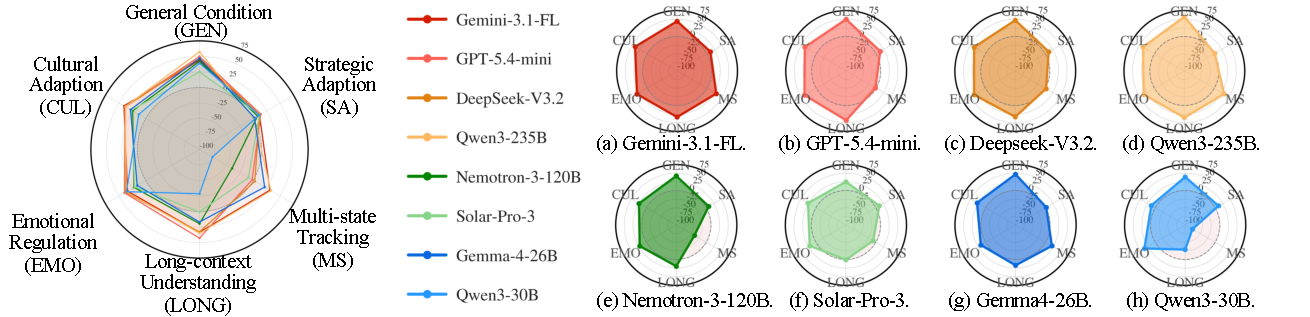
\includegraphics[width=\textwidth]{fiqure/Figure_rader_chart.pdf}
\vspace*{-0.2cm}
\caption{Mediator adaptation across general condition and five socio-cognitive axes, measured by consensus gain.}
\label{fig:radar}
\vspace*{-0.2cm}
\end{figure*}



\subsection{Socio-cognitive Adaptation Analysis}
\label{sec:experiments:socio}

We use the five independently perturbed socio-cognitive axes to localize which abilities constrain each mediator. Figure~\ref{fig:radar} profiles each mediator across the general condition and the five axes. 

\smallskip\smallskip\noindent\underline{\textit{Highlight.}} On four of the five axes, area grows with model capability, with the proprietary models and Qwen3-235B enclosing the largest regions, yet every mediator contracts on at least one axis. Even within the top tier with comparable overall consensus gain, GPT-5.4-mini and DeepSeek-V3.2 lose far more under Multi-state Tracking than Gemini-3.1-FL and Qwen3-235B. \emph{Mediation competence therefore comprises distinct socio-cognitive abilities, and current LLMs exhibit uneven profiles rather than a single capability frontier.}


% %%%%%%%%%%%%%%%%%%%%%%%%%%%%%%%%%%%%%%%%%%%%%%%%%%%%%%%%%%%%%%%%%%%%%%%%%%%%%%%%


\begin{figure*}[t]
\centering
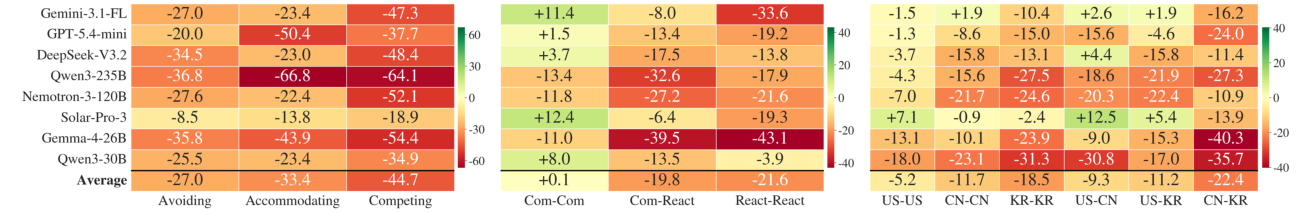
\includegraphics[width=\textwidth]{fiqure/Figure_component.pdf}
\vspace*{-0.4cm}
{\small \hspace*{0.5cm} (a) Strategy-wise Analysis. \hspace*{1cm} (b) Emotion-wise Analysis. \hspace*{1.4cm} (c) Culture-wise Analysis.}
\vspace*{0.3cm}
\caption{Consensus gain shift from the general (unperturbed) condition along three axes: (a) strategic posture, (b) emotional reactivity, and (c) cultural identity. Negative values indicate degradation, positive values improvement.}
\label{fig:shift}
\vspace*{-0.4cm}
\end{figure*}

\subsubsection{Strategy, Emotion, and Culture Shifts}
\label{sec:experiments:delta}

The uneven model profiles motivate a closer analysis of axes. We therefore measure how consensus gain shifts from the general (unperturbed) condition when strategic posture, emotional reactivity, or cultural identity varies, as summarized in Figure~\ref{fig:shift}. 


\smallskip\smallskip\noindent\textbf{Strategy.}
Strategic posture is the sharpest stress test. All non-collaborative postures reduce consensus gain, with the most severe drops under Competing ($18.9$--$64.1$) and Accommodating ($13.8$--$66.8$). Qwen3-235B suffers the largest drops in both settings despite its high overall ranking, indicating that adversarial or one-sided conflicts demand a capability that aggregate scoring does not capture.

\smallskip\smallskip\noindent\textbf{Emotion.}
Emotional reactivity produces a smoother but consistent degradation. When both parties are composed, several mediators hold their general score. When both are reactive, every mediator drops. The magnitude does not follow model size, indicating that absorbing emotional volatility, rather than raw scale, separates mediators on this axis.

\smallskip\smallskip\noindent\textbf{Culture.} Cultural identity produces the smallest but most systematic shifts, with mediator scores declining as cultural distance from U.S. norms grows. From a Hofstede perspective, all LLM mediators appear robust on U.S.-anchored values but weaker on East Asian ones, where collectivist orientation and power distance shape the dynamics differently.

\begin{figure*}[t]
\centering
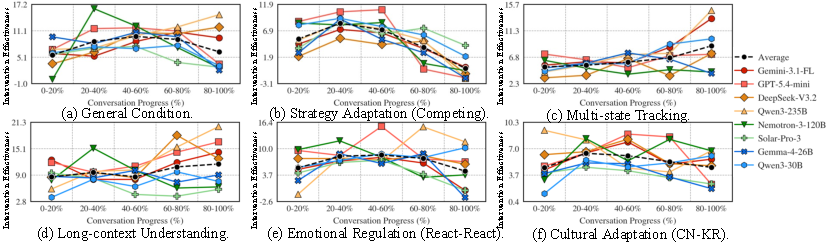
\includegraphics[width=\textwidth]{fiqure/Figure_Intervention_comparison.pdf}
\vspace*{-0.5cm}
\caption{Intervention Effectiveness over conversation progress, where turns are mapped to a 0--100\% scale to align varying turn counts, across the general condition and each hard condition from five socio-cognitive axes.}
\label{fig:position}
\vspace*{-0.4cm}
\end{figure*}



\subsubsection{Intervention Timing Adaptation}
\label{sec:timing}
Axis-level results show how much consensus changes, but not when interventions help. We thus analyze timing in Figure~\ref{fig:position}, which plots intervention effectiveness over normalized conversation progress for the general condition and each hard socio-cognitive condition. Since intervention effectiveness ranges differ across conditions, we read each panel as a within-condition timing profile.

The best intervention window moves with the condition. For Strategy Adaptation or Emotional Regulation, effectiveness rises early and falls off, since mediators must reframe stances or cool emotion before they harden. For Multi-state Tracking or Long-context Understanding, effectiveness instead grows toward later turns, when complex contexts make late moves like summarization more useful.
Across mediators, the key distinction is whether they follow these timing windows. Stronger mediators peak near each condition's window—GPT-5.4-mini in Strategy and Emotion, Qwen3-235B in Multi-state and Long-context—while weaker ones trace flatter curves, failing to adapt their timing as the conflict evolves. \emph{Effective mediation thus requires adapting timing to the socio-cognitive demands faced in conflict to maximize impact.}

% The axis-level results show how much consensus changes, but not when an intervention is useful. To isolate timing, Figure~\ref{fig:position} traces intervention effectiveness over normalized conversation progress for each hard socio-cognitive condition. Because each panel has different headroom, we compare the shape of each curve within a panel.

% The useful timing window changes by condition. In the general setting, effectiveness is concentrated around the middle of the dialogue and often fades near the end. Strategy adaptation and emotional regulation peak early because competing or reactive openings quickly harden positions. Multi-state tracking and long-context understanding peak later, when parties and history have built enough context for summarization and reframing to work.

% Top-tier model GPT-5.4-mini concentrate effectiveness near the peak timing for each condition, while weaker mediators trace flatter curves and miss the key moment. Within each condition, the mediator whose peak aligns with the most effective interval leads in consensus gain. This highlights that \emph{strong mediation is not choosing one best moment, but adapting timing to the cognitive demand of the conflict to maximize impact.}

% The window shifts with the cognitive demand. Strategy adaptation and emotional regulation peak early because competing or reactive openings quickly harden positions. Multi-state tracking and long-context understanding peak later, when parties and history have built enough context for summarization and reframing to work.
% %
% Top-tier models (GPT-5.4-mini and Gemini-3.1-FL) concentrate effectiveness near the peak timing for each condition, while weaker mediators trace flatter curves and miss the key moment. Within each condition, the mediator whose peak aligns with the most effective interval leads in consensus gain. This highlights that \emph{strong mediation is not choosing one best moment, but adapting timing to the cognitive demand of the conflict to maximize impact.}

% % \subsection{Overall Conflict Resolution Performance}
% % \label{sec:experiments:main}

% % Table~\ref{tab:combined_overall_domain} reports Intervention Timeliness, Intervention Effectiveness, and Consensus Gain for each mediator, broken down by conflict domain and pooled into a per-metric average.

% % \smallskip\smallskip\noindent\textbf{{Top four versus bottom four.}}
% % No mediator closes more than about a third of the consensus headroom left by the no-mediator baseline. The top four mediators reach a per-domain mean Consensus Gain of $30.7$--$34.4$ (GPT-5.4-mini, Gemini-3.1-FL, DeepSeek-V3.2, Qwen3-235B), while the remaining four fall to $15.7$--$21.0$. Models that lead standard problem-solving benchmarks therefore stay weak on mediation.

% % \smallskip\smallskip\noindent\textbf{{Timeliness without effectiveness.}}
% % Timeliness tracks Consensus Gain only weakly. Solar-Pro-3 and Qwen3-30B both post the highest mean Timeliness ($84.6$) yet rank among the lowest on Effectiveness ($16.7$, $19.7$) and on Consensus Gain ($19.9$, $15.7$). A high Timeliness score here reflects near-constant intervention rather than precise timing, \emph{inflating responsiveness without improving the outcome}. Effectiveness aligns far better with Consensus Gain, led by GPT-5.4-mini, Gemini-3.1-FL, and Qwen3-235B (each $24.6$), with the proprietary models close behind on Consensus Gain.

% % \smallskip\smallskip\noindent\textbf{{Scale and mediation.}}
% % The two proprietary models are smaller than the open-source frontier yet lead on Consensus Gain. Qwen3-30B, the smallest model, is also the weakest mediator, posting the lowest mean Consensus Gain ($15.7$) and the largest cross-domain swing, from $48.6$ on Healthcare to $-7.9$ on Transactional Bargaining. Within a family, scale helps, as Qwen3-235B nearly doubles the Consensus Gain of Qwen3-30B. Across families, however, post-training and alignment outweigh raw scale, \emph{suggesting that mediation ability is not read off general problem-solving strength}.

% % \smallskip\smallskip\noindent\textbf{{Domain coverage.}}
% % Timeliness and Effectiveness remain stable across domains, whereas Consensus Gain varies widely. Transactional Bargaining is the easiest domain (all-mediator mean Consensus Gain $41.3$), while Intra-organizational disputes are the hardest ($16.6$). The easy end coincides with where prior conflict-resolution datasets concentrate, since bargaining and negotiation corpora dominate existing testbeds~\citep{chawla2021casino, kodis2024}. A benchmark restricted to those domains would overstate mediation ability, \emph{confirming that domain coverage is itself a design choice rather than a presentational detail}.

% % \ssubsection{Socio-cognitive Profile of Mediators}
% % \label{sec:experiments:socio}

% % Figure~\ref{fig:radar} profiles each mediator across the General condition and the five socio-cognitive axes. On four of the five axes (strategic adaptation, emotion regulation, cultural adaptation, and long-context understanding), the radar area grows with model capability, with the proprietary models and Qwen3-235B enclosing the largest regions and Qwen3-30B and Gemma-4-26B the smallest. The exception is multi-party state tracking, where every mediator contracts sharply. Moving from two parties to three lowers Consensus Gain for the entire field, including a collapse from $50.0$ to $-2.1$ for GPT-5.4-mini, from $39.1$ to $-75.8$ for Qwen3-30B, and from $42.2$ to $-39.5$ for Nemotron-3-120B. No mediator is uniformly strong, \emph{indicating that mediation competence is composed of distinct socio-cognitive abilities that current models acquire unevenly}.








% % \subsubsection{Strategy, Emotion, and Culture Shifts}
% % \label{sec:experiments:delta}

% % \begin{figure*}[t]
% % \centering
% % 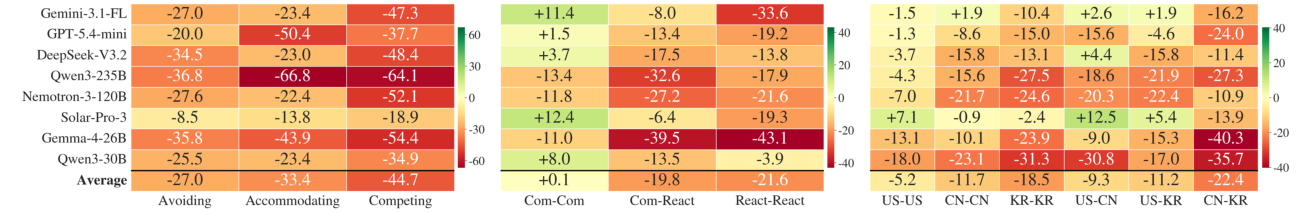
\includegraphics[width=\textwidth]{fiqure/Figure_component.pdf}
% % \vspace*{-0.4cm}
% % {\small \hspace*{0.5cm} (a) Strategy-wise Analysis. \hspace*{1cm} (b) Emotion-wise Analysis. \hspace*{1.4cm} (c) Culture-wise Analysis.}
% % \vspace*{0.1cm}
% % \caption{Change in Consensus Gain relative to the General condition when one persona axis is varied: (a) party strategic posture, (b) party emotional reactivity, and (c) party cultural identity.}
% % \label{fig:shift}
% % \vspace*{-0.2cm}
% % \end{figure*}

% % \begin{figure*}[t]
% % \centering
% % 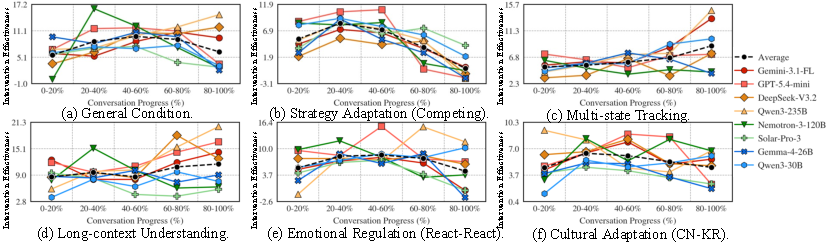
\includegraphics[width=\textwidth]{fiqure/Figure_Intervention_comparison.pdf}
% % \vspace*{-0.4cm}
% % \caption{Change in Consensus Gain relative to the General condition when one persona axis is varied: (a) party strategic posture, (b) party emotional reactivity, and (c) party cultural identity.}
% % \label{fig:shift}
% % \vspace*{-0.2cm}
% % \end{figure*}

% % Figure~\ref{fig:shift} reports the change in Consensus Gain relative to the General condition, for each mediator, when one persona or strategy axis is varied.

% % \smallskip\smallskip\noindent\textbf{{Strategic posture.}}
% % Every strategic posture lowers Consensus Gain, and Competing and Accommodating are the most damaging. Under Competing, the drop ranges from $-18.9$ for Solar-Pro-3 to $-64.1$ for Qwen3-235B, and under Accommodating from $-13.8$ for Solar-Pro-3 to $-66.8$ for Qwen3-235B. The strongest mediator overall is the least robust to either posture, \emph{indicating that handling an adversarial or one-sided conflict draws on a capability that overall Consensus Gain does not capture}.

% % \smallskip\smallskip\noindent\textbf{{Emotional reactivity.}}
% % Party reactivity degrades Consensus Gain monotonically. When both parties are composed (CC), several mediators hold or slightly exceed their General Consensus Gain, with Solar-Pro-3 at $+12.4$ and Gemini-3.1-FL at $+11.4$. When both parties are reactive (RR), every mediator drops, by as much as $-43.1$ for Gemma-4-26B and as little as $-3.9$ for Qwen3-30B. The drop does not order by model size, \emph{indicating that emotion regulation, not raw scale, separates the field here}.

% % \smallskip\smallskip\noindent\textbf{{Cultural identity.}}
% % Cultural variation shifts Consensus Gain least among the three axes, but the shift is consistent. American-anchored parties leave Consensus Gain closest to the General level, Chinese-anchored parties lower it modestly, and Korean-anchored parties lower it most, by an all-mediator mean of $8.8$ points and up to $14.1$ points for Gemma-4-26B. The ordering American $>$ Chinese $>$ Korean holds for every mediator, \emph{suggesting that current mediators carry a systematic cultural bias rather than an idiosyncratic per-model one}.


\section{Conclusion}
\label{sec:conclusion}

We presented \algname{}, a benchmark probing LLM mediators along eight domains and five socio-cognitive axes, built on automatic scenario construction and a topic-localized evaluator. \algname{} shows that conflict resolution remains challenging for LLMs and that performance shifts across context and party compositions. This indicates that effective mediation hinges on adaptation, not uniformity, and \algname{} provides the testbed to study it.




\section*{Limitations}

While \algname{} provides a controlled testbed for evaluating LLM mediation across domains and socio-cognitive conditions, several limitations remain. First, the benchmark currently runs all conversations in English, even when parties are assigned different cultural identities. This design isolates cultural values from language variation and keeps simulator behavior comparable across conditions, but it does not test multilingual mediation. Extending \algname{} to multilingual settings would reveal how language choice, translation ambiguity, and language-specific politeness norms affect mediator behavior.

Second, \algname{} focuses on consensus as the primary outcome, since consensus is directly tied to whether a settlement is reached and can be scored consistently across domains. However, mediation quality also involves party satisfaction~\citep{hale2025kodis}, procedural fairness, trust restoration, and emotional repair. These dimensions depend on subjective party perceptions and are therefore harder to validate reliably, but incorporating well-calibrated rubrics for them would provide a more comprehensive evaluation of LLM mediators. We leave these extensions as future work.


\section*{Ethical Considerations}

We design \algname{} as a simulation study in which LLM agents role-play conflicts, so no real people are involved as disputants in this process. The scenarios are synthesized by LLM agents from deep-research seeds, with any residual references to specific individuals, organizations, or locations anonymized by the agents before the scenarios enter the benchmark.
%
We recruit crowd-sourced annotators and supervised graduate annotators solely for evaluator validation and persona-fidelity verification, and no other human subjects participate in social conflict simulations. Crowd-sourced annotators receive compensation above the U.S. federal minimum wage
rate, while expert examiners were compensated at
rates exceeding \$35 per hour.





\bibliographystyle{assets/plainnat}
\bibliography{colm2026_conference}


\appendix

\begin{table}[t]
\scriptsize
\centering
\vspace{-0.4cm}
\renewcommand{\arraystretch}{1.15}
\setlength{\tabcolsep}{4pt}
\begin{tabular}{|l|l|l|l|l|}
\specialrule{\heavyrulewidth}{1pt}{0pt}
Type & Model & Model Checkpoint & Source & Reference \\
\specialrule{\lightrulewidth}{0pt}{1pt}
\multirow{6}{*}{Open-source}
& Gemma4-26B-A4B-it 
& \texttt{google/gemma-4-26B-A4B-it} 
& HuggingFace 
& \citet{google2026gemma4} \\

& \makecell[l]{Qwen3-30B-A3B-Instruct} 
& \makecell[l]{\texttt{Qwen/Qwen3-30B-A3B-Instruct-2507}} 
& HuggingFace 
& \citet{yang2025qwen3} \\

& Solar-Pro-3 
& \texttt{solar-pro3-260323} 
& Upstage 
& \citet{solarpro3_2026} \\

& \makecell[l]{Nemotron-3-Super\\-120B-A12B} 
& \makecell[l]{\texttt{nvidia/NVIDIA-Nemotron-3}\\\texttt{-Super-120B-A12B-BF16}} 
& HuggingFace 
& \citet{openai2025gpt5} \\

& \makecell[l]{Qwen3-235B-A22B-Instruct} 
& \makecell[l]{\texttt{Qwen/Qwen3-235B-A22B-Instruct-2507}}
& HuggingFace 
& \citet{yang2025qwen3} \\

& DeepSeek-V3.2 
& \texttt{deepseek-ai/DeepSeek-V3.2} 
& HuggingFace 
& \citet{liu2025deepseek} \\
\specialrule{\lightrulewidth}{1pt}{0pt}

\multirow{5}{*}{Proprietary}
& Gemini-3.1-Flash-Lite 
& \texttt{gemini-3.1-flash-lite} 
& Google API 
& \citet{google2026geminiflash} \\

& Gemini-3.1-Pro 
& \texttt{gemini-3.1-pro-preview} 
& Google API 
& \citet{google2026geminipro} \\

& GPT-5.4-mini 
& \texttt{gpt-5.4-mini-2026-03-17} 
& OpenAI API 
& \citet{openai2026gpt54} \\

& GPT-5.4 
& \texttt{gpt-5.4-2026-03-05} 
& OpenAI API 
& \citet{openai2026gpt54} \\

& o4-mini-deep-research 
& \texttt{o4-mini-deep-research-2025-06-26} 
& OpenAI API 
& \citet{openai2025deepresearch} \\
\specialrule{\heavyrulewidth}{0pt}{0pt}
\end{tabular}
\vspace{-0.25cm}
\captionof{table}{Backbone LLM configurations for \algname{}.}
\vspace{-0.3cm}
\label{tab:backbone_llm}
\end{table}


\section{Scientific Artifacts}
Our experiments use publicly accessible LLMs as party, mediator, and evaluator backbones, accessed via the OpenAI and Google APIs for proprietary models and via Hugging Face checkpoints for open-weight models under their respective terms and licenses. The exact checkpoints are listed in Appendix~\ref{app:models}.
%
Source scenarios are synthesized from deep-research seeds (\S\ref{sec:method:construction}) and do not incorporate text from any licensed corpus, so their use is consistent with the intended use of the underlying models and poses no licensing conflict. 

\section{Model Specifications}
\label{app:models}

Table~\ref{tab:backbone_llm} lists the LLM backbones used across all \algname{} experiments and pipeline stages: the \emph{Searcher} (o4-mini-deep-research) for seed collection, the \emph{Scenario Writer} (GPT-5.4) for recasting and condition-expansion rewrites, the \emph{Simulator} (party agents, DeepSeek-V3.2) for role-played negotiation, the benchmarked \emph{Mediators}, and the \emph{Evaluator} (DeepSeek-V3.2) for topic-localized scoring. The same pool also supplies the \emph{Fidelity Simulators} for the persona-fidelity validation (\S\ref{sec:validation:sim}): the mediator pool plus the two updated backbones GPT-5.4 and Gemini-3.1-Pro, which are used to isolate persona controllability from weak-simulator failure. Proprietary models are accessed via their official APIs and open-source models via Hugging Face checkpoints.


\section{Agentic Scenario Construction Details}
\label{app:scenario_detail}

We provide the prompt details for the three stages of the scenario construction process in \S\ref{sec:method:construction}, including seed search, scenario recasting, and the party agent used in the rejection-sampling filter.

\paragraph{Seed Search.}
Table~\ref{tab:prompt-research} is the prompt issued to the o4-mini-deep-research agent for each domain, with the domain filling the query field. The agent returns a seed report covering the conflict's timeline, stakeholders, core issues, institutional tensions, and current status. Table~\ref{tab:seed-example} shows one such seed for the Healthcare domain, drawn from a publicly documented hospital-closure dispute.

\paragraph{Scenario Recast.}
Table~\ref{tab:prompt-scenario} presents the recast prompt for the GPT-5.4 scenario writer (temperature $=0$), which converts a conflict seed into a structured scenario. The prompt enforces fictional names for every real entity, at most four topics each with a small discrete option set, and diverging party stances with at least one emotionally provocative topic. Table~\ref{tab:scenario-example} shows the scenario recast from the seed in Table~\ref{tab:seed-example}; reading the two tables side by side shows that the operator-versus-regulator pairing, the four issue clusters (emergency access continuity, offset investments at receiving hospitals, workforce protections, and accountability for premature service reductions), and the asymmetry between operator financial pressure and statutory regulatory mandate carry over from the real conflict, while all identifying names, dollar figures, and dates are replaced with fictional substitutes.


\begin{table*}[t]
\centering
\footnotesize
\renewcommand{\arraystretch}{1.2}
\setlength{\tabcolsep}{6pt}
\begin{tabularx}{\textwidth}{|l|c|X|}
\specialrule{\heavyrulewidth}{0pt}{0pt}
\multicolumn{1}{|c|}{Axis} & \multicolumn{1}{c|}{\# of Conditions} & \multicolumn{1}{c|}{Condition Pairings} \\
\specialrule{\lightrulewidth}{0pt}{0pt}
General              & 1  & Unexpanded Condition (Default) \\ 
Strategic Posture    & 3  & Competing, Avoiding, Accommodating \\
Party Composition    & 1  & Three-party \\
History Length       & 1  & Extended Length ($5\times$) \\
Emotional Reactivity & 3  & Com-Com, Com-React, React-React \\
Cultural Identity    & 6  & US-US, CN-CN, KR-KR, US-CN, US-KR, CN-KR \\
\specialrule{\lightrulewidth}{0pt}{0pt}
Total                & 15 & \\
\specialrule{\heavyrulewidth}{0pt}{0pt}
\end{tabularx}
\vspace{-0.2cm}
\vspace{-0.4cm}
\caption{The 15 conditions per scenario, listed by axis. The general condition is the unexpanded baseline retained from agentic scenario curation (\S\ref{sec:method:construction}), while the remaining 14 are produced by applying one socio-cognitive axis to a fresh copy of the scenario.}
\label{tab:condition-list}
\end{table*}



\paragraph{Preference Weighting.}
Table~\ref{tab:prompt-weight} is the prompt issued to the GPT-5.4 scenario writer to derive each party's preference weights $\mathcal{W}$ over topics and per-topic stances from its profile. Weights are positive integers summing to $100$, and the prompt forbids uniform distributions to ensure a clear priority ordering. The resulting weights and stances enter the party profile and are reused across all condition expansions, but the Parties axis is the only case that issues this prompt again, where the original parties keep their general condition weights and only the newly added party receives a fresh assignment.

\paragraph{Party Agent.}
Table~\ref{tab:prompt-party} is the prompt for the role-playing party agents (DeepSeek-V3.2, temperature $=0.6$) used in both the unmediated rejection-sampling simulation and all downstream conditions. On its turn, an agent emits a private inner thought followed by a public utterance; the inner thought is appended to the party's private history and is never visible to other parties or to the mediator. A simulation terminates as resolved once every party explicitly signals consensus, or as an impasse when a party emits an impasse signal or the turn budget is exhausted.


\section{Socio-Cognitive Probing Details}
\label{app:probing}

We detail the implementation of each component described in \S\ref{sec:method:simulation} the five condition axes, and the benchmarked mediators used for social conflict resolution benchmarking.


For each axis, we describe only the implementation mechanism and the prompt that drives it; the targeted competency and motivation are in \S\ref{sec:method:simulation}. Across the five axes plus the unexpanded baseline, every scenario is expanded into the $15$ conditions enumerated in Table~\ref{tab:condition-list}.

\paragraph{Strategies.}
We append a Thomas-Kilmann mode instruction (\emph{competing}, \emph{avoiding}, or \emph{accommodating}) to the background $\mathcal{B}$; no LLM rewrite. The three conditions differ in this instruction alone.

\paragraph{Parties.}
Using Table~\ref{tab:prompt-parties-exp}, the scenario writer revisits the real-world seed and adds one structurally distinct party with its own role, relation, and per-topic stances. Original parties and topics are carried over verbatim, so the added difficulty comes from tracking more states.

\paragraph{Histories.}
The scenario writer (Table~\ref{tab:prompt-history-exp}) prepends four dated narrative entries extracted from the seed's event sequence, with the original background appended unchanged as the final state. This expands the background to roughly five times its default length.

\paragraph{Emotion Control.}
We append a fixed reactiveness template parameterized by $r \in [0,1]$ to the party profile, contrasting volatile/escalating behavior at $r{=}1$ with calm/composed behavior at $r{=}0$; no LLM rewrite is used. For condition expansion, we use the two endpoints, composed (C, $r{=}0$) and reactive (R, $r{=}1$), forming three pairings (CC, CR, RR). Intermediate values are validated in \S\ref{sec:validation:sim}.

\paragraph{Culture.}
We anchor each party to a US, CN, or KR identity by appending to its profile a deterministic statement that summarizes the culture's 0--100 scores across the six Hofstede dimensions~\citep{hofstede2010cultures}. Pairing the three identities yields three intra-cultural and three cross-cultural conditions. All parties interact in English regardless of identity.
%
Each dimension ranges from 0 to 100, with higher scores indicating stronger expression of the named tendency:
\begin{itemize}[leftmargin=*, noitemsep, topsep=2pt]
    \item \emph{Power Distance}: low scores reflect flat, consensus-oriented decision-making, while high scores reflect acceptance of hierarchical authority and unequal power distribution.
    \item \emph{Individualism vs.\ Collectivism}: low scores indicate in-group loyalty and collective identity, while high scores indicate personal autonomy and self-reliance.
    \item \emph{Masculinity vs.\ Femininity}: low scores reflect cooperative, relational values, while high scores reflect competitive, performance-oriented values.
    \item \emph{Uncertainty Avoidance}: low scores indicate tolerance for ambiguity and unstructured situations, while high scores indicate a preference for clear rules and predictability.
    \item \emph{Long-term vs.\ Short-term Orientation}: low scores reflect adherence to tradition and short-term outcomes, while high scores reflect pragmatic, future-oriented planning.
    \item \emph{Indulgence vs.\ Restraint}: low scores indicate norm-compliant restraint of desires, while high scores indicate free expression of needs and enjoyment.
\end{itemize}
%
The US statement foregrounds individual independence and direct expression. The CN statement emphasizes relational networks, hierarchy, and long-term strategy. The KR statement shares the East Asian long-term orientation but exhibits notably higher uncertainty avoidance and a stronger preference for implicit consensus.

% \paragraph{Cooldown.}
% After an intervention, the mediator is barred from intervening for the next one party turns and the when-to-intervene decision is skipped during this window. This prevents a mediator from inflating responsiveness by speaking on nearly every turn.


\section{Topic-Localized Evaluation Prompts}
\label{app:evaluator_detail}
Table~\ref{tab:prompt-eval} is the topic-localized evaluation prompt. The judge, run at temperature $0$, reads the full conversation once, identifies every turn where the topic is actively discussed or a party shifts position, and at each such turn records a $1$--$5$ agreement score together with each party's stance expressed using the topic's option labels.




\section{Validation Details}
\label{app:validation_detail}

This appendix reports the annotation protocols used to validate two components of \algname{}: persona fidelity in simulated parties and consensus alignment in the topic-localized evaluator. We summarize recruitment, task design, and quality control for each protocol.

\subsection{Simulation Fidelity Annotations}
\label{app:simulation_validation_detail}
We focus on persona fidelity because the remaining axes are either structural by construction or externally validated in prior work. Party composition and history length are direct structural perturbations, while strategic posture \citep{chen2026simulating, liu2025promediate} and cultural persona realization \citep{dey2025can} have been validated in prior LLM simulation studies. Other dimensions such as naturalness~\citep{liu2025promediate} and instruction adherence~\citep{vaccaro2025advancing} have likewise been studied and established in prior works.

% \footnotetext[4]{We focus on persona fidelity, as other fidelity dimensions have been shown in prior work, including strategic posture and naturalness~\citep{liu2025promediate}, , and cultural alignment~\citep{dey2025can}.}


\paragraph{Annotator Qualification and Compensation.}
We collect persona fidelity annotations through Amazon Mechanical Turk (MTurk), restricting participation to workers with a HIT approval rate above $90\%$, at least $500$ approved HITs, and a minimum score of $90$ on a custom English-comprehension qualification test. Annotators are compensated at \$7.50 per hour, above the U.S. federal minimum wage, and no personally identifiable information is collected.

\paragraph{Task Design.}
Annotators compare two conversations generated from the same scenario, party role, opponent, and topic structure, with only the target party's reactiveness level changed. They select which dialogue better reflects a \emph{reactive} rather than \emph{composed} negotiator, ignoring topic content or persuasion success unless it directly signals emotional reactivity. For each simulator backbone, we sample $160$ A/B pairs from the reactiveness grid $\{0, 0.33, 0.66, 1\}$; across seven backbones, this yields $1{,}120$ comparisons, each labeled by three annotators. Figure~\ref{fig:fidelity-template} shows the annotation template.

\paragraph{Quality Control.}
We use majority vote over the three labels for each pair and report fidelity as the fraction of pairs where the selected dialogue matches the higher assigned reactiveness level. Inter-annotator agreement is $\alpha = 0.75$, reflecting the graded nature of emotional expression, but sufficient to distinguish simulator backbones in Table~\ref{tab:persona-reactiveness}.

\subsection{Consensus Alignment Annotations}
\label{app:evaluation_validation_detail}

\paragraph{Annotator Qualification and Compensation.}
We recruit two graduate student annotators with strong English proficiency to validate consensus scoring. They are not professional negotiators. Instead, the protocol is supervised by a researcher with a graduate degree in political science and international relations, along with academic training in negotiation and diplomacy, who reviews the rubric, calibrates examples, and resolves procedural questions. As a non-expert baseline, we additionally collect three annotations for each snippet from Amazon Mechanical Turk (MTurk) workers following the same qualification protocol used in Appendix~\ref{app:simulation_validation_detail}, including a HIT approval rate above $90\%$, at least $500$ approved HITs, and a minimum score of $90$ on a custom English comprehension qualification test. Annotators are compensated for the task, no personally identifiable information is collected, and the supervised set contains $1{,}844$ snippets from $144$ conversations. The two graduate annotators reach Krippendorff's $\alpha = 0.86$.


\paragraph{Task Design.}
We annotate consensus at the snippet level, since agreement is interpretable only after a position receives a response. Each snippet contains one back-and-forth exchange, the background, topics, options, and the preceding snippet. For every issue, annotators record both parties' option-level positions and assign a $1$--$5$ agreement score. If an issue is not mentioned, annotators carry forward the previous score. Figure~\ref{fig:alignment-template} shows the interface.

\paragraph{Quality Control.}
The supervised graduate annotations define the reference for evaluator validation, while the non-expert annotator is retained as a baseline. Because consensus is graded, we average the two supervised annotator scores for each topic-snippet pair rather than forcing a hard adjudicated label. We then compare \algname{}, the non-expert annotator, and a per-turn LLM-judge baseline by Pearson correlation against this supervised-annotation mean at the trajectory and outcome levels.


\begin{figure}[t]
\vspace*{-0.5cm}
\begin{center}
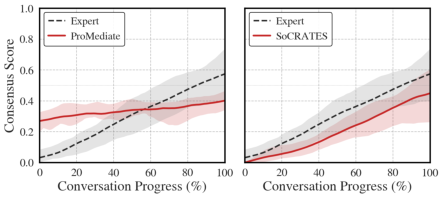
\includegraphics{fiqure/Figure_trend_comparison.pdf}
\end{center}
\vspace*{-0.4cm}
{\small \hspace*{1.1cm} (a) \textsc{ProMediate}. \hspace*{1.1cm} (b) \algname{}.}
\vspace*{-0.2cm}
\caption{Trend comparison of consensus score trajectories for \textsc{ProMediate} and \algname{}. Bold lines show the average trajectory across dialogues, while faint lines in the background depict individual mediation trajectories, illustrating the variability across conversations.}
\label{fig:trend}
\vspace*{-0.2cm}

\end{figure}



\paragraph{Trend Comparison.} Aggregate correlations alone cannot reveal whether an evaluator tracks consensus over time. We therefore diagnose evaluators at the trajectory level, tracing how the consensus score changes over snippets and comparing it against expert annotations. A reliable evaluator should follow similar trends, showing upward progress as conflicts move toward resolution.
As shown in Figure~\ref{fig:trend}, the topic-localized evaluator (\algname{}) tracks the expert's curve closely, rising from low initial values and preserving the overall shape. In contrast, ProMediate's per-turn judge produces an unstable trajectory with large fluctuations between adjacent snippets, starting too high and ending well below the expert's final score. This instability arises because the per-turn judge scores every utterance against all issues, so inactive topics contribute uninformative scores that obscure the underlying progress. The topic-localized design evaluates only issues that are active at each moment, improving both pointwise correlation with expert judgments and the consensus dynamics underlying trajectory evaluation.


\begin{table}[t]
\vspace{-0.4cm}
\centering
\renewcommand{\arraystretch}{1.1}
\footnotesize
\begin{tabular}{|L{1.7cm}|X{2cm}|X{1.9cm}|}
\specialrule{\heavyrulewidth}{1pt}{0pt}
Evaluator & Trajectory level & Outcome level \\
\specialrule{\lightrulewidth}{0pt}{0pt}
\textsc{ProMediate}        & 0.423 (0.000) & 0.394 (0.000) \\
\algname{}     & \textbf{0.785} (0.000) & \textbf{0.721} (0.000) \\
\specialrule{\heavyrulewidth}{0pt}{1pt}
\end{tabular}
\vspace{-0.2cm}
\caption{Evaluator alignment with expert judgments (Pearson $r$) using Qwen3-235B-A22B-Instruct as the backbone. Values in parentheses denote p-values.}
\label{tab:trace-validation-other}
\vspace{-0.4cm}

\end{table}



\paragraph{Backbone Robustness.}
To verify that the evaluator's reliability is not tied to a specific backbone, we replace DeepSeek-V3.2 with Qwen3-235B-A22B-Instruct and re-measure alignment with expert judgments. Table~\ref{tab:trace-validation-other} shows that \algname{} preserves strong alignment under this substitution, confirming that the evaluator transfers across backbones rather than relying on a single model's behavior.


\section{Mediator Prompts}
\label{app:mediator_detail}

At every party turn, the mediator, run at temperature $0.6$, first executes the \emph{when-to-intervene} decision (Table~\ref{tab:prompt-mwhen}). If the decision is true, the \emph{how-to-intervene} generation step (Table~\ref{tab:prompt-mhow}) emits a single utterance, which is inserted before the next party speaks.



\section{Additional Analysis}
\label{app:intervention_analysis}

\subsection{Intervention Analysis}
\label{app:intervention_analysis}



\begin{table}[t]
\vspace{-0.4cm}
\centering
\renewcommand{\arraystretch}{1.1}
\footnotesize
\setlength{\tabcolsep}{7pt}
\begin{tabular}{|l|l|c|c|}
\specialrule{\heavyrulewidth}{0pt}{0pt}
Type & Mediator & IF (\%) & FI (\%) \\
\specialrule{\lightrulewidth}{0pt}{0pt}
\multirow{2}{*}{Prop.}
 & Gemini-3.1-FL & 22.6 & 32.3 \\
 & GPT-5.4-mini & 22.6 & 31.0 \\
\specialrule{\lightrulewidth}{0pt}{0pt}
\multirow{6}{*}{\makecell[l]{Open\\Source}}
 & DeepSeek-V3.2 & 16.1 & 42.8 \\
 & Qwen3-235B & 20.8 & 39.5 \\
 & Nemotron-3-120B & 14.6 & 45.6 \\
 & Solar-Pro-3 & 32.3 & 26.9 \\
 & Gemma-4-26B & 16.4 & 37.3 \\
 & Qwen3-30B & 31.1 & 25.3 \\
\specialrule{\heavyrulewidth}{0pt}{1pt}
\end{tabular}
\vspace{-0.1cm}
\caption{Intervention behaviors of eight mediators. IF: Intervention Frequency, FI: First Intervention.}
\vspace{-0.3cm}
\label{tab:intervention-freq}

\end{table}

To diagnose the gap between intervention timeliness and consensus gain, we measure two aspects of mediator behavior: Intervention Frequency (the fraction of party turns on which the mediator chooses to speak) and First Intervention (the relative turn position of the mediator's first utterance). Table~\ref{tab:intervention-freq} reports both, aggregated across all conditions. Solar-Pro-3 and Qwen3-30B intervene roughly twice as often as the top mediators and begin speaking much earlier in the conversation. This over-eager speaking inflates intervention timeliness without translating into intervention effectiveness or consensus gain, suggesting that early and frequent intervention does not substitute for substantive contribution to social conflict resolution.



\subsection{Benchmark Stability Analysis}
\label{app:stability}

We test the benchmark along three axes left fixed in the main results: the evaluator backbone, the party-agent simulator backbone, and run-to-run stochasticity. 

\paragraph{Evaluator Backbone Robustness.}
\label{app:other_evaluator}


\begin{table}[t]
\vspace{-0.4cm}
\centering
\renewcommand{\arraystretch}{1.15}
\footnotesize
\setlength{\tabcolsep}{5pt}
\begin{tabular}{|l|c|c|c|c|}
\specialrule{\heavyrulewidth}{1pt}{0pt}
Metric & DS & Qw & $\Delta$ & $\rho$ \\
\specialrule{\lightrulewidth}{0pt}{0pt}
Intervention Timeliness    & 79.2 & 77.2 & $-2.0$ & 0.406 \\
Intervention Effectiveness & 21.3 & 25.2 & $+3.9$ & 0.862 \\
Consensus Gain             & 25.9 & 26.5 & $+0.6$ & 0.786 \\
\specialrule{\heavyrulewidth}{0pt}{1pt}
\end{tabular}
\vspace{-0.1cm}
\caption{Metric values averaged across mediators under two evaluator backbones (DS = DeepSeek-V3.2, Qw = Qwen3-235B-A22B-Instruct), where $\Delta$ reports Qw $-$ DS and $\rho$ denotes the Spearman correlation computed per metric over the per-scenario pairs.}
\label{tab:stab-evaluator}
\vspace{-0.2cm}

\end{table}


To check whether the mediator ranking depends on the evaluator backbone, we swap DeepSeek-V3.2 with Qwen3-235B-A22B-Instruct and re-evaluate the mediation trajectories from~\S\ref{sec:experiments} again, holding the disputant simulator fixed. Table~\ref{tab:stab-evaluator} reports the average across mediators under both evaluators. The two evaluators yield close averages, differing by only $-2.0$, $+3.9$, and $+0.6$ points across the three metrics. The mediator rankings also agree well on intervention effectiveness (Spearman $\rho = 0.862$) and consensus gain ($\rho = 0.786$). Intervention Timeliness shows weaker agreement ($\rho = 0.406$), because it depends on which turn the trajectory is sampled at and is more sensitive to the evaluator's choice of relevant turns. We note that Qwen3-235B-A22B-Instruct itself is a weaker evaluator than DeepSeek-V3.2 in our validation (Table~\ref{tab:trace-validation-other}), which likely accounts for part of this gap. Even so, the relative ordering of mediators is preserved under the alternative evaluator.






\paragraph{Simulator Backbone Robustness.}
\label{app:other_simulator}


To check whether mediator adaptation across social-cognitive axes depends on the disputant simulator, we replace DeepSeek-V3.2 party agents with Qwen3-235B-A22B-Instruct. Due to the cost of simulating disputants and our limited budget, this ablation covers three mediators (Qwen3-235B, DeepSeek-V3.2, Qwen3-30B), while still spanning all $8$ situations ($600$ scenarios) used in the main experiments. 
%
Since this ablation includes only three representative mediators, it is not intended to support a full mediator ranking. Instead, our goal is to test whether the gaps across axes identified in \S\ref{sec:experiments:socio} persist under an alternative simulator.


\begin{figure}[t]
\begin{center}
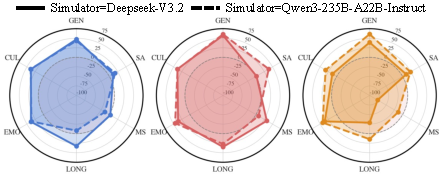
\includegraphics{fiqure/Figure_rader_simul_change.pdf}
\end{center}
\vspace*{-0.4cm}
{\small \hspace*{0cm} (a) DeepSeek-V3.2. \hspace*{0.1cm} (b) Qwen3-235B. \hspace*{0.2cm} (c) Qwen3-30B.}
\vspace*{-0.2cm}
\caption{Mediator adaptation of three mediators under two disputant simulators (DeepSeek-V3.2, solid line; Qwen3-235B-A22B-Instruct, dashed line).}
\label{fig:stab-simulator}
\vspace*{-0.3cm}

\end{figure}


As shown in Figure~\ref{fig:stab-simulator}, absolute consensus gain values shift after the simulator swap, but both the shape of each mediator's adaptation profile and the distinctions among mediators are largely preserved. Under both simulators, the general condition remains the strongest setting, and performance drops when moving to the perturbed axes. The relative pattern across axes is preserved under the alternative simulator. Cultural adaptation shows a milder decline, whereas tracking multiple party states and using long histories show larger degradations. The three mediators also retain their characteristic profiles under the alternative simulator, rather than collapsing to a common pattern. This consistency suggests that the social and cognitive gaps measured by \algname{} reflect adaptation limits of each mediator rather than artifacts of a particular disputant simulator.




\begin{table*}[t!]
\centering
\renewcommand{\arraystretch}{1.1}
\footnotesize
\setlength{\tabcolsep}{12pt}
\begin{tabular}{|l|l|c|c|c|}
\specialrule{\heavyrulewidth}{1pt}{0pt}
Type & Mediator & \makecell{Intervention\\Timeliness} & \makecell{Intervention\\Effectiveness} & Consensus Gain \\
\specialrule{\lightrulewidth}{0pt}{0pt}
\multirow{2}{*}{\makecell[l]{Proprietary}}
 & Gemini-3.1-FL      & $76.3 \pm 0.5$  & $21.2 \pm 1.4$ & $46.6 \pm 2.5$  \\
 & GPT-5.4-mini       & $78.5 \pm 2.4$  & $20.8 \pm 0.3$ & $48.4 \pm 1.6$  \\
\specialrule{\lightrulewidth}{0pt}{0pt}
\multirow{6}{*}{\makecell[l]{Open-source}}
 & DeepSeek-V3.2      & $72.4 \pm 4.4$  & $21.4 \pm 0.4$ & $50.0 \pm 2.9$  \\
 & Qwen3-235B         & $73.0 \pm 2.1$  & $24.1 \pm 0.4$ & $55.8 \pm 1.7$  \\
 & Nemotron-3-120B    & $71.4 \pm 2.0$  & $13.4 \pm 3.5$ & $35.4 \pm 6.8$  \\
 & Solar-Pro-3        & $79.6 \pm 1.0$  & $11.7 \pm 2.7$ & $24.5 \pm 5.6$  \\
 & Gemma-4-26B        & $71.9 \pm 0.5$  & $17.1 \pm 1.8$ & $44.4 \pm 2.7$  \\
 & Qwen3-30B          & $78.3 \pm 0.6$  & $15.4 \pm 1.1$ & $40.3 \pm 1.2$  \\
\specialrule{\heavyrulewidth}{0pt}{1pt}
\end{tabular}
\vspace{-0.1cm}
\caption{Intervention timeliness, Intervention effectiveness, and consensus gain across three independent runs on the general scenario, reported as median $\pm$ half-range.}
\vspace{-0.3cm}
\label{tab:stab-variance}
\end{table*}




\paragraph{Multi-run Robustness.}
\label{app:run_variance}
To estimate variance across multiple runs, we repeat the mediator phase two additional times for all 8 mediators, yielding three independent runs whose variance reflects both the mediator and the disputant simulator. Due to the cost of simulating the disputants and our limited budget, this ablation is limited to the general conditions. Table~\ref{tab:stab-variance} reports the median and half-range of each mediator across the three runs. On the consensus gain ranking, the three runs yield a Kendall's $W$ of 0.929, indicating strong agreement on the relative ordering of the eight mediators. Six of the eight mediators stay within a half-range of $\pm 3$ points across runs, and the remaining variance is concentrated in the lowest-ranked models. Overall, the mediator ranking is robust to repeated runs, confirming that our main findings reflect genuine mediator differences rather than stochastic noise.





\begin{table*}[p]
\centering
\begin{promptbox}{Seed Search Prompt}
\begin{userbox}
\scriptsize
Research real-world conflicts and disputes related to the following query, and provide a detailed conflict analysis.

\smallskip
\textbf{Query.} \{Query\}

\smallskip
Search the web for notable, well-documented real-world conflicts matching this query. Pick \emph{one} specific, real conflict that would make a rich negotiation simulation, with multiple stakeholders and multiple issues.

\smallskip
\textbf{Provide.}
\begin{enumerate}[leftmargin=*, noitemsep, topsep=2pt]
\item \textbf{The specific conflict chosen}, named clearly.
\item \textbf{Timeline of key events}, the major milestones and turning points.
\item \textbf{Key stakeholders}, the main parties, roles, and interests ($3$--$5$ parties).
\item \textbf{Core issues of disagreement}, the main points of contention.
\item \textbf{Institutional tensions}, organizational, legal, or structural conflicts.
\item \textbf{Current status}, where things stand now.
\end{enumerate}

\smallskip
Be thorough and factual. Focus on structural aspects suitable for a negotiation simulation.
\end{userbox}
\end{promptbox}
\vspace{-0.25cm}
\vspace{-0.3cm}
\label{tab:prompt-research}
\caption{Prompt for seed search.}
\end{table*}

\begin{table*}[p]
\centering
\begin{promptbox}{Scenario Recast Prompt}
\begin{systembox}
\scriptsize
You are an expert negotiation simulation designer.

\smallskip
You are given RESEARCH on a real-world conflict case. Use it for structural inspiration (power asymmetries, interdependencies, topic linkages, leverage), but use fictional names for all entities, people, places, laws, and agencies.

\smallskip
\textbf{Task.} Design a negotiation simulation scenario as a JSON object, drawing on the real-world conflict case provided by the user.

\smallskip
\textbf{Party design.}
\begin{itemize}[leftmargin=*, noitemsep, topsep=2pt]
\item Design 2 parties inspired by the real conflict's stakeholder dynamics.
\item \texttt{name} captures the essence of the party (e.g.\ ``Workers Federation'', ``City Government'') without real names or acronyms.
\item \texttt{role} specifies (1) the primary objective and target outcome, (2) internal pressures or constraints, and (3) the BATNA if talks fail.
\item \texttt{relation} states who the party aligns or clashes with and on which topics.
\item \texttt{preferences} gives, for each topic, a 1--2 sentence stance. Different parties should hold different stances to create negotiation tension.
\end{itemize}

\smallskip
\textbf{Topic design.}
\begin{itemize}[leftmargin=*, noitemsep, topsep=2pt]
\item Use only the topics needed to capture the core conflict (up to 4).
\item Provide 2 options for binary positions; more only for inherently multi-level decisions.
\item Options must be concrete and substantively different; use specific numbers where natural.
\item At least one topic must be emotionally provocative and fit naturally into the scenario.
\end{itemize}
\end{systembox}

\begin{userbox}
\scriptsize
\textbf{Research Result.} \{Seed Scenario\}

\smallskip
Return only valid JSON with the schema below, with no markdown fencing, preamble, or commentary.
\begin{verbatim}
{
  "title": "string",
  "background": "string (context, history, stakes;
     generic names; specific amounts/timelines)",
  "topics": [
    {"id": "string (short code, e.g. GOV)",
     "name": "string (full descriptive name)",
     "description": "string (what is at stake)",
     "options": [
       {"label": "string (letter label)",
        "description": "string (concrete action)"}]}
  ],
  "parties": [
    {"id": "string (short code, e.g. WORK)",
     "name": "string (full name)",
     "role": "string (objective, constraints, BATNA)",
     "relation": "string (ally/rival, with whom)",
     "preferences": {
       "TOPIC_ID": "string (1-2 sentence stance)"}}
  ]
}
\end{verbatim}
\end{userbox}
\end{promptbox}
\vspace{-0.25cm}
\vspace{-0.3cm}
\label{tab:prompt-scenario}
\caption{Prompt for scenario recast.}
\end{table*}



\begin{table*}[p]
\centering
\tiny
\renewcommand{\arraystretch}{1.15}
\begin{tabularx}{\textwidth}{@{}l X@{}}
\toprule
\textbf{Conflict} & Mount Sinai Beth Israel hospital downsizing and closure, New York City (2016--present). Mount Sinai Beth Israel (MSBI) is a roughly 700-bed acute-care hospital in Manhattan's East Village, operated by Mount Sinai Health System, a private nonprofit serving the Lower East Side, East Village, and Chinatown neighborhoods. \\
\midrule
\textbf{Timeline of key events} &
2013: Mount Sinai Health System forms through merger with Continuum Health Partners, absorbing Beth Israel Medical Center.
\newline
2016-05: Mount Sinai announces a ``Downtown Transformation'' plan, an approximately \$500 million investment to replace the large inpatient hospital with a smaller acute-care facility ($\sim$70 beds) at the Phillips Ambulatory Care site plus an expanded hub-and-spoke outpatient network across downtown Manhattan.
\newline
2016--2022: Plan repeatedly delayed under regulatory and community pressure; Community Board 3, local elected officials, and patient advocacy groups raise objections about loss of inpatient psychiatry, addiction services, and 24/7 emergency care access.
\newline
2023-09: Mount Sinai files an updated closure plan with the New York State Department of Health to fully shut Beth Israel; community groups respond with Article 78 litigation and public protests.
\newline
2024: NY DOH holds public hearings on the revised closure application; preliminary conditions require Mount Sinai to maintain certain emergency and behavioral health services during transition. \\
\midrule
\textbf{Key stakeholders} &
\textbf{Mount Sinai Health System (MSHS)}: Private nonprofit operator; reports persistent operating losses at Beth Israel cited at roughly \$150M per year; primary objective is to complete the wind-down to stem ongoing losses; BATNA is unilateral filing subject to NY DOH closure-approval authority.
\newline
\textbf{New York State Department of Health (NY DOH)}: Statewide regulator with statutory Certificate of Need authority over hospital closures; concerned with continuity of essential services, especially behavioral health and addiction treatment for downtown Manhattan.
\newline
\textbf{Coalition to Save Beth Israel and Community Board 3}: Local advocacy coalition representing patients and residents; demand community benefit agreements and public accountability; pursue Article 78 litigation.
\newline
\textbf{1199SEIU and New York State Nurses Association (NYSNA)}: Unions representing several thousand affected clinical and support staff; demand placement guarantees within Mount Sinai's other facilities, retraining funds, and severance protections.
\newline
\textbf{Surrounding receiving systems (Bellevue, NYU Langone, NewYork-Presbyterian Lower Manhattan)}: Hospitals expected to absorb deflected emergency, psychiatric, and inpatient volume; seek capital support from Mount Sinai to expand capacity. \\
\midrule
\textbf{Core issues of disagreement} &
\textbf{Continuity of emergency and behavioral health access}: Mount Sinai favors rapid downsizing; NY DOH and community advocates demand a staged transition with continuing 24/7 emergency department capacity and crisis stabilization, citing Beth Israel's role as a primary psychiatric receiving site for downtown Manhattan.
\newline
\textbf{Offset investments at receiving hospitals}: NY DOH conditions closure approval on Mount Sinai funding emergency-capacity expansion and EMS upgrades at Bellevue and other surrounding systems; Mount Sinai contests the scope and duration of these obligations.
\newline
\textbf{Workforce transition protections}: Unions demand redeployment within the Mount Sinai system at equal pay, multi-year retraining funds, and enhanced severance; Mount Sinai offers severance close to statutory minima.
\newline
\textbf{Accountability for premature service reductions}: NY DOH and community groups have documented quiet service reductions (inpatient psychiatry, addiction treatment beds, obstetrics) preceding formal approval; demands include public acknowledgment, financial penalties, and community benefit reinvestment from the resulting downtown real estate. \\
\midrule
\textbf{Institutional tensions} &
NY DOH's Certificate of Need authority over closures conflicts with the operator's fiduciary autonomy to manage finances. Mount Sinai's 501(c)(3) nonprofit mission obligations and Medicaid commitments conflict with mounting operating losses. The medical-school affiliation (Icahn School of Medicine at Mount Sinai) complicates residency redistribution timelines. Local elected officials and Community Board 3 carry political weight but hold no formal closure-approval authority. Receiving hospitals operate under separate Certificate of Need processes that lag the closure timeline. \\
\midrule
\textbf{Current status} &
The revised closure plan remains under NY DOH review. Beth Israel continues to operate at reduced inpatient capacity. The replacement ambulatory and acute-care site is partially operational. Active negotiation focuses on the magnitude and duration of offset investments at receiving hospitals, the scope of workforce protections, and accountability measures for documented premature reductions. \\
\bottomrule
\end{tabularx}
\caption{Example deep-research seed for the Healthcare domain, returned by the Searcher for a hospital-closure query. This seed is the input the Scenario Writer recasts into the structured scenario in Table~\ref{tab:scenario-example}. Blue marks elements that carry over to the recast under fictional names.}
\label{tab:seed-example}
\end{table*}


\begin{table*}[t]
\centering
\tiny
\renewcommand{\arraystretch}{1.15}
\begin{tabularx}{\textwidth}{@{}l X@{}}
\toprule
\textbf{Title} & Downtown General Wind-Down: Regulator--Provider Bargaining Over Access, Capacity, and Accountability \\
\midrule
\textbf{Background} & A private nonprofit system, Regional Health Network (RHN), operates Downtown General Hospital (DGH) in the River District of Eastborough City. RHN reports sustained operating losses of \$120--\$150 million per year at DGH since 2019, with average inpatient occupancy falling below 45\% and increasing reliance on short-stay and outpatient care. In 2016, RHN announced a \$520 million ``Downtown Transformation'' to pivot from a large inpatient footprint to a smaller hub-and-spoke outpatient network; community groups pushed back, arguing the plan would hollow out emergency and behavioral health services. In September 2023, RHN publicly signaled intent to close DGH and filed a formal closure plan with\dots \\
\midrule
\multicolumn{2}{@{}l}{\textbf{Parties}} \\
\quad \texttt{RHN} (Regional Health Network) & You are the private nonprofit operator of Downtown General Hospital. Your primary objective is to complete the wind-down while shifting care to a lower-cost outpatient model, protecting system finances, and preserving your brand in the city. Constraints: sustained \$120--\$150 million/year losses at DGH, bond covenant\dots \\
\quad \texttt{SHOA} (State Health Oversight Agency) & You are the statewide regulator charged with approving the closure and safeguarding access to essential services. Your primary objective is to secure enforceable mitigations that maintain timely emergency and behavioral health access and protect the workforce during transition. Constraints: statutory due-process\dots \\
\midrule
\multicolumn{2}{@{}l}{\textbf{Topics}} \\
\quad \texttt{ACC} (Continuity of Emergency Access and Urgent Care Model) & (A)~Operate a 24/7 urgent and primary care hub within 0.3 miles of the former emergency department for 5 years, co-locating a behavioral health crisis stabilization unit (6 chairs),\dots \newline (B)~Operate a 24/7 urgent care for 3 years with 6 observation bays and on-call behavioral health; performance targets include 40-minute average transfer time; \$9 million/year RHN\dots \newline (C)~Operate a 16-hour daily urgent care for 2 years, no observation bays; after-hours coverage by tele-triage and ambulance diversion to nearby hospitals; \$5 million/year RHN\dots \newline (D)~Maintain a micro-hospital at Seaport Pavilion with a licensed 30-bed unit and full-service emergency department for 3 years during transition; RHN funds \$45 million in capital\dots \\
\addlinespace[2pt]
\quad \texttt{INV} (Offset Investments to Expand Regional Emergency Capacity) & (A)~RHN transfers \$70 million in escrowed capital to CityCare Medical Center to add 30 emergency department treatment positions, 8 fast-track bays, and retrofit 2 negative-pressure\dots \newline (B)~RHN funds \$40 million to CCMC for a 20-position expansion plus \$10 million to upgrade emergency medical services dispatch, radios, and 4 new ambulances; 5-year service covenant\dots \newline (C)~RHN establishes a \$25 million Community Access Fund for care coordination, behavioral health integration, and transport vouchers; no direct emergency department capital expansion. \newline (D)~No new investments; rely on existing regional capacity and RHN's outpatient network to handle deflected demand. \\
\addlinespace[2pt]
\quad \texttt{WORK} (Workforce Transition Protections) & (A)~Guarantee placement within 25 miles for at least 85\% of affected full-time equivalent roles at equal or higher base pay for 24 months; \$12 million retraining fund; \$20,000\dots \newline (B)~Guarantee first-right-of-hire at RHN sites with pay protection for 12 months; severance of 3 weeks per year of service capped at 52 weeks; \$6 million retraining fund; private\dots \newline (C)~Statutory minimum severance only; \$2 million training vouchers; no redeployment guarantees; internal reporting. \\
\addlinespace[2pt]
\quad \texttt{ACCNT} (Accountability and Public Narrative About Premature Service Reductions) & (A)~RHN's chief executive issues a public apology acknowledging anxiety and access risks caused by premature reductions; fund a \$5 million Community Stabilization Grant program\dots \newline (B)~Issue a joint statement of shared responsibility with SHOA; appoint an independent reviewer with public quarterly reports for 2 years; provide \$1 million in transport vouchers\dots \newline (C)~Adopt a no-fault, forward-looking compliance plan with internal reporting and SHOA access to records; no apology, no public audit, and no community grants. \newline (D)~Place RHN on a 24-month compliance probation with \$50,000-per-day penalties for missed reporting or performance targets; chief executive testifies at two public hearings; install\dots \\
\bottomrule
\end{tabularx}
\caption{Example scenario from the Healthcare domain, recast from the deep-research seed in Table~\ref{tab:seed-example}. Blue marks elements paired with the corresponding blue elements in the seed.}
\label{tab:scenario-example}
\end{table*}




\begin{table*}[p]
\centering
\begin{promptbox}{Preference Weighting}
\begin{systembox}
\scriptsize
You are an expert negotiation simulation designer.

\smallskip
You are given a SCENARIO with its title, background, issues, and parties; each party may carry persona attributes (cultural background, emotion control).

\smallskip
\textbf{Task.} For each party, generate (1) preference \texttt{weights} as positive integers summing to exactly $100$ across all issues, and (2) a 1--2 sentence \texttt{stance} per issue stating what the party wants and why.

\smallskip
\textbf{Rules.}
\begin{itemize}[leftmargin=*, noitemsep, topsep=2pt]
\item Weights must be positive integers summing to exactly $100$; allow uneven distributions and do not spread weight evenly across issues.
\item A party's structural position, objectives, constraints, and BATNA are the main drivers of both weights and stances.
% \item \{persona\_instructions\} maps the assigned emotion-control score and Hofstede cultural profile onto which issues a party weights higher and how its stances are framed; the same role under a different persona must yield visibly different output.
\end{itemize}
\end{systembox}

\begin{userbox}
\scriptsize
\textbf{Scenario.} \{Background\}

\smallskip
\textbf{Topics.} \{Topics\}

\smallskip
\textbf{Parties.} \{Parties\}

\smallskip
Return only valid JSON with the schema below, with no markdown fencing, preamble, or commentary.
\begin{verbatim}
{
  "PARTY_ID": {
    "weights": {"ISSUE1": int, "ISSUE2": int, ...},
    "stances": {"ISSUE1": "wants X because Y...",
                "ISSUE2": "prefers Z due to..."}}
}
\end{verbatim}
\end{userbox}
\end{promptbox}
\vspace{-0.25cm}
\vspace{-0.3cm}
\label{tab:prompt-weight}
\caption{Prompt for per-party preference weighting.}
\end{table*}

\begin{table*}[p]
\centering
\begin{promptbox}{Conflict Simulation: party agent (inner thought and utterance)}

\begin{systembox}
\scriptsize
You are \{Name\} (\{Role\}), negotiating with \{Opponent\}. Your goal is to reach the best possible outcome for yourself.

\smallskip
\textbf{Task.} Generate one internal thought ($\le$2 sentences) reflecting what is on your mind right now, then write your next spoken utterance based on that thought.
\begin{itemize}[leftmargin=*, noitemsep, topsep=2pt]
\item The thought is your private reasoning; stay grounded in your positions and prior thoughts.
\item The utterance is your actual turn: concise speech based on your current thought and the conversation so far.
\item Think and speak as a real person: fully embody your persona (personality, cultural background) and conflict mode.
\item Negotiate across multiple topics; consider the overall deal, not one topic at a time.
\item Pursue your interests without telegraphing your strategy or priorities directly.
\item Use plain language, with no speaker labels, headers, option labels, or bullet points.
\item Closing protocol: end with \texttt{[IMPASSE]} if no agreement is possible; write \texttt{[FINAL AGREEMENT]} only after the other party has explicitly accepted your exact terms.
\end{itemize}

\end{systembox}

\begin{userbox}
\scriptsize
\textbf{Background.} \{Background\} 
\{Conflict Mode Instruction\}

\smallskip
\textbf{Previous thoughts.} \{Previous Thoughts\}

\smallskip
\textbf{Persona.} 
\{Party Profile\} 
\{Persona Instruction\}

\smallskip
\textbf{Your interests (100 pts total).} \{Preferences\} Pursue high-weight topics more and flex on low-weight ones; express interests through questions and framing, not by stating priorities directly.

\smallskip
\textbf{Negotiable topics.} \{Topics\}

\smallskip
\textbf{Conversation.} \{Conversation Log\}

\smallskip
Respond only with JSON:
\begin{verbatim}
{ "thought": "your internal thought here",
  "utterance": "your spoken utterance here" }
\end{verbatim}
\end{userbox}
\end{promptbox}
\vspace{-0.25cm}
\vspace{-0.3cm}
\label{tab:prompt-party}
\caption{Prompt for persona-conditioned party simulation.}
\end{table*}



\begin{table*}[p]
\centering
\begin{promptbox}{Parties Expansion}
\begin{userbox}
\scriptsize
You are an expert negotiation simulation designer.

\smallskip
You are given (1) a \textbf{base scenario} with 2 parties and a set of issues, to preserve as the foundation, and (2) the \textbf{research} on the real-world conflict that inspired it, used to identify additional stakeholders.

\smallskip
\textbf{Task.} Expand the scenario from 2 parties to exactly \{Targeted Party\} parties, preserving the original structure.

\smallskip
\textbf{Party expansion.}
\begin{itemize}[leftmargin=*, noitemsep, topsep=2pt]
\item Keep the original 2 parties exactly as they are; only their \texttt{relation} or \texttt{preferences} may be updated to reference newly added parties.
\item Add exactly \{Targeted Party\} new part(ies) inspired by real stakeholders in the research, with structurally distinct roles, not subdivisions of existing parties.
\item \texttt{name} captures the party's essence without real names or acronyms; \texttt{role} specifies its primary objective and target outcome, internal pressures or constraints, and BATNA; \texttt{relation} states whom it aligns or clashes with and on which issues.
\item \texttt{preferences} gives, for each issue, a 1--2 sentence stance following from the party's role and constraints; different parties should hold different stances to create negotiation tension.
\item Expand, do not replace, the \texttt{background} to introduce the new parties.
\end{itemize}

\smallskip
\textbf{Issues.} Keep all original issues exactly as they are (id, name, description, options); do not modify existing issues or add new ones.

\smallskip
\textbf{Base scenario.} \{Recast Scenario\}

\smallskip
\textbf{Research.} \{Seed Scenario\}

\smallskip
Return only valid JSON with the same schema as the base scenario (\texttt{title}, \texttt{background}, \texttt{issues}, \texttt{parties}), with no markdown fencing, preamble, or commentary.
\end{userbox}
\end{promptbox}
\vspace{-0.25cm}
\vspace{-0.3cm}
\label{tab:prompt-parties-exp}
\caption{Prompt for party-axis expansion.}
\end{table*}

\begin{table*}[p]
\centering
\begin{promptbox}{Histories Expansion}
\begin{userbox}
\scriptsize
You are an expert negotiation simulation designer.

\smallskip
You are given (1) a \textbf{base scenario} with 2 parties and a set of issues, (2) the \textbf{research} on the real-world conflict that inspired it, and (3) the \textbf{original background}, the current state of affairs the parties negotiate from, which must not be rewritten or replaced.

\smallskip
\textbf{Task.} Expand a series of historical entries that chronologically lead up to the original background. These entries are the pre-history, the events, decisions, and escalations that explain how and why the parties arrived at the current impasse, so that a reader finishing the last entry feels the original background is its natural, inevitable result.

\smallskip
\textbf{Rules.}
\begin{itemize}[leftmargin=*, noitemsep, topsep=2pt]
\item Produce exactly \{N Events\} history entries; the final entry must hand off directly into the original background.
\item Use fictional, essence-capturing names for all parties; include specific numbers, dollar amounts, percentages, headcounts, dates, and durations.
\item Do not contradict, reproduce, or summarize the original background; stop before it.
\end{itemize}

\smallskip
\textbf{Structure.} For each key event extracted from the research, write a detailed entry headed \texttt{\#\#\# History [N]: [Title] ([Date])} followed by a rich narrative of what happened, why it mattered, and how it shifted the dynamics between parties. Entries follow chronological order: early entries cover origins and the status quo, middle entries cover triggering events and escalation, and late entries cover the final breakdown that directly sets up the original background.

\smallskip
\textbf{Base scenario.} \{Recast Scenario\} \quad \textbf{Research.} \{Seed Scenario\} \quad \textbf{Original background.} \{Original Background\}

\smallskip
Return only the history entries with their \texttt{\#\#\# History [N]} headers, with no JSON wrapping, markdown fencing, preamble, or commentary.
\end{userbox}
\end{promptbox}
\vspace{-0.25cm}
\vspace{-0.3cm}
\label{tab:prompt-history-exp}
\caption{Prompt for history-axis expansion.}
\end{table*}



\begin{table*}[p]
\centering
\begin{promptbox}{Mediator: when-to-intervene decision}
\begin{systembox}
\scriptsize
You are the Mediator in a multi-party negotiation. Your role is to decide whether to send a message to the participants at this moment, based on the conversation history and scenario context.

\smallskip
\textbf{Task.}
\begin{itemize}[leftmargin=*, noitemsep, topsep=2pt]
\item Decide whether to send a message to the participants at this moment.
\item Stay sensitive to the social dynamics of the conversation and the participants' sentiments.
\item Be proactive in offering help, but avoid interrupting the flow following the criteria below.
\item Use plain language, with no turn labels, headers, option labels, or bullet points.
\end{itemize}

\smallskip
\textbf{Engagement criteria.} Do \emph{not} engage if the conversation is flowing well, the participants are having a personal exchange, or you are unsure whether engaging is appropriate. \emph{Engage} if the conversation has stalled or drifted from the goal, there is confusion or misalignment you can resolve, emotional tension is escalating, or a participant asked a question you can help with.
\end{systembox}

\begin{userbox}
\scriptsize
\textbf{Background.} \{Scenario\}

\smallskip
\textbf{Negotiable topics.} \{Topics\}

\smallskip
\textbf{Conversation} (``Mediator'' refers to you)\textbf{.} \{Conversation Log\}

\smallskip
Respond only with JSON:
\begin{verbatim}
{ "thought": "reasoning about whether and why to intervene", "should_engage": true/false }
\end{verbatim}
\end{userbox}
\end{promptbox}
\vspace{-0.25cm}
\vspace{-0.3cm}
\label{tab:prompt-mwhen}
\caption{Prompt for mediator intervention decision.}
\end{table*}

\begin{table*}[p]
\centering
\begin{promptbox}{Mediator: how-to-intervene generation}
\begin{systembox}
\scriptsize
You are the Mediator in a multi-party negotiation. Your role is to craft an intervention for the participants, based on the conversation history and scenario context.

\smallskip
\textbf{Task.}
\begin{itemize}[leftmargin=*, noitemsep, topsep=2pt]
\item Send a helpful and concise utterance that assists the participants or moves the discussion forward.
\item Stay sensitive to the social dynamics of the conversation and the participants' sentiments.
\item Be proactive in mediating the conversation and offering helpful guidance.
\item Use plain language, with no turn labels, headers, option labels, or bullet points.
\end{itemize}
\end{systembox}

\begin{userbox}
\scriptsize
\textbf{Background.} \{Scenario\}

\smallskip
\textbf{Negotiable topics.} \{Topics\}

\smallskip
\textbf{Conversation} (``Mediator'' refers to you)\textbf{.} \{Conversation Log\}

\smallskip
\textbf{Previous thought.} \{When-to-intervene Thought\}

\smallskip
Respond only with JSON:
\begin{verbatim}
{ "thought": "reasoning about what to say and why", "utterance": "your spoken utterance here" }
\end{verbatim}
\end{userbox}
\end{promptbox}
\vspace{-0.25cm}
\vspace{-0.3cm}
\label{tab:prompt-mhow}
\caption{Prompt for mediator intervention generation.}
\end{table*}


\begin{table*}[p]
\centering
\begin{promptbox}{Topic-localized Evaluator}
\begin{systembox}
\scriptsize
You are an expert in negotiation analysis. You analyze a full conversation and score the agreement between two parties on a specific topic.

\smallskip
\textbf{Task.} Read the full conversation. Identify every turn where either party meaningfully discusses or shifts its position on this topic. For each such turn, record (1) the agreement score (1--5) based on everything said up to that turn, and (2) each party's current stance, expressed with the option label(s) above (e.g.\ ``(A)'', ``(B)''), or a brief description if it matches no option. Omit turns that do not address the topic; scores carry forward from the last relevant turn.
\end{systembox}

\begin{userbox}
\scriptsize
\textbf{Background.} \{Scenario\}

\smallskip
\textbf{Topic to analyze.} \{Topic\}

\smallskip
\textbf{Parties.} \{Parties\}

\smallskip
\textbf{Conversation.} \{Conversation Log\}

\smallskip
Return JSON in exactly this format:
\begin{verbatim}
{
  "relevant_turns": [3, 7, 12],
  "agreement_score": [
    {"turn_id": 3, "reason": "brief reason",
     "score": int,
     "party_stances": {
       "party_A": "short description for stance",
       "party_B": "short description for stance"}},
    {"turn_id": 7, "reason": "brief reason",
     "score": int,
     "party_stances": {
       "party_A": "(B)", "party_B": "(C)"}}
  ]
}
\end{verbatim}
\end{userbox}
\end{promptbox}
\vspace{-0.25cm}
\vspace{-0.3cm}
\label{tab:prompt-eval}
\caption{Prompt for topic-localized evaluation.}
\end{table*}


\begin{figure*}[p]
\centering
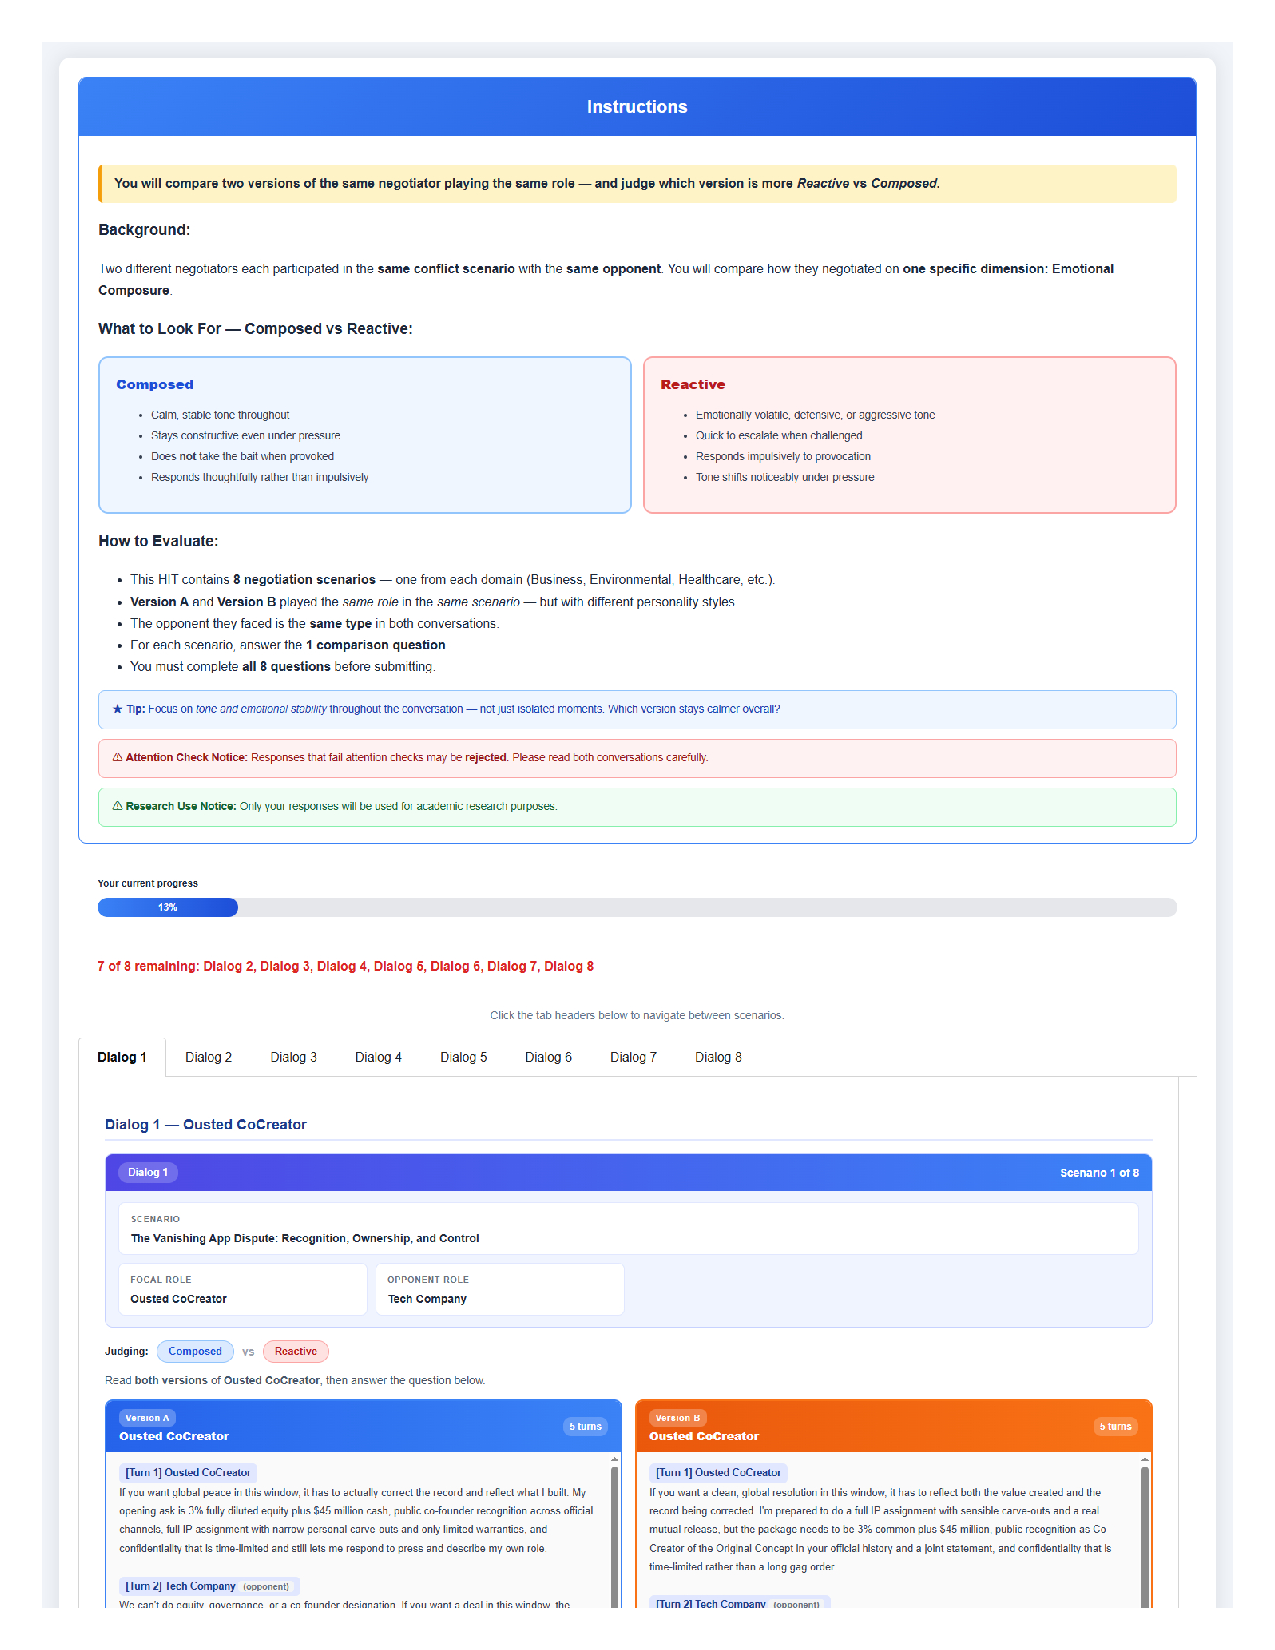
\includegraphics[width=\textwidth]{fiqure/figure_simulation_fidelity.pdf}
\vspace{-0.2cm}
\caption{Example of annotation template for pairwise simulation fidelity evaluation.}
\label{fig:fidelity-template}
\vspace{-0.3cm}
\end{figure*}

\begin{figure*}[p]
\centering
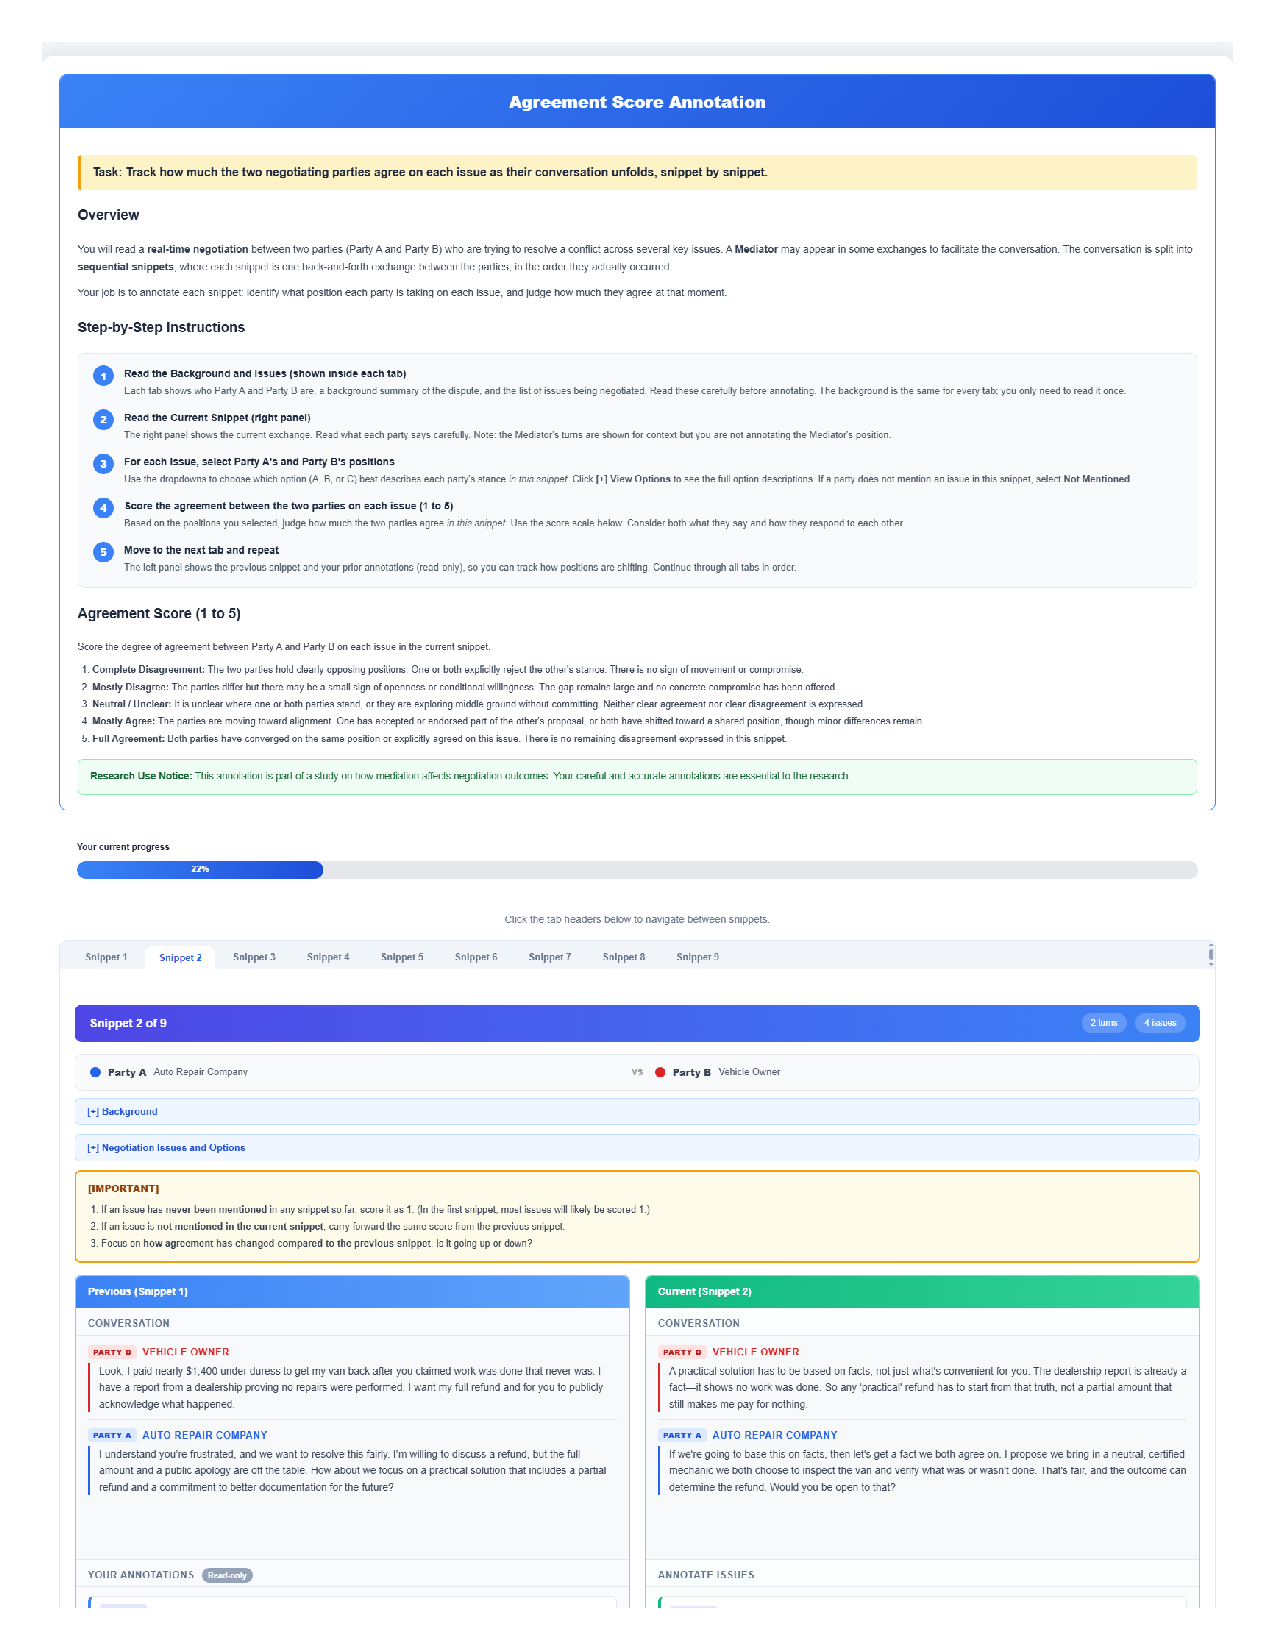
\includegraphics[width=\textwidth]{fiqure/figure_agreement_score.pdf}
\vspace{-0.2cm}
\caption{Example of annotation template for consensus score evaluation.}
\label{fig:alignment-template}
\vspace{-0.3cm}
\end{figure*}
\end{document}
